%% Template for Master thesis
%% ===========================
%%
%% You need at least KomaScript v3.0.0,
%% e.g. available in Texlive 2009
\documentclass  [
  paper    = a4,
  BCOR     = 10mm,
  twoside,
  fontsize = 12pt,
  toc      = bibnumbered,
  toc      = listofnumbered,
  numbers  = noendperiod,
  headings = normal,
  listof   = leveldown,
  version  = 3.03
]                                       {scrreprt}

% used pagages
\usepackage     [utf8]                  {inputenc}
\usepackage     [T1]                    {fontenc}
\usepackage                             {color}
\usepackage                             {amsmath, amssymb}
\usepackage                             {graphicx}
\usepackage     [english]               {babel}
\usepackage                             {natbib}
\usepackage                             {hyperref}

% my packages
\usepackage{bm}
\usepackage{subcaption}
\usepackage{multirow}
\usepackage{animate}           % for animated gifs
\usepackage{listings}          % for code

% my commands
\definecolor{lightgray}{gray}{0.9}
\newcommand{\inlinecode}[2]{\colorbox{lightgray}{\lstinline[language=#1]$#2$}}


% links
\definecolor{darkblue}{rgb}{0.0,0.0,0.4}
\definecolor{darkgreen}{rgb}{0.0,0.4,0.0}
\hypersetup{
    colorlinks,
    linkcolor=black,
    citecolor=darkgreen,
    urlcolor=darkblue
}

\begin{document}
  %% title pages similar to providet template instead of maketitle
  %% Titelseiten ähnlich zum Layout des Formulars von der
%% Fakultät für Physik und Astronomie
%%
%% Weitere Infos:
%% http://www.physik.uni-heidelberg.de/aktuelles/studium/
%% (PDF link: ...studium/download/145/Vorlage_Diplomarbeit_Formular.pdf)

%% Titelintro
\thispagestyle{empty}
\begin{center}
  \renewcommand{\baselinestretch}{2.00}
  \Large\sffamily
  Fakult\"{a}t f\"{u}r Physik und Astronomie\\
  \large
  Ruprecht-Karls-Universit\"{a}t Heidelberg
  \par\vfill\normalfont
  Masterarbeit\\
  Im Studiengang Physik\\
  vorgelegt von\\
  Martin Huber\\
  geboren in Frankenthal (Pfalz)\\
  2019\\
\end{center}
\newpage

%% Titelseite
\thispagestyle{empty}
\begin{center}
  \renewcommand{\baselinestretch}{2.00}
  \Large\bfseries\sffamily
    Implementierung und Fusion von \\
    modellprädiktiver Regelung mit \\
    neuronalen Netzwerken zur \\ 
    autonomen Navigation von humanoiden Robotern
  \par
  \vfill
  \large\normalfont
  Die Masterarbeit wurde von Martin Huber\\
  ausgeführt am\\
  Institut für Optimierung, Robotik und Biomechanik\\
  unter der Betreuung von\\
  Frau Prof. Katja Mombaur
  %% Bei externen Masterarbeiten hier noch den zweiten Betreuer einfügen
  %% und den vspace in Z. 45 entsprechend reduzieren
\end{center}\par
\vspace{5\baselineskip}

% Zeilenabstand zurücksetzen
\renewcommand{\baselinestretch}{1.00}\normalsize % select either german
  %% this will generate title pages similar to the template provided
%% by the Department of Physics and Astronomy Heidelberg
%%
%% More information:
%% http://www.physik.uni-heidelberg.de/aktuelles/studium/
%% (PDF link: ...studium/download/145/Vorlage_Diplomarbeit_Formular.pdf)

%% Titleintro
\thispagestyle{empty}
\begin{center}
  \renewcommand{\baselinestretch}{2.00}
  \Large\sffamily
  Department of Physics and Astronomy\\
  \large University of Heidelberg
  \par\vfill\normalfont
  Master thesis\\
  in Physics\\
  submitted by\\
  (name and surname)\\
  born in (place of birth)\\
  (year of submission)
\end{center}
\newpage

%% Titlepage
\thispagestyle{empty}
\begin{center}
  \renewcommand{\baselinestretch}{2.00}
  \Large\bfseries\sffamily
    (Title)\\
    (of)\\
    (Master thesis)
  \par
  \vfill
  \large\normalfont
  This Master thesis has been carried out by (Name Surname)\\
  at the\\
  (institute)\\
  under the supervision of\\
  (Frau/Herrn Prof./Priv.-Doz. Name Surname)
  %% additionally insert second supervisor here if carrying out an
  %% external diploma thesis. Reduce vspace in L. 44 accordingly.
\end{center}\par
\vspace{5\baselineskip}

% reset baselinestretch
\renewcommand{\baselinestretch}{1.00}\normalsize % or english title page
  %% Abstract page
%% =============
%%
%% Content of abstract pages has been put into seperate pages to simplify
%% word counting. Use e.g. the unix command
%%   wc abstract-ger.tex
%% or
%%   wc abstract-eng.tex
%% to get the number of words contained in these files.
\thispagestyle{empty}
\begin{center}
  \begin{minipage}[c][0.48\textheight][b]{0.9\textwidth}
    \small
    \textbf{
      Verhaltensklonung zur autonomen Navigation humanoider Roboter mit Nichlinearer Modellprädiktiver Regelung:
    }\par
    \vspace{\baselineskip}
    In dieser Arbeit erkunden wir die Möglichkeiten der Verhaltensklonung zur autonomen Navigation humanoider Roboter durch bloße Bilder. Hierfür wird eine nichtlineare, Modellprädiktive Regelung, die es ermöglicht, stabile Lauftrajektorien in Echtzeit zu erzeugen, implementiert und evaluiert. Es wird demonstriert, dass minimale Veränderung in der Bildverarbeitung genügen, um vielseitige Bewegungsstrategien in vielfältigen dynamischen und statischen Umgebungen zu erlernen. Diese Einfachheit der Lösung wird als passende Ergänzung zur Meidung von Konvexen Hindernissen identifiziert, welche durch Randbedingungen die Lösungen der nichtlinearen Modellprädiktiven Regelung einschränken. Alle Experimente werden an Heicub, einer Variente des iCub, durchgeführt, welcher speziell für Optimalsteuerung in der Fortbewegung am Istituto Italiano di Tecnologiia in Genove entwickelt wurde. Die Auswertung von Stabilitätskriterien zeigt weiterhin, dass ein menschlicher Kontrolleur, einem künstlichen Agenten gegenüber, nicht überlegen ist. Um die präsentierte Methode schließlich auf tauschende Aufgaben zu erweitern, vereinfachen wir die wechselnden Umgebungen auf ein gut gelöstes Klassifizierungsproblem.
  \end{minipage}\par
  \vfill
  \begin{minipage}[c][0.48\textheight][b]{0.9\textwidth}
    \small
    \textbf{
      Behavioral Cloning for Autonomous Navigation of Humanoid Robots with Nonlinear Model Predictive Control:
    }\par
    \vspace{\baselineskip}
    In this work, we investigate the capabilities of behavioral cloning for autonomous navigation of humanoid robots from raw image input. Therefore, a nonlinear model predictive control that allows for real-time generation of stable walking trajectories is implemented and evaluated. It is demonstrated that minor modifications in the vision pipeline are sufficient for the learning of versatile motion strategies in various dynamic and static environments. This simplicity is identified as a well-suited addition to the avoidance of convex obstacles, which are represented by constraints to the solution of the implemented nonlinear model predictive control. All of the experiments are carried out on Heicub, a descendant of the iCub, which was specially designed for optimal control in locomotion at the Istituto Italiano di Tecnologia in Genova. The evaluation of balance criteria further reveals that there is no superiority of a human controller over an artificial agent. Finally, we investigate on reinforcement learning methods to replace the behavioral cloning by self-taught policies.

  \end{minipage}
\end{center}


  \tableofcontents
  
  %% chapters
  \chapter{Introduction}
  % humanoids (icub, others), problem statement, research aim and objectives
    
  \chapter{State of the Art}
  \label{sec::2_sota}
  % contributions
    
  \chapter{Background}
  To generate dynamically balanced walking trajectories for humanoid robots and to let them navigate the environment autonomously, there are several posed challenges that we need to cover. As the logical starting point, in section \ref{sec::31_hm} - Humanoid Walking, we want to address the real time generation of walking trajectories for humanoid robots first, and then think of ways to replace the human user by an artificial agent in the control loop. As discussed in section \ref{sec::2_sota} - State of The Art, there are several ways to achieve this, but of particular interest to us are novel methods that evolved from the toolbox of machine learning techniques. Center to these new methods will be neural nets that we will try to train on solving the task of autonomous navigation in different ways, as shown in section \ref{sec::32_ml} - Machine Learning.
\begin{figure}[h]
	\centering
	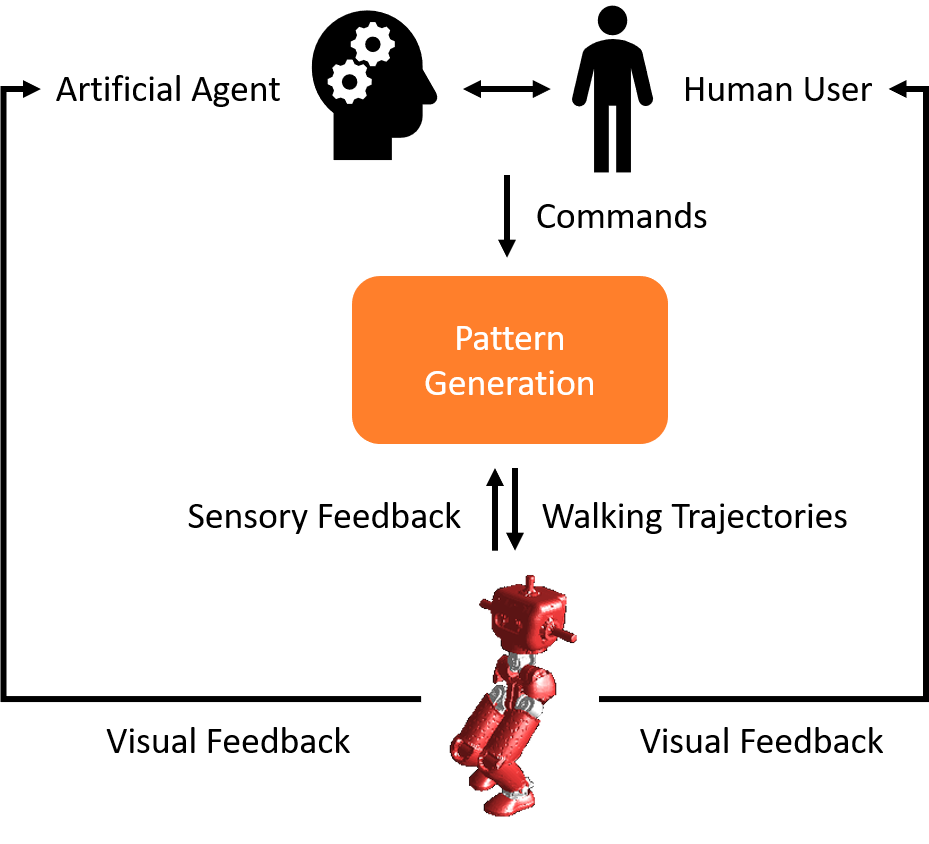
\includegraphics[scale=.5]{chapters/03_background/img/control_loop.png}
	\caption{\label{fig::3_cl} Proposed control loop to navigate the robot with either a human user or an artificial agent.}
\end{figure}   % introduction to background
  \section{Humanoid Walking}
\label{sec::31_hw}
To get started with and to understand the presented concepts that generate dynamically balanced walking trajectories, we shall have a look at figure \ref{fig::3_cl} once more. The pattern generation therein (orange box), consists of four main building blocks: Forward kinematics, nonlinear model predictive control (NMPC), interpolation, and inverse kinematics. The relation between these four building blocks is shown in fig. \ref{fig::31_pg}.
\begin{figure}[h]
	\centering
	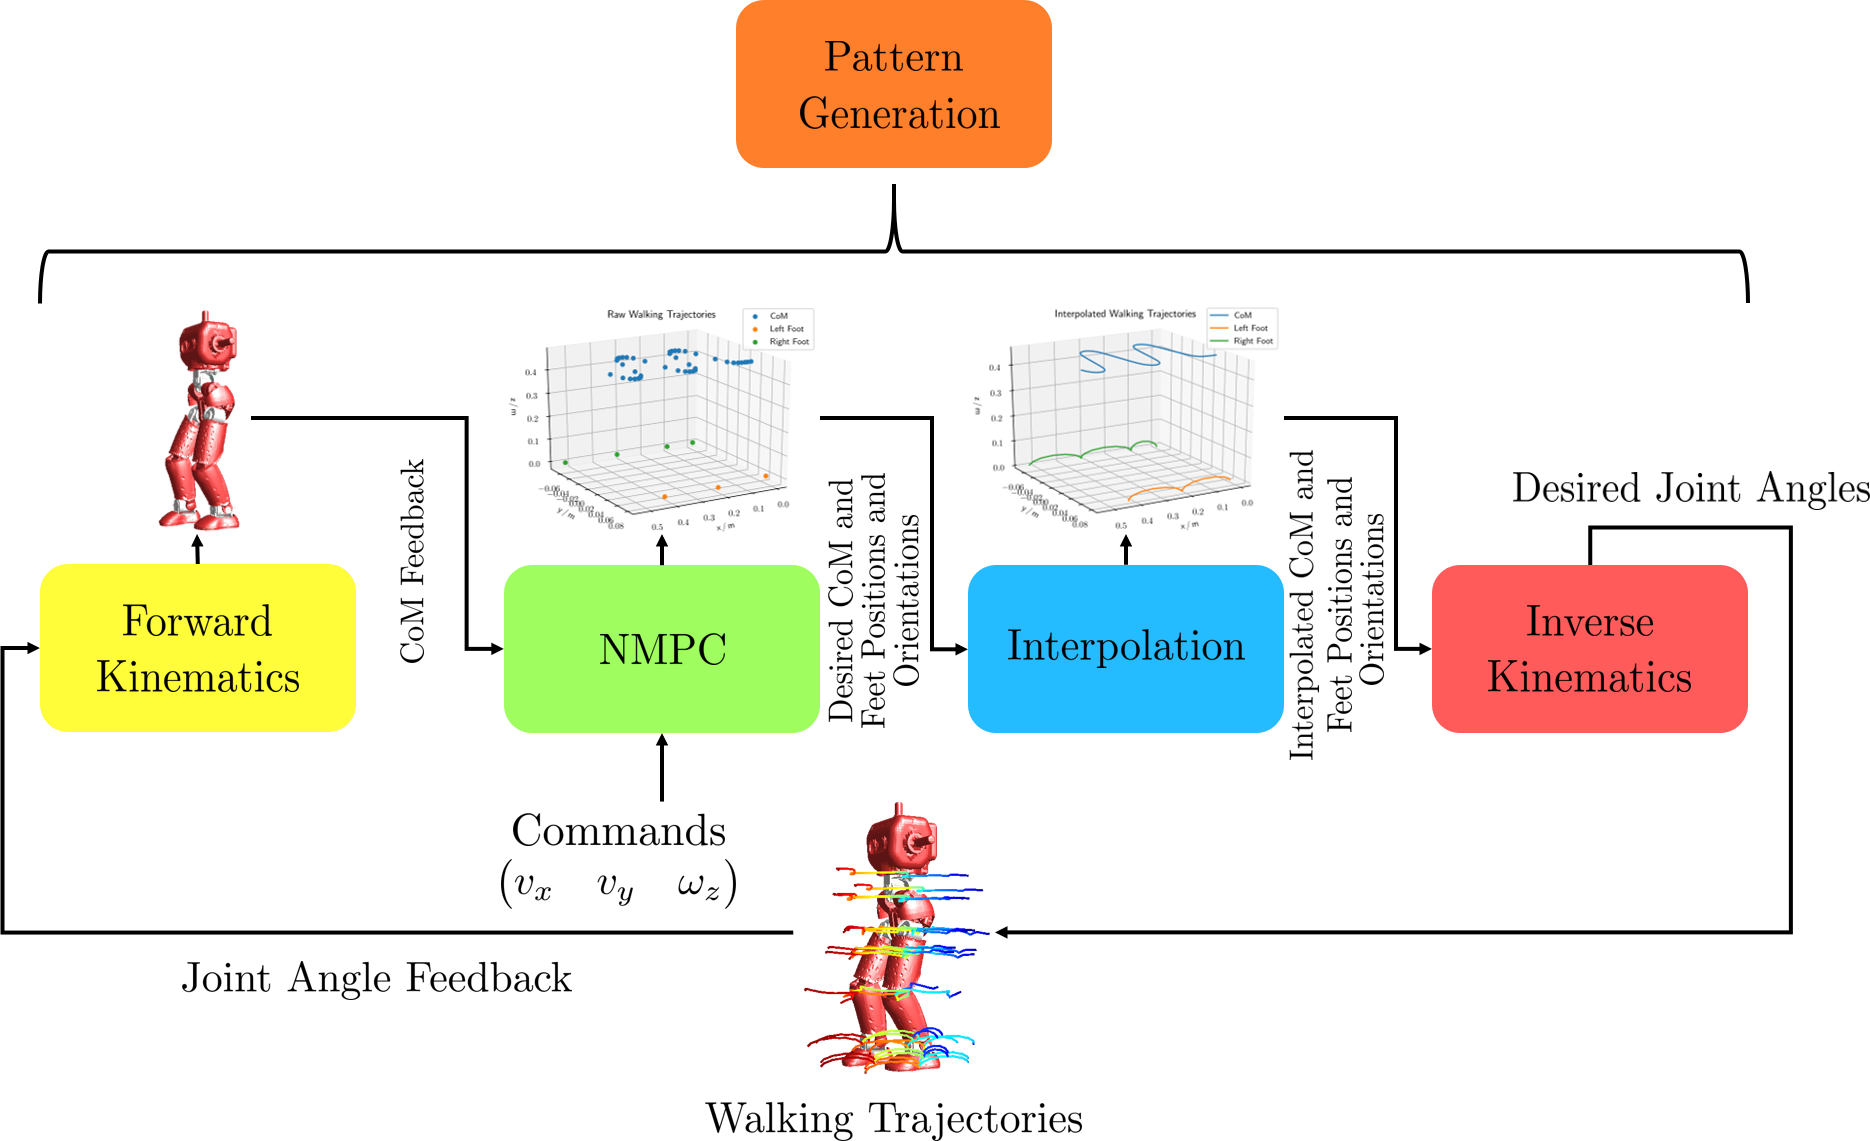
\includegraphics[scale=.5]{chapters/03_background/img/pattern_generation.png}
	\caption{Building blocks of the pattern generation. To understand the greater picture, a connection can be drawn to fig. \ref{fig::3_cl}, where the orange box represents the one shown in this figure.}
	\label{fig::31_pg}
\end{figure}
The natural entry point, to this otherwise closed control loop, is given by the commands that enter the nonlinear model predictive control. Commands are passed in the form of a desired velocity $\mathbf{v}_\text{ref}$ that the robot's center of mass (CoM) shall satisfy optimally according to a cost function that also takes dynamic balance and a smooth motion into account. The future desired positions and orientations for the CoM and the feet then result from the solution to a sequentially quadratic problem that tries to minimize this cost function. The balance criteria within this problem formulation is based upon the zero moment point (ZMP) around which the whole control framework is built. It is only by simplifying the robot's model that we can solve the optimal control problem in real time. Therefore, we assume the robot to be a linear inverted pendulum, for which we have a well defined analytical relation between the CoM and the ZMP. The minimization of the distance between the analytical expression of the ZMP and the foot placement results in the desired dynamic balance. As shown in fig. \ref{fig::31_pg}, the desired CoM and the feet positions and orientation, as they are obtained from the NMPC, are sparsely distributed in space. Moreover, there is neither information about how the feet shall move along the z-axis, nor along the x-, and y-axis, but only where they should be placed in the x-y-plane. Therefore, as the subsequent step to the NMPC, we need to add an interpolation. The interpolation interpolates the trajectories of the CoM to obtain a finer sampling time. Additionally, the movement of the feet in the x-, y-, and z-direction, as well as their orientation, is computed by polynomials that we require to satisfy the initial and end conditions of the foot placement. Put together, the nonlinear model predictive control and the interpolation between the resulting subsequent solutions for the positions and orientation of both, the CoM and the feet, describe dynamically balanced trajectories, given that the humanoid robot of interest resembles the physics of an inverted pendulum. Now to bridge the gap between dynamically balanced trajectories in Cartesian space, and a humanoid robot that actually satisfies them with its CoM and its feet, the inverse kinematics problem needs to be addressed. The inverse kinematics, which follow immediately after the interpolation step, take the positions and orientations of the CoM and the feet as constraints and find a composite of joint angles that fulfill them. The continuity of subsequent solutions is therein assured by initializing the inverse kinematics with the previous solution. Resulting joint angles, once passed to the humanoid, then result in walking trajectories, as indicated in fig. \ref{fig::31_pg} by the colored lines at the joints of the robot. Due to the inherent mismatch of the robot's physics from that of an inverted pendulum, as well as other effect like friction, there is a chance that the desired joint angles differ from the actually achieved ones. To compensate for the discrepancy, the last building block of the pattern generation is the feedback of the measured CoM to the NMPC. The CoM is computed by reading out the achieved joint angles, so that the forward kinematics can be utilized to determine the positions and orientations of the humanoid's links in space, and therefore the CoM.
\\\\
As already highlighted in the previous paragraph, special attention has to be given to the zero moment point, since it defines the central concept of the presented pattern generation. We therefore will explain its theoretical foundations, as well as its analytical relationship to the CoM for simplified physical models, and ways to measure it with force torque sensors in the section that lies ahead - Zero Moment Point.





    % short overview of humanoid walking
  \subsection{Zero Moment Point}
\label{sec::311_zmp}
The key metric in this work, for the generation of a dynamically balanced gait, is the zero moment point. The concept was first introduced by Miomir Vukobratovi\'{c} and Davor Juri\v{c}i\'{c} in 1968 \cite{vukobratovic1968contribution}\cite{vukobratovic1969contribution} and first utilized 1984 to generate walking trajectories for the WL-10RD robot \cite{yamaguchi1993development}. The most intuitive understanding for the ZMP arises by thinking about the realization of the simplest arbitrary possible walking motion for which a humanoid robot will not fall. This motion is achieved by ensuring the feet's whole area, and not only the edge, is in contact with the ground \cite{vukobratovic2004zero}, or put in other words, we require the robot not to rotate about its feet edges. This constraint can be met by having a reaction force $\bm{F}_r$ between the foot and the ground, which compensates for all external moments $\bm{M}_x$, and $\bm{M}_y$ around the x-, and y-axis at any time (fig. \ref{fig::311_zmp}).
\begin{figure}[h]
	\centering
	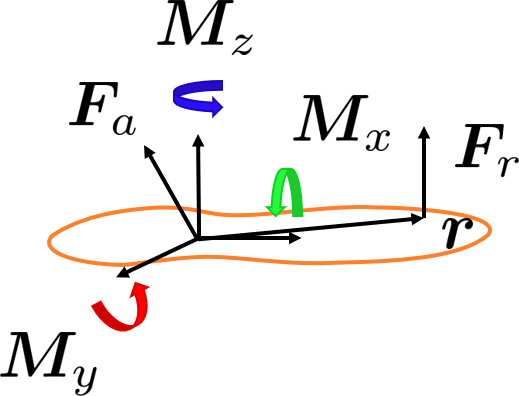
\includegraphics[scale=.5]{chapters/03_background/img/zero_moment_point.png}
	\caption{Forces acting on the sole.}
	\label{fig::311_zmp}
\end{figure}
The point $\bm{r}$, at which the reaction force acts, is physically only meaningful if it lies within the support polygon of the foot. Not only can it not exist outside of the support polygon, since there was no point of interaction between the foot and the ground then, but also was the robot to overturn under these circumstances. Therefore, the ZMP is defined as that point on the ground at which the net moment of the inertial forces has no component along the horizontal axes \cite{hirai1998development}\cite{dasgupta1999making}. We now came to appreciate the importance of the support polygon for the definition of the zero moment point. 
\begin{figure}[h]
	\centering
	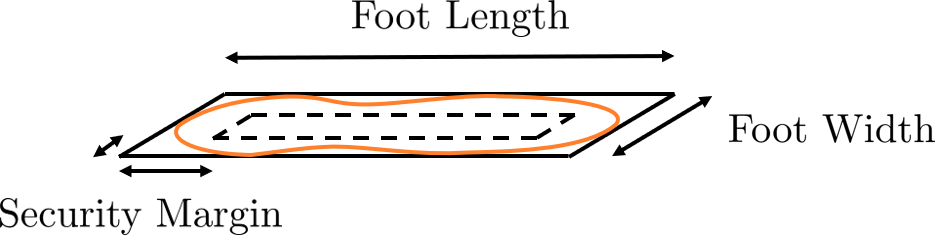
\includegraphics[scale=.5]{chapters/03_background/img/support_polygon.png}
	\caption{Full support polygon, and the resulting support polygon with security margin (dashed lines).}
	\label{fig::311_support_polygon}
\end{figure}
The support polygon is defined as the convex hull of all contact points of the feet with the ground, so the minimal number of points to fully contain all of them. As the most restrictive case for balance, in this work we will only consider the support polygon of one foot at a time. Since the convex hull of a foot is well described by a rectangle, we only rely on the foot width (\href{https://github.com/mhubii/nmpc_pattern_generator/blob/bc79a6d4f9bcfd3794146355af44429f5b7a9fe0/libs/pattern_generator/configs.yaml#L14}{link}), and foot length (\href{https://github.com/mhubii/nmpc_pattern_generator/blob/bc79a6d4f9bcfd3794146355af44429f5b7a9fe0/libs/pattern_generator/configs.yaml#L15}{link}) to fully describe it. Also, to ensure that the zero moment point never comes close to the edges of the feet and therefore to provide balance, we define a security margin to their boarders (\href{https://github.com/mhubii/nmpc_pattern_generator/blob/bc79a6d4f9bcfd3794146355af44429f5b7a9fe0/libs/pattern_generator/configs.yaml#L3}{link}). The respective values are robot specific and can be set in the configurations file by following the provided links.
\\\\
As already pointed out, within this work, we will use a simplified physical model of the humanoid solve the optimal control problem in real time. We will deal with this approximation in the following paragraph - Zero Moment Point of a Linear Inverted Pendulum.
\subsubsection{Zero Moment Point of a Linear Inverted Pendulum}
Dynamically balanced walking trajectories can be generated by simplifying the dynamics of humanoid robots to those of a linear inverted pendulum \cite{kajita2003biped}. A rigorous derivation for the analytic relation between the center of mass and the zero moment point of a linear inverted pendulum can be found in \cite{kajita2014introduction}, but for the sake of simplicity we rather explain the physics in terms of cutting forces, for which a short introduction can be found in the summary of the lecture Robotics 1 (\href{https://drive.google.com/file/d/1aN1ujXTOlHzO2kLPK7TQRkWfdY-pGzUF/view}{link}). 
\begin{figure}[h]
	\centering
	\subcaptionbox{}%
	[.4\linewidth]{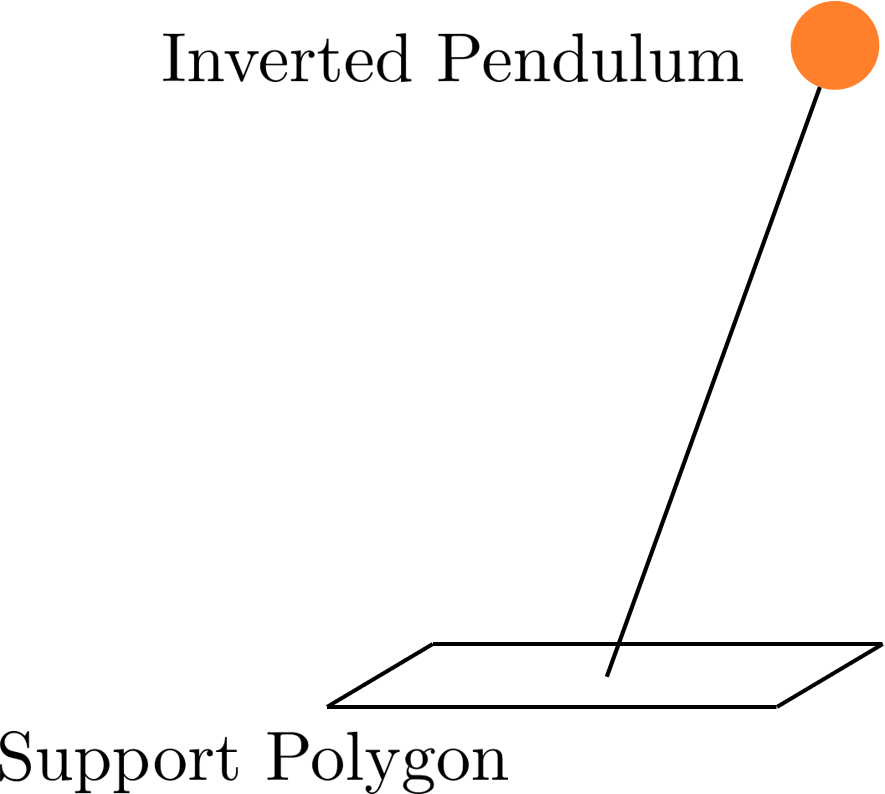
\includegraphics[scale=.3]{chapters/03_background/img/inverted_pendulum.png}}
	\subcaptionbox{}%
	[.4\linewidth]{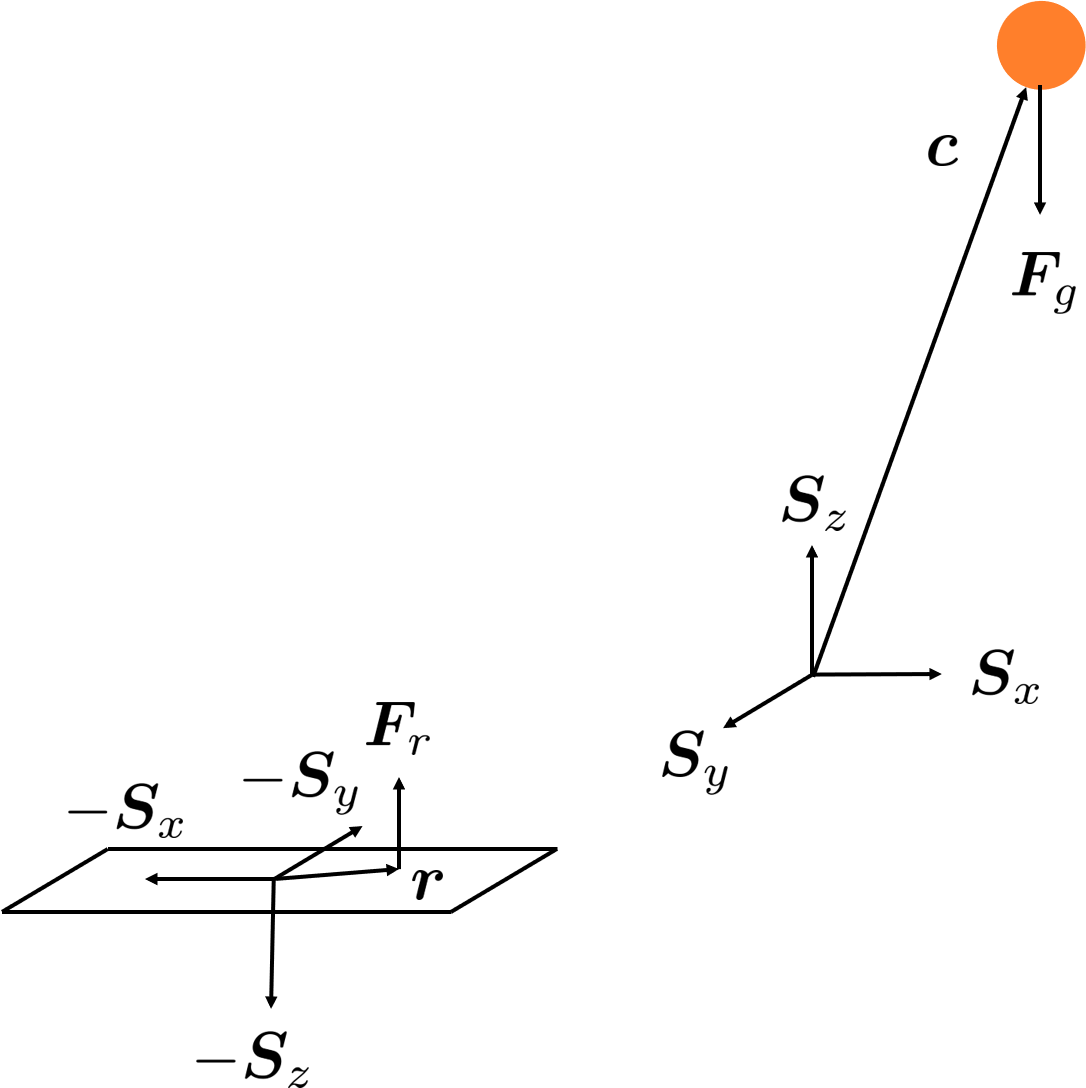
\includegraphics[scale=.3]{chapters/03_background/img/inverted_pendulum_free_body_diagram.png}}
	\caption{Linear inverted pendulum with a support polygon (a), and the corresponding free body diagram with cutting forces $\bm{S}_{x/y/z}$ (b).}
	\label{fig::311_lip}
\end{figure}
The system of interest is shorty depicted in figure \ref{fig::311_lip}. We assume the support polygon of the shown linear inverted pendulum to have zero mass. By introducing cutting forces $\bm{S}_{x/y/z}$ for each degree of freedom in which the motion of the linear inverted pendulum is restricted, we obtain the free body diagram (fig. \ref{fig::311_lip}), for which the acting forces are
\begin{align}
	m\ddot{\bm{c}} &=\quad\bm{S} - \bm{F}_g 
	\label{eq::311_pendulum_force} \\
	\bm{0} &= -\bm{S}+\bm{F}_r
	\label{eq::311_support_polygon_force}
\end{align}
where $\bm{S}=\bm{S}_x+\bm{S}_y+\bm{S}_z$. The respective moments, since we do not take any inertias into account, are given by
\begin{align}
	\bm{0} &= (\bm{0}-\bm{c})\times\bm{S} + \bm{M} 
	\label{eq::311_pendulum_moment}\\	
	\bm{0} &= (\bm{r}-\bm{0})\times\bm{F}_r - \bm{M}
	\label{eq::311_support_polygon_moment}	
\end{align}
where the transfer of the moment $\bm{M}$ may for example be induced by friction. If we replace $\bm{S}=\bm{F}_r$ from eq. \ref{eq::311_support_polygon_force}, equations \ref{eq::311_pendulum_moment} and \ref{eq::311_support_polygon_moment} yield 
\begin{align}
	\bm{0} = (\bm{r}-\bm{c})\times\bm{S} = \begin{pmatrix}
	\quad(r_y - c_y)S_z - (r_z - c_z)S_y \\
	-(r_x - c_x)S_z + (r_z - c_z)S_x \\
	\quad(r_x - c_x)S_y - (r_y - c_y)S_x
	\end{pmatrix}
	\label{eq::311_momentum_transfer}
\end{align}
Since our goal is to have a robot that does not fall, we want to achieve that the acceleration along the z-axis becomes zero, hence $\ddot{c}_z=0$. Given this assumption, we can infer from eq. \ref{eq::311_pendulum_force} that $S_z=mg$, as well as $S_x = \ddot{c}_xm$, and $S_y = \ddot{c}_ym$. Furthermore, our foot shall not lift off the floor, and therefore we have $r_z=0$. If we take these assumptions and plug them into the first to rows of eq. \ref{eq::311_momentum_transfer}, we find
\begin{align}
	r_x &= c_x - c_z\frac{\ddot{c}_x}{g}\\
	r_y &= c_y - c_z\frac{\ddot{c}_y}{g}
	\label{eq::311_zmp}
\end{align}
Therein, $r_x$, and $r_y$ are the x-, and y-coordinates of the zero moment point, given the assumption of a linear inverted pendulum. We can see that the position if dependent on the height of the point mass, which is in turn dependent on the robot. The specific values can be set in the configurations file (\href{https://github.com/mhubii/nmpc_pattern_generator/blob/bc79a6d4f9bcfd3794146355af44429f5b7a9fe0/libs/pattern_generator/configs.yaml#L27}{link}).
\\\\
We have now found a simple analytic expression for the relationship of the zero moment point and the center of mass, which will help us to formulate an optimal control problem that we can solve in real time. This simplification is of course only true to some extend, and we need to find a way to verify its accuracy. The easiest way to do so is to measure the real zero moment point. We will further elaborate on this within the next paragraph - Measurement of the Zero Moment Point, and we will derive a method that only relies on force torque sensors in the ankle.
\subsubsection{Measurement of the Zero Moment Point}
There are several methods that enable us to measure the position of the zero moment point, among them the utilization of pressure sensitive soles, as outlined in \cite{kajita2014introduction}. Furthermore, there exist approximate approaches that involve the knowledge of all acting external forces \cite{huang2001planning}, which can for example be obtained from unconstrained inverse dynamics \cite{michel2017dynamic}. Since we can rely on measurements of force torque sensors that are located at the ankles, we will infer the position of the zero moment point from them \cite{kajita2014introduction}. If we consider the force torque sensor to be located a position $\bm{p}_i$ (fig. \ref{fig::311_force_torque}), then we can obtain the moment about any point $\bm{p}$ according to eq. \ref{eq::311_moment}.
\begin{align}
	\bm{\tau}(\bm{p}) = (\bm{p}_i-\bm{p})\times \bm{f}_i + \bm{\tau}_i
	\label{eq::311_moment}
\end{align}
by definition, the moment about the zero moment point vanishes along the horizontal axes, therefore we can then set $\tau_x = \tau_y = 0$ in eq. \ref{eq::311_moment} and then solve for the position to obtain the zero moment point (eq. \ref{eq::311_x_pos_zmp} and \ref{eq::311_y_pos_zmp}).
\begin{align}
	p_x &= \frac{\left[-\tau_{i,y}-(p_{i,z}-p_z)f_{i,x}+p_{i,x}f_{i,z}\right]}{f_{i,z}}
	\label{eq::311_x_pos_zmp}\\
	p_y &= \frac{\left[-\tau_{i,x}-(p_{i,z}-p_z)f_{i,y}+p_{i,y}f_{i,z}\right]}{f_{i,z}}
	\label{eq::311_y_pos_zmp}
\end{align}
If we further choose our coordinate system to lie along the z-axis of the force torque sensor (fig. ...), we can simplify equations \ref{eq::311_x_pos_zmp} and \ref{eq::311_y_pos_zmp} to find
\begin{align}
	p_x &= \frac{(-\tau_{i,y}-f_{1,x}d)}{f_{1,z}} 
	\label{eq::311_x_pos_zmp_simp}\\
	p_y &= \frac{(\tau_{i,x}-f_{1,y}d)}{f_{1,z}}
	\label{eq::311_y_pos_zmp_simp}
\end{align}
We can use equations \ref{eq::311_x_pos_zmp_simp} and \ref{eq::311_y_pos_zmp_simp} to determine the position of the zero moment point for the left and the right foot with respect to coordinates frames that are attached to the respective foot. These circumstances change once not only one, but both feet are in contact with the ground. What still holds true, in the case of a dynamically balanced gait, is the fact that the positions which we just obtained from equations \ref{eq::311_x_pos_zmp_simp} and \ref{eq::311_y_pos_zmp_simp} represent points where the interaction of the robot with the environment can solely be described by a single force along the z-axis. All other forces or torques cancel out. Therefore, to determine the position of the zero moment point for the double support phase, we need to modify equation \ref{eq::311_moment} slightly. This yields 
\begin{align}
	\bm{\tau}(\bm{p}) = \sum_{i\in\{L, R\}} (\bm{p}_i - \bm{p})\times\bm{f}_i
	\label{eq::311_moment_ds}
\end{align}
where the individual torques are now zero and the only forces $\bm{f}_i$ that exist between the robot and the environment can be described by the z-component which are measured at the ankles' force torque sensors. Yet again, to obtain the position of the zero moment point, we have to set the x-, and y-components of the torque in equation \ref{eq::311_moment_ds} to zero and find
\begin{align}
	p_x &= \frac{\sum_{i\in\{L, R\}}p_{i,x}f_{i,z}}{\sum_{i\in\{L, R\}}f_{i,z}} \\
	p_y &= \frac{\sum_{i\in\{L, R\}}p_{i,y}f_{i,z}}{\sum_{i\in\{L, R\}}f_{i,z}}
\end{align}
These expressions of course only hold true in a shared coordinate system and therefore we need to transform the position of the zero moment point which we obtained from equations \ref{eq::311_x_pos_zmp_simp} and \ref{eq::311_y_pos_zmp_simp} to the world frame. Finally, we can write down the formulation for the zero moment point which holds equally true for the single and double support phase
\begin{align}
	p_x &= \frac{p_{R,x}f_{R,z}+p_{L,x}f_{L,z}}{f_{R,z}+f_{L,z}}  \\
	p_y &= \frac{p_{R,y}f_{R,z}+p_{L,y}f_{L,z}}{f_{R,z}+f_{L,z}}
\end{align}
At this point we are now equipped with a general understanding for the zero moment point, as well as with the knowledge of simplified models to compute it analytically, and a method to measure it so that we can evaluate the performance of a potential pattern generator which is based upon the zero moment point. Therefore, in the next chapter - Nonlinear Model Predictive Control, we will try to understand a method that allows us to generate dynamically balanced center of mass and feet trajectories, which 
  % zero moment point
  \subsection{Nonlinear Model Predictive Control}
\label{sec::312_nmpc}
At the heart of nonlinear model predictive control stands sequential quadratic programming. Before we come to the actual problem formulation, we need to understand how sequential quadratic programming can be used to solve nonlinear optimization problems. We will then come to recognize that if we can find a canonical formulation of our problem, it will become possible to apply sequential quadratic programming to it. The next paragraph - Sequential Quadratic Programming, will therefore shortly introduce the reader to the desired method that will be used to solve the  nonlinear optimization problem, while the subsequent paragraph - Canonical Formulation of Nonlinear Model Predictive Control, will then explain how to fit humanoid walking into this framework.
\subsubsection{Sequential Quadratic Programming}
Sequential quadratic programming is a powerful concept to solve nonlinearly constrained optimization problems. The nonlinear programming problem to be solved is of the form
\begin{align}
	\min_{\bm{x}}\, &f(\bm{x})\\
	\text{subject to: } &\bm{h}(\bm{x}) = \bm{0}\\
	&\bm{g}(\bm{x}) \leq \bm{0},
\end{align}
where $f:\,\mathcal{R}^N\rightarrow\mathcal{R}$, $\bm{h}:\,\mathcal{R}^N\rightarrow\mathcal{R}^M$, and $\bm{g}:\,\mathcal{R}^N\rightarrow\mathcal{R}^P$ \cite{boggs1995sequential}. These problems arise in a variety of applications in science and include quadratic problems as special cases. The great strength of sequential quadratic programming is its ability to solve problems with nonlinear constraints, and its basic idea is to model nonlinear programming at an approximate solution $\bm{x}_k$ by a quadratic subproblem, so to find a solution to this subproblem, in order to construct a better approximation $\bm{x}_{k+1}$. Now given an objective function $f(\bm{x})$ represents a sum of squares, the problem at hand turns into a nonlinear least squares problem, and the minimization can be expressed in terms of a Gauss-Newton method \cite{schittkowski1988solving}. That is, given an objective function $f(\bm{x}) = \frac{1}{2}\bm{F}(\bm{x})^T\bm{F}(\bm{x})$, where $\bm{F}=\left(f_1,...,f_l\right)^T$, we can apply a quasi Gauss-Newton method as follows
\begin{align}
	\nabla^2f(\bm{x})\Delta\bm{x} + \nabla f(\bm{x}) = 0,
	\label{eq::312_quasi_gn}
\end{align}
where the gradient and the Hessian matrix are given as
\begin{align}
	\nabla f(\bm{x}) &= \nabla \bm{F}(\bm{x})\bm{F}(\bm{x}) \\
	\nabla^2 f(\bm{x}) &= \nabla \bm{F}(\bm{x})\nabla\bm{F}(\bm{x})^T + \bm{B}(\bm{x}).
\end{align}
Therein, $\bm{B}(\bm{x}) = \sum_1^lf_i(\bm{x})\nabla^2f_i(\bm{x})$. If we are now sufficiently close to an optimal solution $\bm{x}^*$, such that $\bm{F}(\bm{x}^*) = \left(f_1(\bm{x}^*),...,f_l(\bm{x}^*)\right)^T=\bm{0}$, we can neglect $\bm{B}(\bm{x^*})$, which turns equation \ref{eq::312_quasi_gn} into the previously stated Gauss-Newton minimization problem
\begin{align}
	\min_{\Delta\bm{x}}\,||\nabla\bm{F}(\bm{x_k})^T\Delta\bm{x}+\bm{F}(\bm{x}_k)||,
\end{align}
where a new iterate is obtained by $\bm{x}_{k+1}=\bm{x}_k + \alpha_k\Delta \bm{x}$ with an appropriate step length parameter $\alpha_k$. The presented approach assures quadratic convergence, when starting sufficiently close to an optimal solution. Within the next section, we will understand how to apply this concept to control the zero moment point of a linear inverted pendulum in a balanced manner.
\subsubsection{Canonical Formulation of Nonlinear Model Predictive Control}
\cite{kajita2003biped} % original mpc
\cite{herdt2010online} % herdt
\cite{herdt2010walking} % walking without thinking
\cite{naveau2016reactive} % nmpc % nonlinear model predictive control
  \subsection{Interpolating Trajectories}
\label{sec::313_it}
As already shortly depicted in figure \ref{fig::31_pg}, we need to interpolate the trajectories that we obtain from the nonlinear model predictive control. This especially holds true for the feet, since the computed results do only consider the pendulums dynamic balance with respect to the x-, and the y-position, but not with respect to a robot that has to lift its feet along the z-axis. Furthermore, the feet's movement shall be executed such they stop moving when they are about to touch the ground. This constraint, and others, will be achieved by interpolating the feet trajectories with polynomials. In order to then match the center of mass trajectory's temporal resolution with the feet trajectories', we will upscale it under the already well known assumption of a linear inverted pendulum. The resulting trajectories are shown in figure \ref{fig::313_ip}, and will further be explained in the following. 
\begin{figure}[h]
	\centering
	\subcaptionbox{}%
	[.4\linewidth]{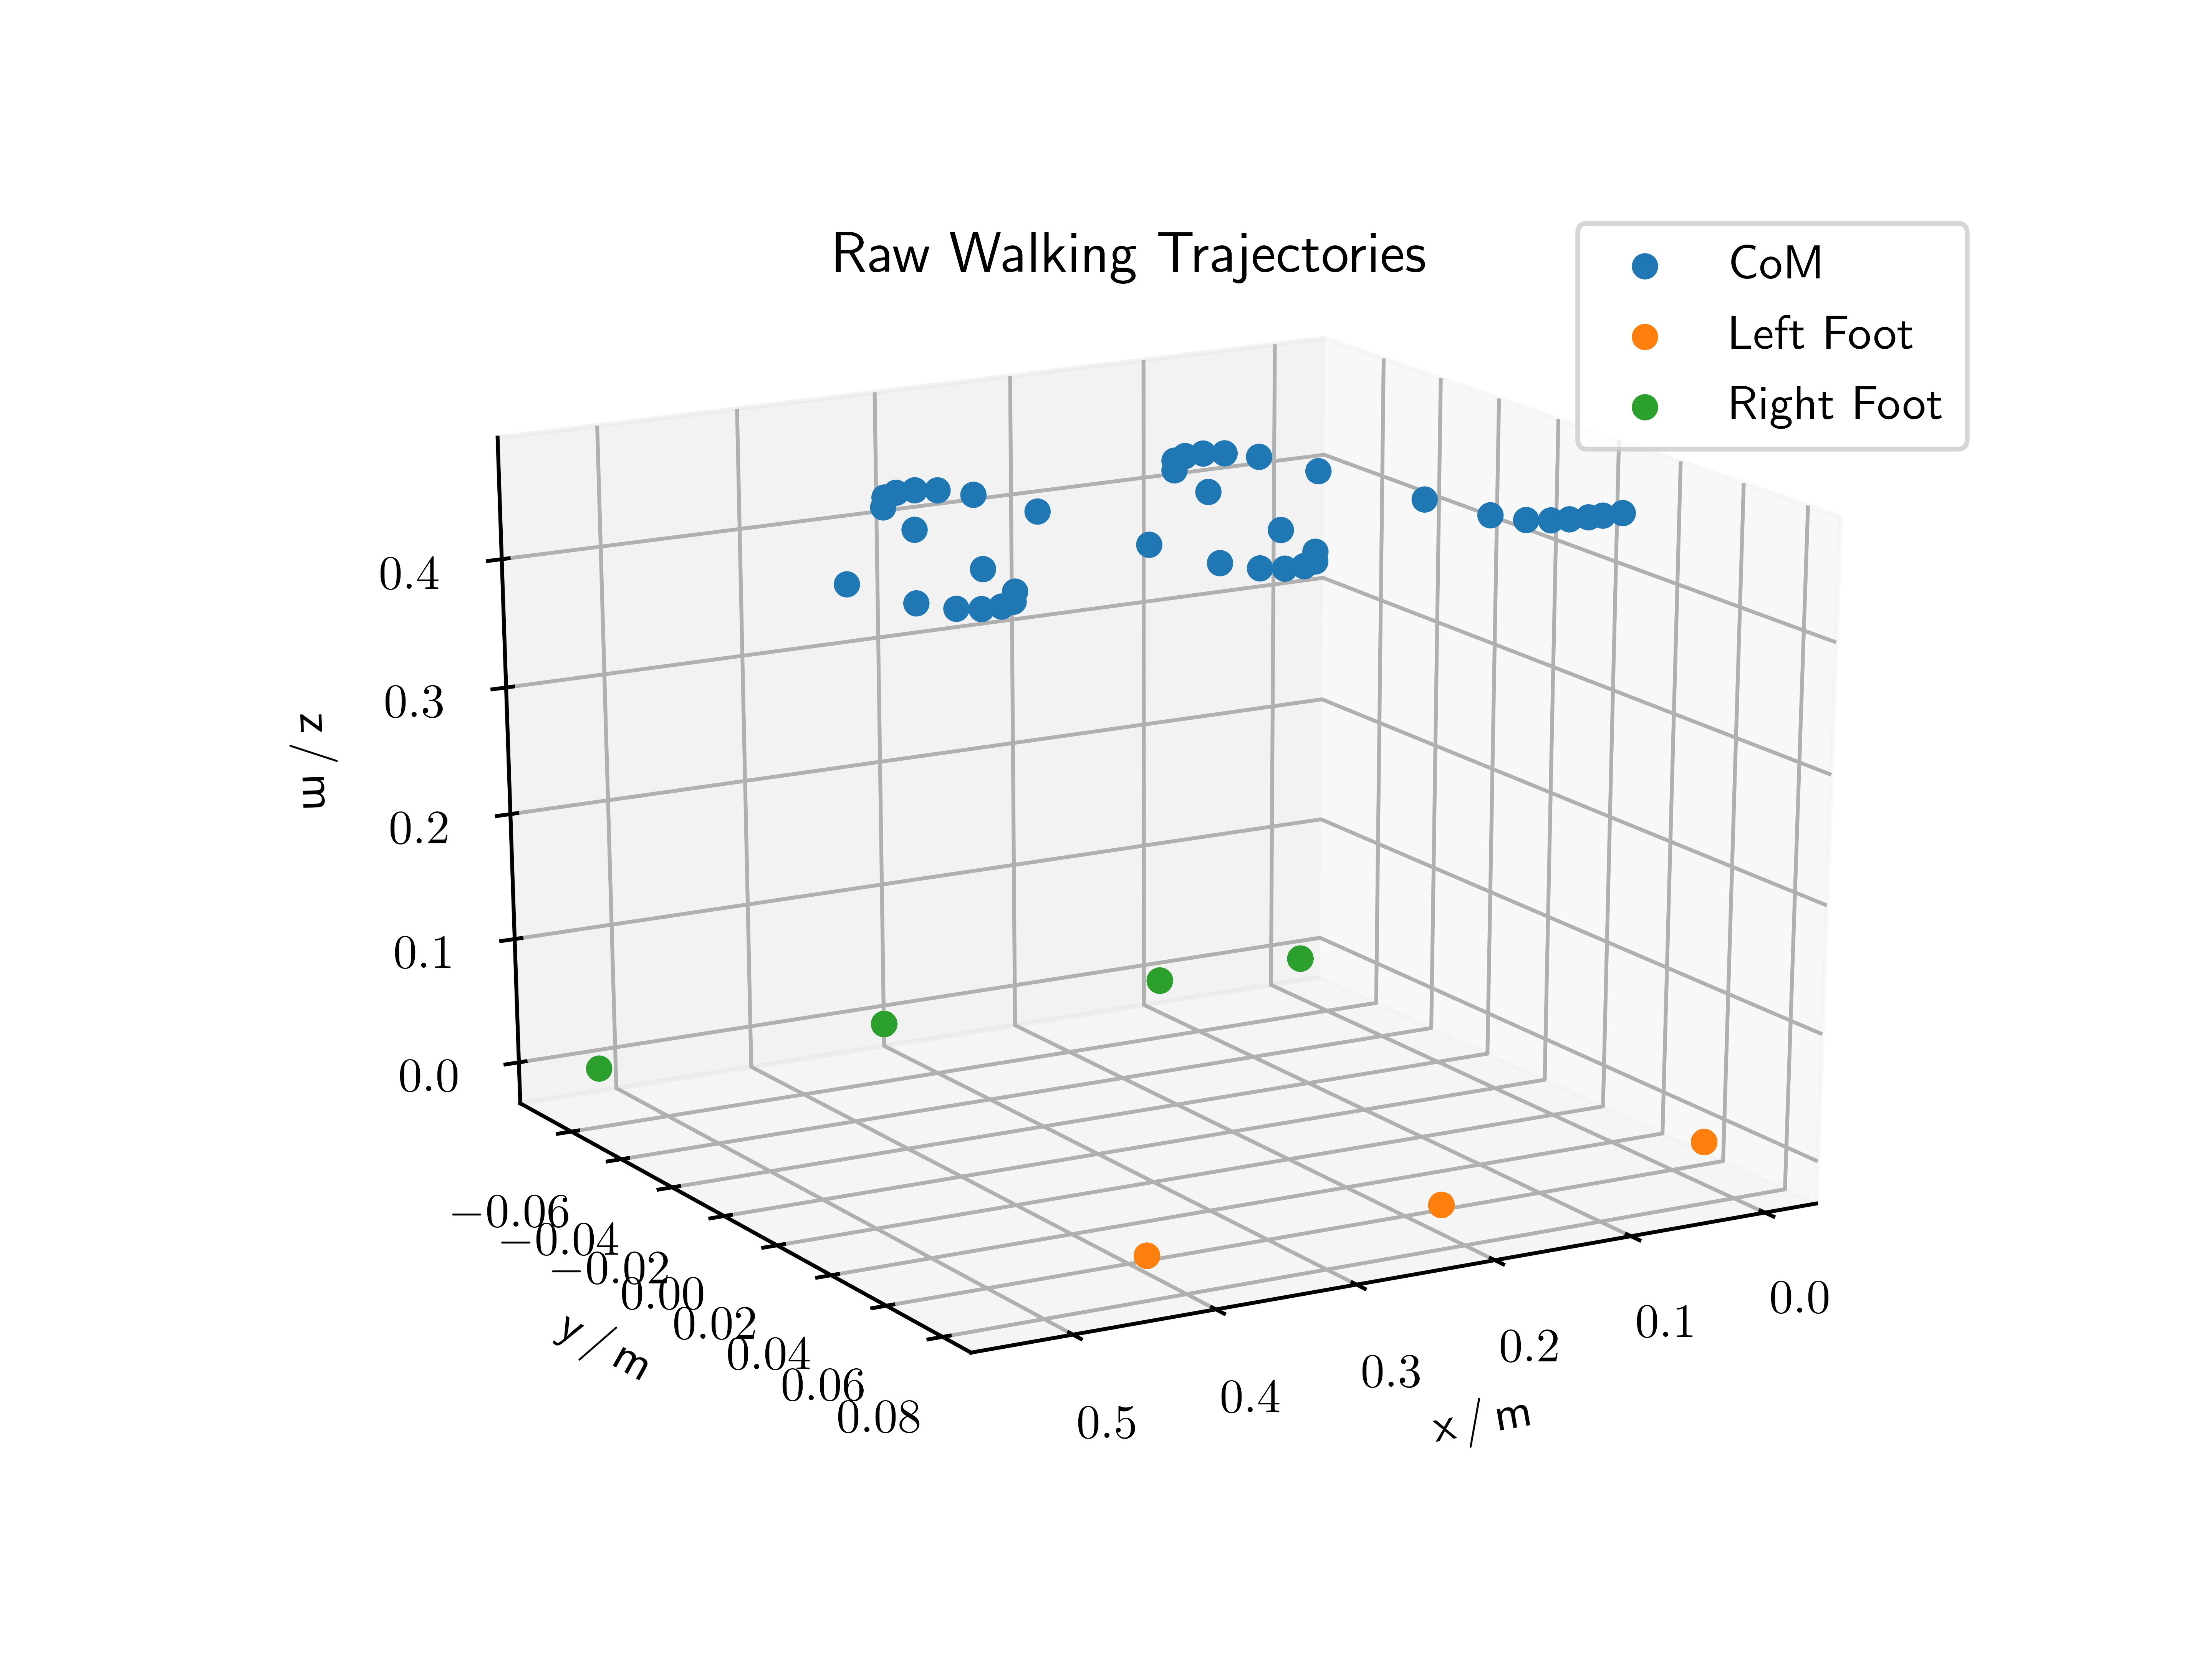
\includegraphics[scale=.4]{chapters/03_background/img/raw_results.png}}
	\subcaptionbox{}%
	[.4\linewidth]{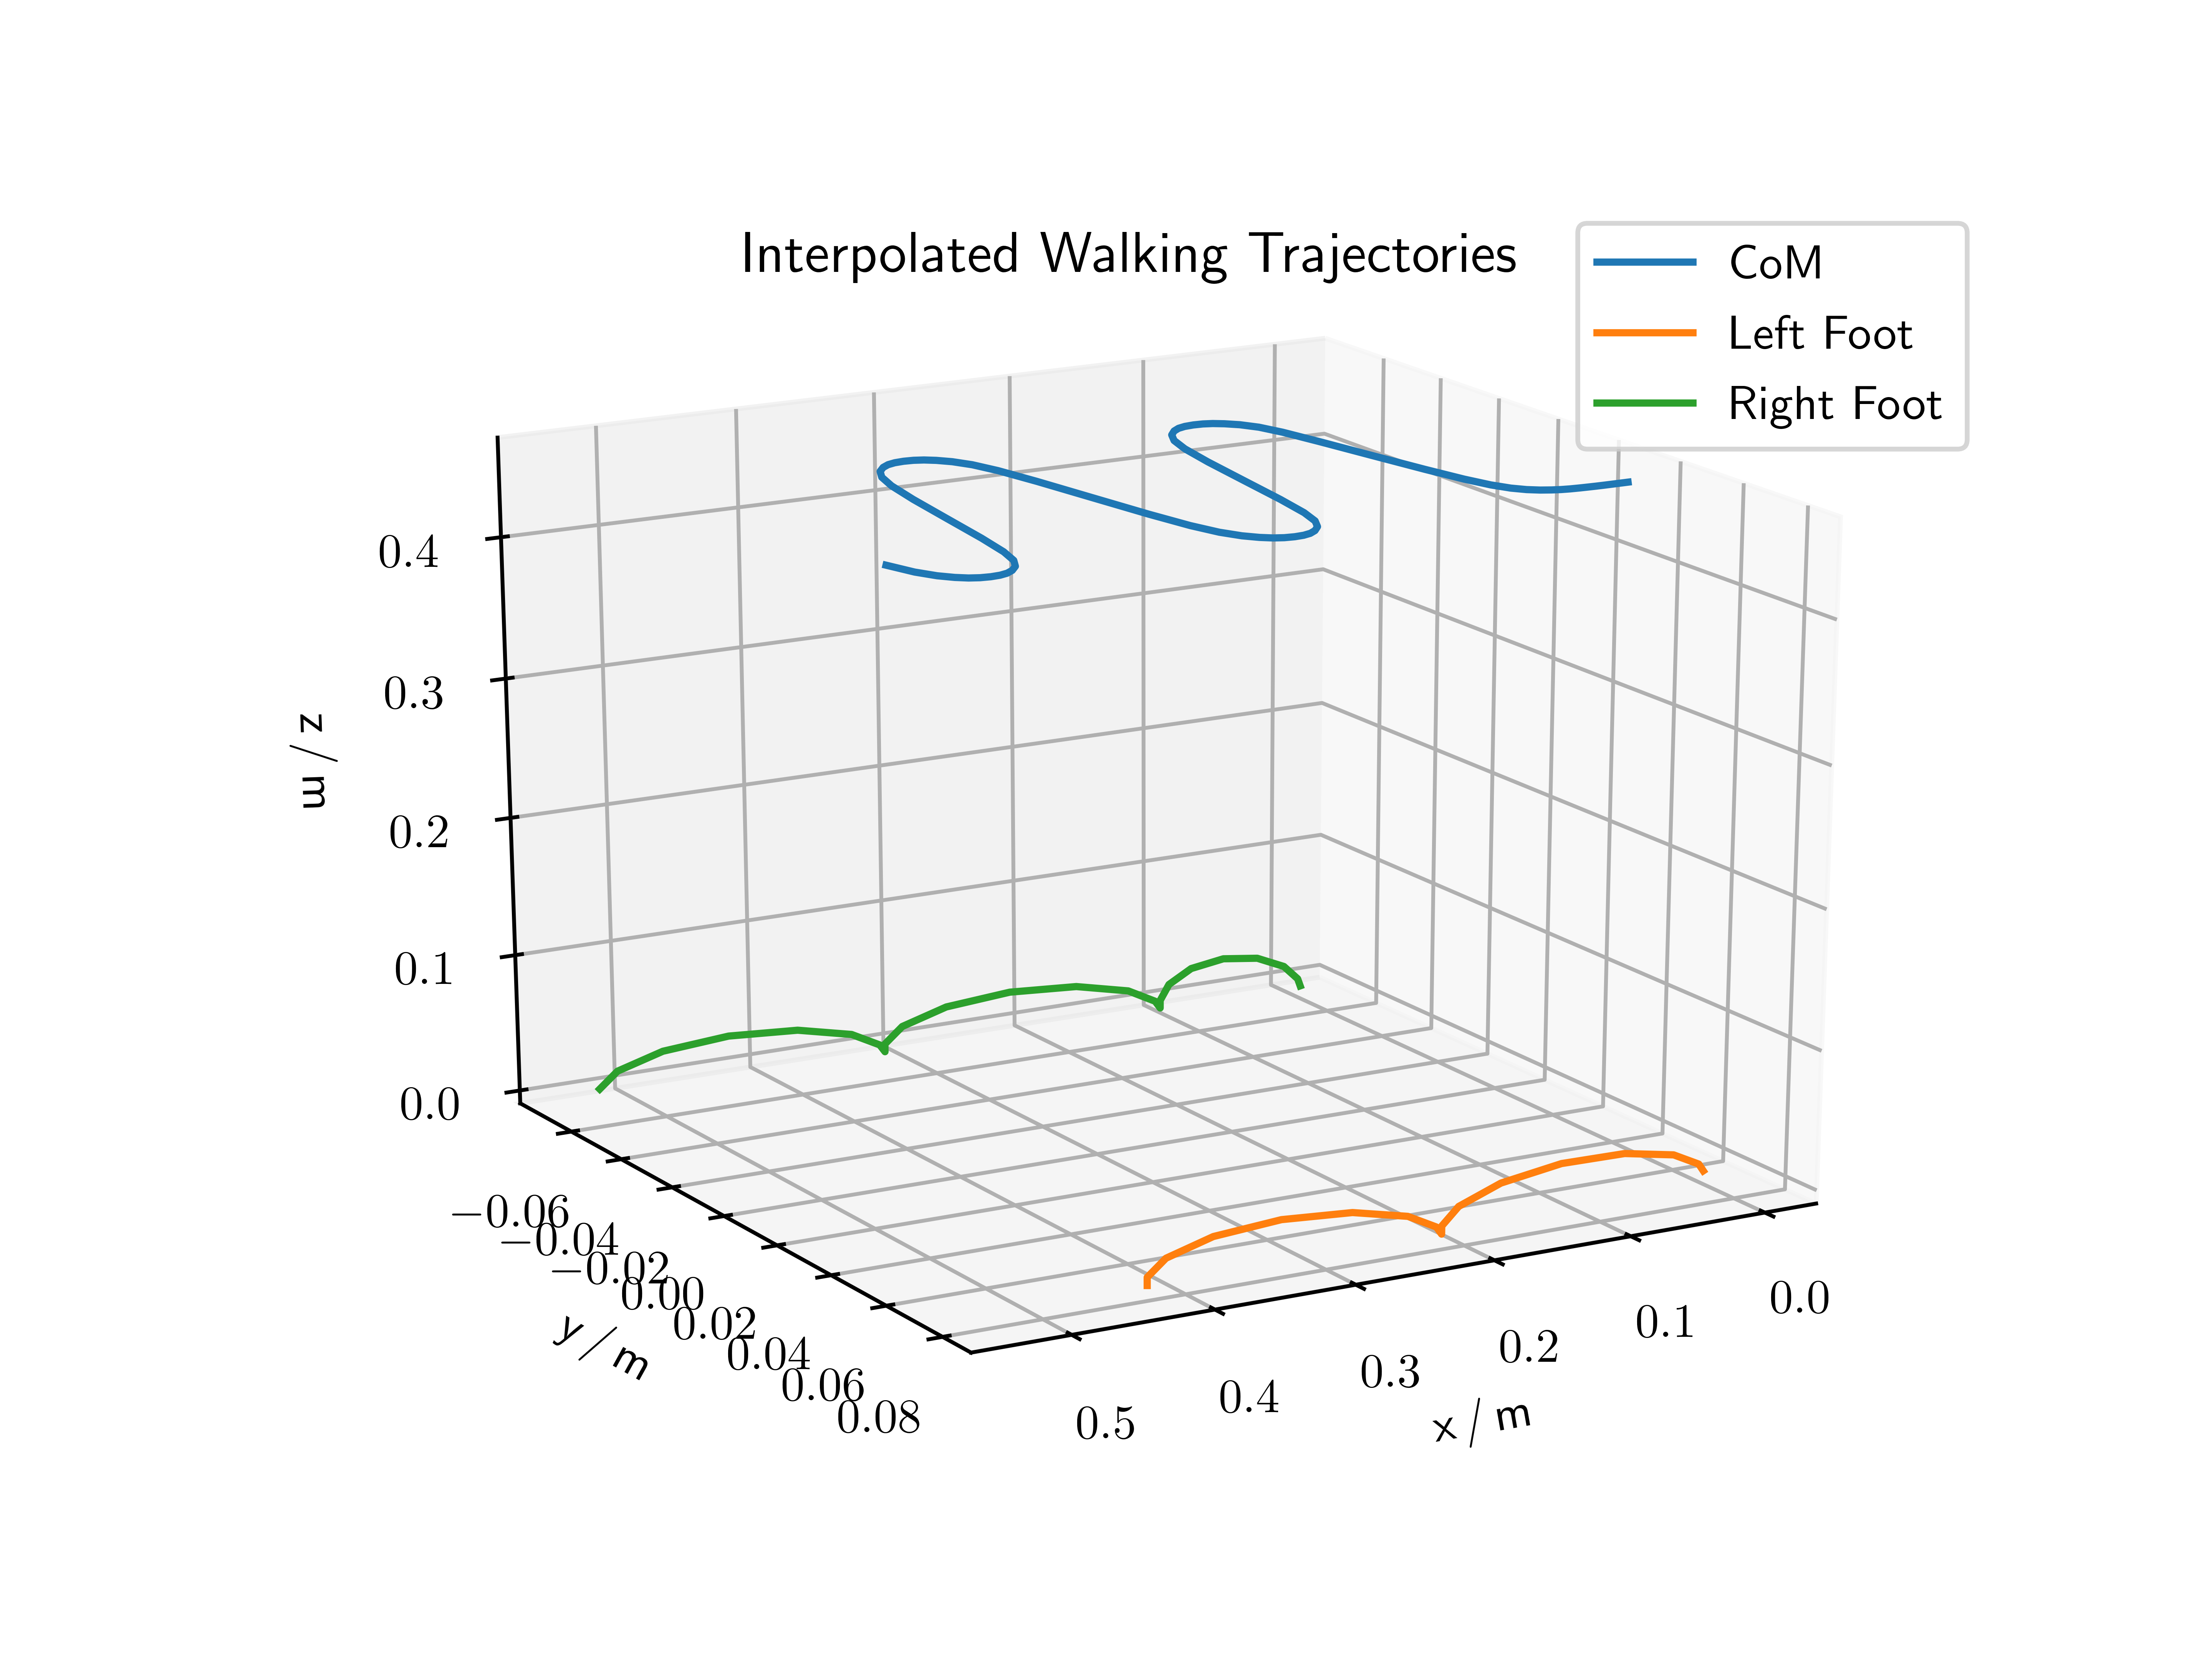
\includegraphics[scale=.4]{chapters/03_background/img/interpolated_results.png}}
	\caption{Uninterpolated trajectories (a), as obtained from the nonlinear model predictive control, and interpolated trajectories (b) for the feet and the center of mass.}
	\label{fig::313_ip}
\end{figure}
\subsubsection{Interpolating the Feet Trajectories}
Any trajectory can in principal be approximated by a polynomial function. For our purposes, we want to approximate positions $p$ as they evolve over time $t$, and further obtain the corresponding velocities $\dot{p}$ and accelerations $\ddot{p}$ (equations \ref{eq::313_pos_poly} - \ref{eq::313_acc_poly}).  
\begin{align}
	p(t) &= \sum_{i = 0}^{N}a_it^i 
	\label{eq::313_pos_poly}\\
	\dot{p}(t) &= \sum_{i = 1}^{N}ia_it^{(i-1)} 
	\label{eq::313_vel_poly}\\
	\ddot{p}(t) &= \sum_{i = 2}^{N}i(i-1)a_it^{(i-2)}
	\label{eq::313_acc_poly}
\end{align}
The coefficients $a_i$ of the polynomials can be chosen such that certain boundary conditions $\bm{b}$ are satisfied. For the lift-off and the drop-down of the robot's feet, these boundary conditions must satisfy a zero initial velocity $\dot{z}_\text{init}$ and a zero end velocity $\dot{z}_\text{end}$, as well as a zero initial height $z_\text{init}$ and a zero end height $z_\text{end}$, and a maximum step height $z_{T/2}$ in between, or else they will hit the ground in an unbalanced way. These conditions are listed below, where each height $z(t)$ and each velocity $\dot{z}(t)$ is written in terms of a polynomial, just as in equations \ref{eq::313_pos_poly} and \ref{eq::313_vel_poly}, respectively. 
\begin{align}
	z(t = 0) &= z_\text{init} = 0
	\label{eq::313_z_bound_1} \\
	\dot{z}(t = 0) &= \dot{z}_\text{init} = 0 \\
	z(t = \frac{T}{2}) &= z_{T/2}\\  
	z(t = T) &= z_\text{end} = 0 \\
	\dot{z}(t = T) &= \dot{z}_\text{end} = 0 
	\label{eq::313_z_bound_5}
\end{align}
To satisfy 5 boundary conditions, it is required to have a polynomial of 4th order with 5 coefficients $a_{z,i}$ in total. In matrix formulation we can express equations \ref{eq::313_z_bound_1} - \ref{eq::313_z_bound_5} as follows
\begin{align}
	\bm{M}_z\bm{a}_z &= \bm{b}_z \\
	\begin{pmatrix}
		1 & 0 & 0              & 0              & 0 \\
		0 & 1 & 0              & 0              & 0 \\
		1 & \left(\frac{T}{2}\right)        & \left(\frac{T}{2}\right)^2  & \left(\frac{T}{2}\right)^3 & \left(\frac{T}{2}\right)^4 \\
		1 & T & T^2            & T^3            & T^4 \\
		0 & 1 & 2T             & 3T^2           & 4T^3 
	\end{pmatrix}
	\begin{pmatrix}
		a_{z,0} \\
		a_{z,1} \\
		a_{z,2} \\
		a_{z,3} \\
		a_{z,4}
	\end{pmatrix} &=
	\begin{pmatrix}
		z_\text{init} \\
		\dot{z}_\text{init} \\
		z_{T/2} \\
		z_\text{end}\\
		\dot{z}_\text{end}
	\end{pmatrix}.
\end{align}
Inversion then yields
\begin{align}
	\bm{a}_z&=\bm{M}_z^{-1}\bm{b}_z \\
	\begin{pmatrix}
		a_{z,0} \\
		a_{z,1} \\
		a_{z,2} \\
		a_{z,3} \\
		a_{z,4}
	\end{pmatrix} &=
	\begin{pmatrix}
		1 & 0 & 0 & 0 & 0 \\
		0 & 1 & 0 & 0 & 0 \\
		-\frac{11}{T^2} & -\frac{4}{T} & \frac{16}{T^2} & -\frac{5}{T^2} & \frac{1}{T} \\
		\frac{18}{T^3} & \frac{5}{T^2} & -\frac{32}{T^3} & \frac{14}{T^3} & -\frac{3}{T^2} \\
		-\frac{8}{T^4} & -\frac{2}{T^3} & \frac{16}{T^4} & -\frac{8}{T^4} & \frac{2}{T^3}
	\end{pmatrix}
	\begin{pmatrix}
		z_\text{init} \\
		\dot{z}_\text{init} \\
		z_{T/2} \\
		z_\text{end}\\
		\dot{z}_\text{end}
	\end{pmatrix}.
\end{align}
The obtained coefficients $a_i$ are then used to compute the height of each foot during a single support phase (\href{https://github.com/mhubii/nmpc_pattern_generator/blob/c82c64a28da7527e75442764f585bd50a8f61ee9/libs/pattern_generator/src/interpolation.cpp#L779}{link}). The maximum step height $z_{T/2}$ (\href{https://github.com/mhubii/nmpc_pattern_generator/blob/c82c64a28da7527e75442764f585bd50a8f61ee9/libs/pattern_generator/configs.yaml#L22}{link}), and the single support time $T$ (\href{https://github.com/mhubii/nmpc_pattern_generator/blob/c82c64a28da7527e75442764f585bd50a8f61ee9/libs/pattern_generator/configs.yaml#L21}{link}), which is the step time minus the double support time, can be set in the configurations file. For the x-, and the y-positions of the feet, we can define boundary conditions in a similar fashion. In contrary to the computation of the z-position, the x-, and the y-position interpolation of the feet allows for feedback. Therefore, we require additional constraints that satisfy the accelerations as follows
\begin{align}
	x(t = 0) &= x_\text{init} 
	\label{eq::313_x_bound_1}\\
	\dot{x}(t=0) &= \dot{x}_\text{init} \\
	\ddot{x}(t=0) &= \ddot{x}_\text{init} \\
	x(t=T) &= x_\text{end}\\
	\dot{x}(t=T) &= \dot{x}_\text{end} \\
	\ddot{x}(t=T) &= \ddot{x}_\text{end}.
	\label{eq::313_x_bound_6}
\end{align}
Again, we can rewrite equations \ref{eq::313_x_bound_1} - \ref{eq::313_x_bound_6} in matrix formulation
\begin{align}
	\bm{M}_x\bm{a}_x &= \bm{b}_x \\
	\begin{pmatrix}
		1 & 0 & 0 & 0 & 0 & 0 \\
		0 & 1 & 0 & 0 & 0 & 0 \\
		0 & 0 & 2 & 0 & 0 & 0 \\
		1 & T & T^2 & T^3 & T^4 & T^5 \\
		0 & 1 & 2 T & 3 T^2 & 4 T^3 & 5 T^4 \\
		0 & 0 & 2 & 6 T & 12 T^2 & 20 T^3
	\end{pmatrix}
	\begin{pmatrix}
		a_{x,0} \\
		a_{x,1} \\
		a_{x,2} \\
		a_{x,3} \\
		a_{x,4} \\
		a_{x,5}
	\end{pmatrix} &=
	\begin{pmatrix}
		x_\text{init} \\
		\dot{x}_\text{init} \\
		\ddot{x}_\text{init} \\
		x_\text{end} \\
		\dot{x}_\text{end} \\
		\ddot{x}_\text{end} 
	\end{pmatrix},
\end{align}
and inversion yields the polynomial's coefficients $a_{x,i}$
\begin{align}
	\bm{a}_x &= \bm{M}_x^{-1}\bm{b}_x \\
	\begin{pmatrix}
		a_{x,0} \\
		a_{x,1} \\
		a_{x,2} \\
		a_{x,3} \\
		a_{x,4} \\
		a_{x,5}
	\end{pmatrix} &= 
	\frac{1}{2}
	\begin{pmatrix}
		2 & 0 & 0 & 0 & 0 & 0 \\
		0 & 2 & 0 & 0 & 0 & 0 \\
		0 & 0 & 1 & 0 & 0 & 0 \\
		-\frac{20}{T^3} & -\frac{12}{T^2} & -\frac{3}{T} & \frac{20}{T^3} & -\frac{8}{T^2} & \frac{1}{T} \\
		\frac{30}{T^4} & \frac{16}{T^3} & \frac{3}{T^2} & -\frac{30}{T^4} & \frac{14}{T^3} & -\frac{2}{T^2} \\
		-\frac{12}{T^5} & -\frac{6}{T^4} & -\frac{1}{T^3} & \frac{12}{T^5} & -\frac{6}{T^4} & \frac{1}{T^3} \\
	\end{pmatrix}
	\begin{pmatrix}
		x_\text{init} \\
		\dot{x}_\text{init} \\
		\ddot{x}_\text{init} \\
		x_\text{end} \\
		\dot{x}_\text{end} \\
		\ddot{x}_\text{end} 
	\end{pmatrix}.
\end{align}
The exact same formalism is used to interpolate the foot's y-position during single support phase (\href{https://github.com/mhubii/nmpc_pattern_generator/blob/c82c64a28da7527e75442764f585bd50a8f61ee9/libs/pattern_generator/src/interpolation.cpp#L806}{link}). In contrast to the interpolation of the feet's positions, the center of mass positions will be extrapolated under the introduced assumption of a linear inverted pendulum. The method will be shortly explained in the following paragraph - Interpolating the Center of Mass Trajectories.
\subsubsection{Interpolating the Center of Mass Trajectories}
The center of mass trajectories can now simply be adjusted to the temporal resolution of the feet trajectories by applying the linear time stepping scheme from equation \ref{eq::321_ltss} with an adjusted temporal resolution $T$. An iterative application (\href{https://github.com/mhubii/nmpc_pattern_generator/blob/5a213044c927dc6aac9f7e32ce1e5fb472cd67bb/libs/pattern_generator/src/interpolation.cpp#L776}{link}) of these matrices then yields the desired interpolation. The only requirement left to get our robot to walk is now the transformation of trajectories in Cartesian space to trajectories within the joint space, which will be resolved in the following chapter - Kinematics.   % interpolation
  \subsection{Kinematics}
\label{sec::314_k}
\subsubsection{Forward Kinematics}
\label{sec::3141_fk}
\subsubsection{Inverse Kinematics}
\label{sec::3142_ik}   % kinematics
  
  \section{Machine Learning}  
\label{sec::32_ml}
   % short overview of machine learning
  \subsection{Neural Networks}
\label{sec::321_nn}
\subsubsection{Backpropagation}
\subsubsection{Fully Connected Neural Network}
\subsubsection{Convolutional Neural Network}
\subsubsection{Long Short-Term Memory}
\begin{figure}[h]
	\centering
	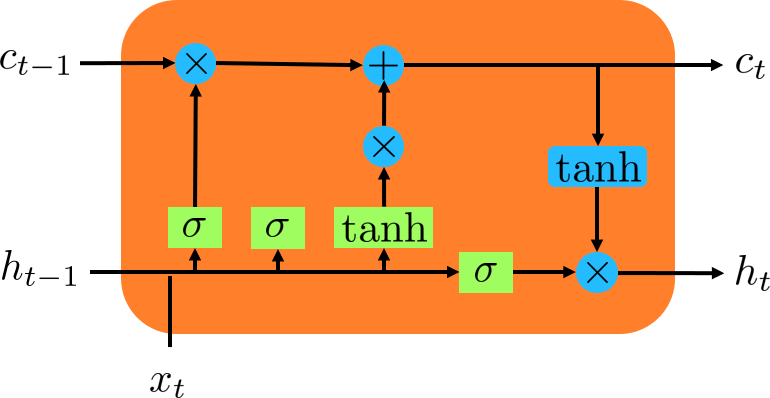
\includegraphics[scale=.5]{chapters/03_background/img/lstm.png}
	\caption{}
	\label{fig::321_lstm}
\end{figure}

   % short introduction to neural networks
  \subsection{Behavioral Cloning}
\label{sec::322_bc}
Behavioral cloning in itself is not always related to machine learning, but poses one possible way of training a neural net in a supervised manner. The presented concept is easy to understand and got inspired by \cite{bojarski2016end}, where it was used for self-driving cars, and since having a car drive along the road is easier to achieve than having a robot walk around an environment, we will deal with the additional details later to focus on the main points for now. The proposed method utilizes the control loop, which was already introduced in figure \ref{fig::3_cl}. In order to then replace the human user by an artificial agent, we have a human user perform a desired behavior, and copy it. The required extended control loop is shown in figure \ref{fig::322_bc}.
\begin{figure}[h]
	\centering
	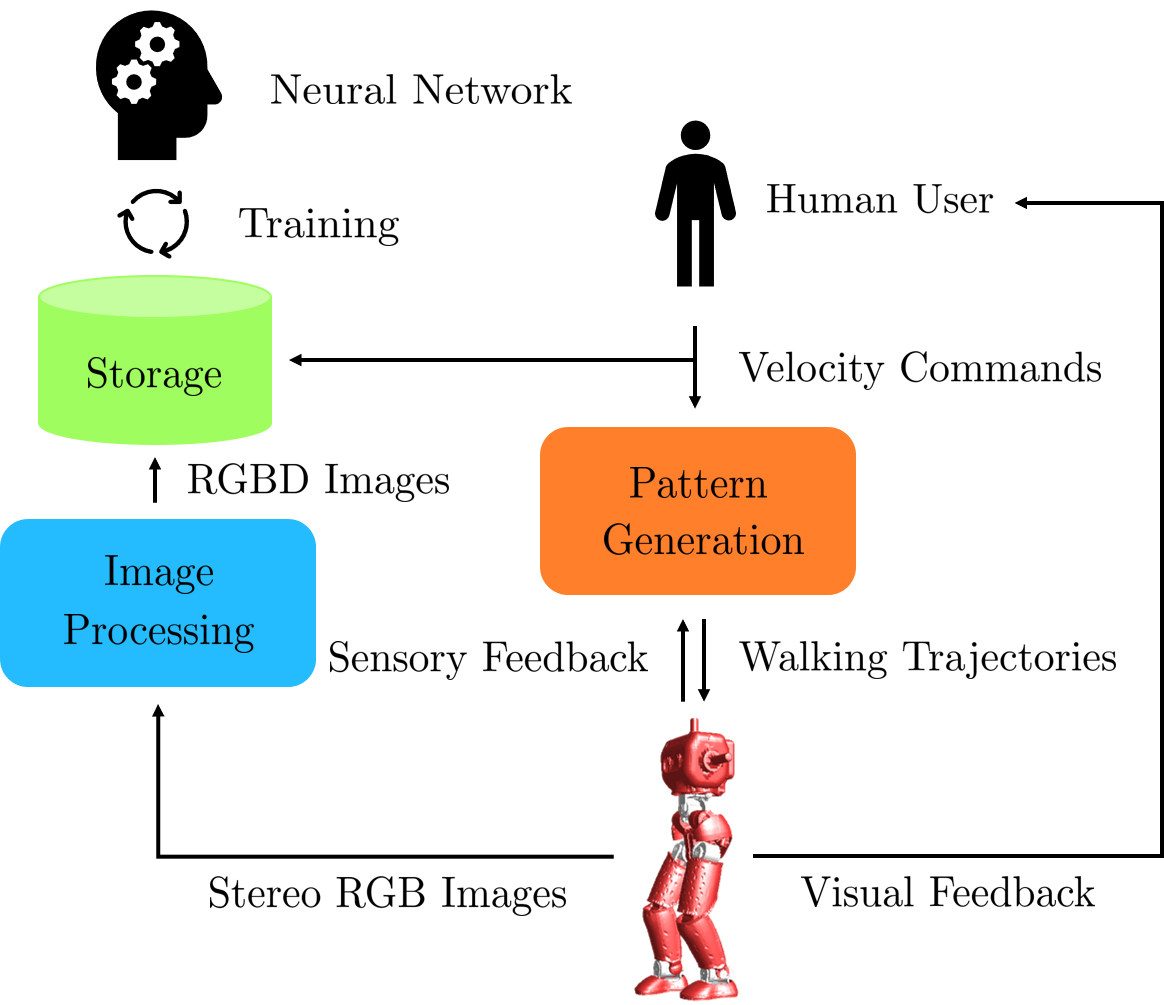
\includegraphics[scale=.5]{chapters/03_background/img/behavioral_cloning.png}
	\caption{Pipeline for behavioral cloning. The neural network is trained on stored RGBD images, and corresponding velocity commands that are correlated by a timestamp}
	\label{fig::322_bc}
\end{figure}
It simply takes the velocity commands from the human user, and stores it alongside RGBD images with a corresponding timestamp to some storage, where the RGBD images are obtained from stereo RGB images by an image processing step that is explained in section \ref{sec::324_ip}. The timestamp allows to correlate seen images to desired velocities afterwards, which in turn enables an artificial agent to train on the stored data. For our purposes, the artificial agent is a neural network. An appropriately chosen network architecture will then enable us to learn the taught behavior and ultimately lets us replace the human user. This procedure relies on prior knowledge to achieve certain tasks, namely the stored data. There are other algorithms that explore the state space on their own, and for which we could for example use the taught behavior as prior as well. These algorithms belong to the class of reinforcement learning methods, and we will have a look at a particular one in the next section. TODO add information about data in bc, amount of data, distribution etc   % behavioral cloning
  \subsection{Reinforcement Learning}
\label{sec::323_rl}
The goal in reinforcement learning is not only to learn actions $a_t$ at time-step $t$, given a state $s_t$, like it is in behavioral cloning, but further to explore actions and states. This is usually performed as shown in figure \ref{fig::323_rl}, where an agent interacts with an environment to receive a reward $r_t$, and also changes the state as cause of its action. Therein, the actions $a_t$ are sampled from a policy $a_t\sim\pi_\theta(a_t|s_t)$ that depends on parameters $\theta$, which for our case are simply the weights of a neural network. 
\begin{figure}[h]
	\centering
	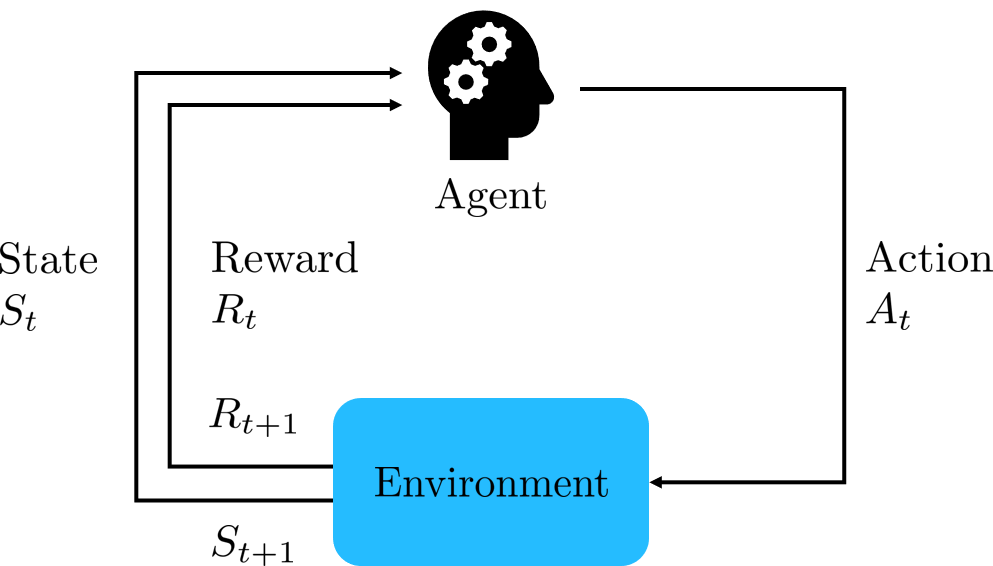
\includegraphics[scale=.5]{chapters/03_background/img/reinforcement_learning.png}
	\caption{Reinforcement learning setup. TODO replace by small letters}
	\label{fig::323_rl}
\end{figure}
The difficulty in optimizing the policy $\pi_\theta$, is to have an agent to discard immediate rewards over future expected rewards. For discrete action spaces, this got well solved by deep Q-learning \cite{mnih2015human}. Different approaches for continuous action spaces like trust region policy optimization \cite{schulman2015trust} are rather complicated. The, to this date, most elegant way of solving continuous control problems in a reinforcement learning setup, is proximal policy optimization \cite{schulman2017proximal}, and we will elaborate on it in the following. Gradient policy methods, such as proximal policy optimization, try to update the policy $\pi_\theta$, such that the expected total future reward $\mathbb{E}\left[\sum_{t=0}^\infty r_t\right]$ is maximized. For the incremental update, it is therefore required to find the gradient of this expression
\begin{align}
	\nabla_\theta\mathbb{E}_{a_t\sim\pi_\theta}\left[\sum_{t=0}^\infty r_t\right] = \mathbb{E}_{a_t\sim\pi_\theta}\left[\sum_{t=0}^\infty\psi_t\nabla_\theta\log\pi_\theta(a_t|s_t)\right],
\end{align}
where $\psi_t$ can take many forms. Since the gradient is just an estimate, as it is computed from samples being taken from the reinforcement learning environment, it usually suffers from variance and bias. As shown in \cite{schulman2015high}, we can trade-off variance for bias and the other way around, by replacing $\psi_t$ for the general advantage estimate $\hat{A}^\text{GAE}_t$ as follows
\begin{align}
	\hat{A}^{\text{GAE}(\gamma,\lambda)}_t = \sum_{l=0}^\infty(\gamma\lambda)^l\delta_{t+l}^V,
	\label{eq::323_gae}
\end{align}
where $\delta^V_{t,l} = r_t + \gamma V(s_{t+1}) - V(s_t)$ is the temporal difference \cite{sutton1998introduction}, and $V$ the value function, which is given by a critic network. The critic's goal then is to have the gradient estimate steer the acting policy network towards actions that maximize the reward. A huge problem therein is that the policy may diverge and that policies may be discarded on the basis of a gradient estimate with a high variance. This is prohibited in proximal policy optimization by clipping the general advantage estimate, and therefore the gradient, under the following objective
\begin{align}
	L^\text{CLIP} = \min(\rho_t(\theta)\hat{A}_t, \text{clip}(\rho_t(\theta), 1-\epsilon, 1+\epsilon)\hat{A}_t),
\end{align}
where $\rho_t(\theta) = \frac{\pi_\theta(a_t|s_t)}{\pi_{\theta_\text{old}}(a_t|s_t)}$ is the probability ratio of the old and the new policy. The loss is shown in figure \ref{fig::323_ppo}, and it assures for a positive advantage estimate that the gradient does not diverge towards actions that are way more likely under the new policy, than they have been for the old policy.
\begin{figure}[h]
	\centering
	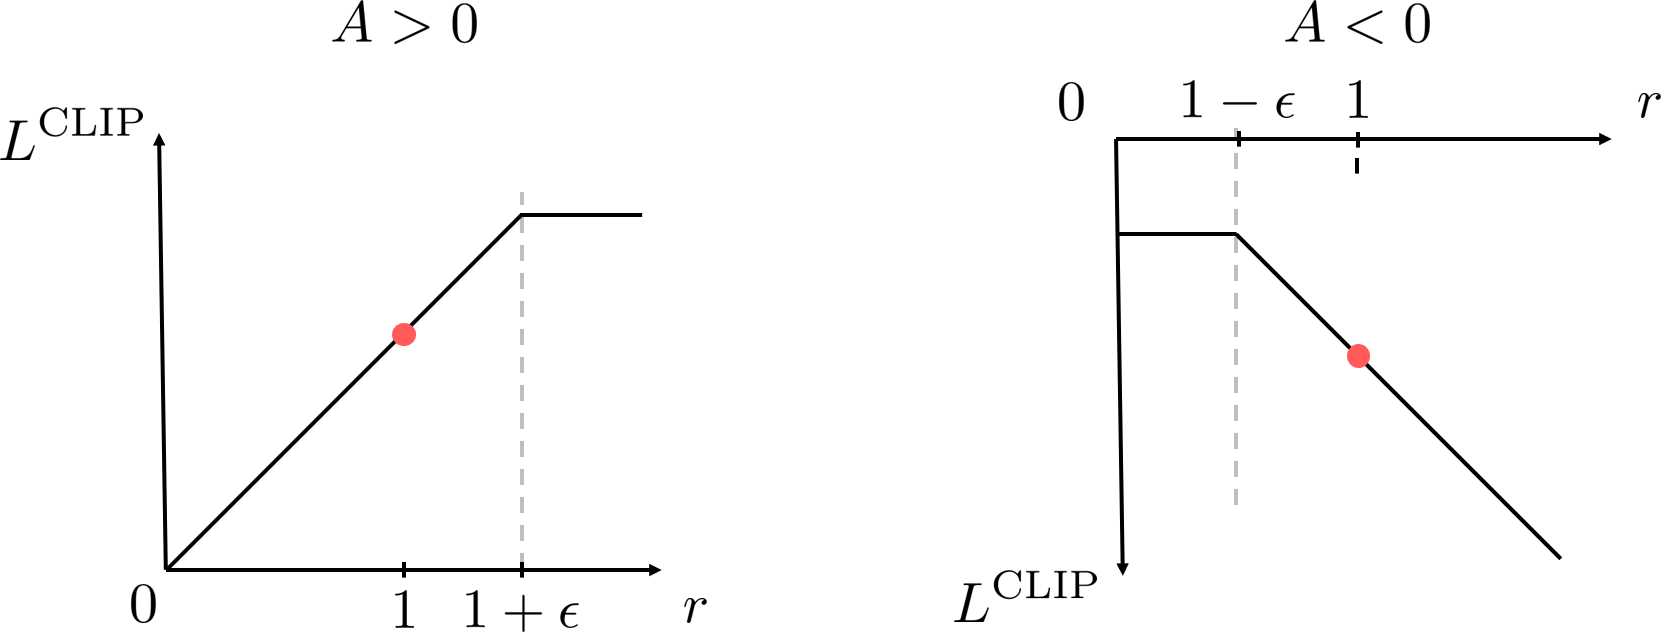
\includegraphics[scale=.35]{chapters/03_background/img/ppo_objective.png}
	\caption{PPO TODO replace A by $\hat{A}_t$ and r by $\rho$}
	\label{fig::323_ppo}
\end{figure}
Also, for a negative advantage estimate, it assures that the gradient points aways from these policies. The total objective $L_t^{\text{CLIP}+\text{VF}+\text{S}}$ of proximal policy optimization is further extended by an entropy term $S$ that results in exploration, and the critic's loss $L^\text{VF}$, such that it can steer the gradient (equation \ref{eq::323_ppo_loss}).
\begin{align}
	L_t^{\text{CLIP}+\text{VF}+\text{S}} = \mathbb{E}\left[L_t^\text{CLIP}(\theta)-c_1L_t^\text{VF}(\theta)+c_2S\left[\pi_\theta\right](s_t)\right]
	\label{eq::323_ppo_loss}
\end{align}
The critic's loss therein is the squared-error of the value function estimate and the explored values $(V_\theta(s_t)-V^\text{target}_t)^2$.
TODO add algorithm?
   % reinforcement learning
  \subsection{Image Processing}
\label{sec::324_ip}
In the previous sections we have learned about two different approaches to train neural nets on solving certain tasks. Although we came to understand that the complexity of the task to be solved correlates strongly with the amount of data at hand, there exist domains from which it is undeniably easier to do so. To equip a neural net with some sort of prior knowledge by switching the domain may therefore not only be highly desirable but sometimes also needed if the amount or quality of data is not sufficient. One domain which is of special interest when it comes to interacting in a three dimensional environment is a domain that represents depth information. If there are any, it may sometimes be possible to extract this kind of prior knowledge from a depth camera. As for this work, we need to rely on stereo cameras and powerful algorithms that allow us to compute depth images in real time. The algorithm that helps us to do so, in terms of the extraction of weighted least squares disparity maps \cite{min2014fast}, will be presented in the following paragraph - Depth Map Extraction.
\subsubsection{Depth Map Extraction}
As already pointed out, the depth map is generated from stereo camera images by a technique called stereo block matching \cite{hamzah2010sum}. This method works best for edge filtered images, as will become clear soon. To obtain edge filtered images $\bm{E}$, the stereo RGB images are first converted into grayscale $\bm{G}$, which are then convolved with the Sobel kernel $\bm{S}_x$ along the horizontal axis \cite{sobel2014an} (equation \ref{eq::324_sobel_conv}, figure \ref{fig::324_image_preprocessing}). 
\begin{align}
	\bm{E} = \bm{S}_x*\bm{G}
	\label{eq::324_sobel_conv}
\end{align}
\begin{figure}[h]
	\centering
	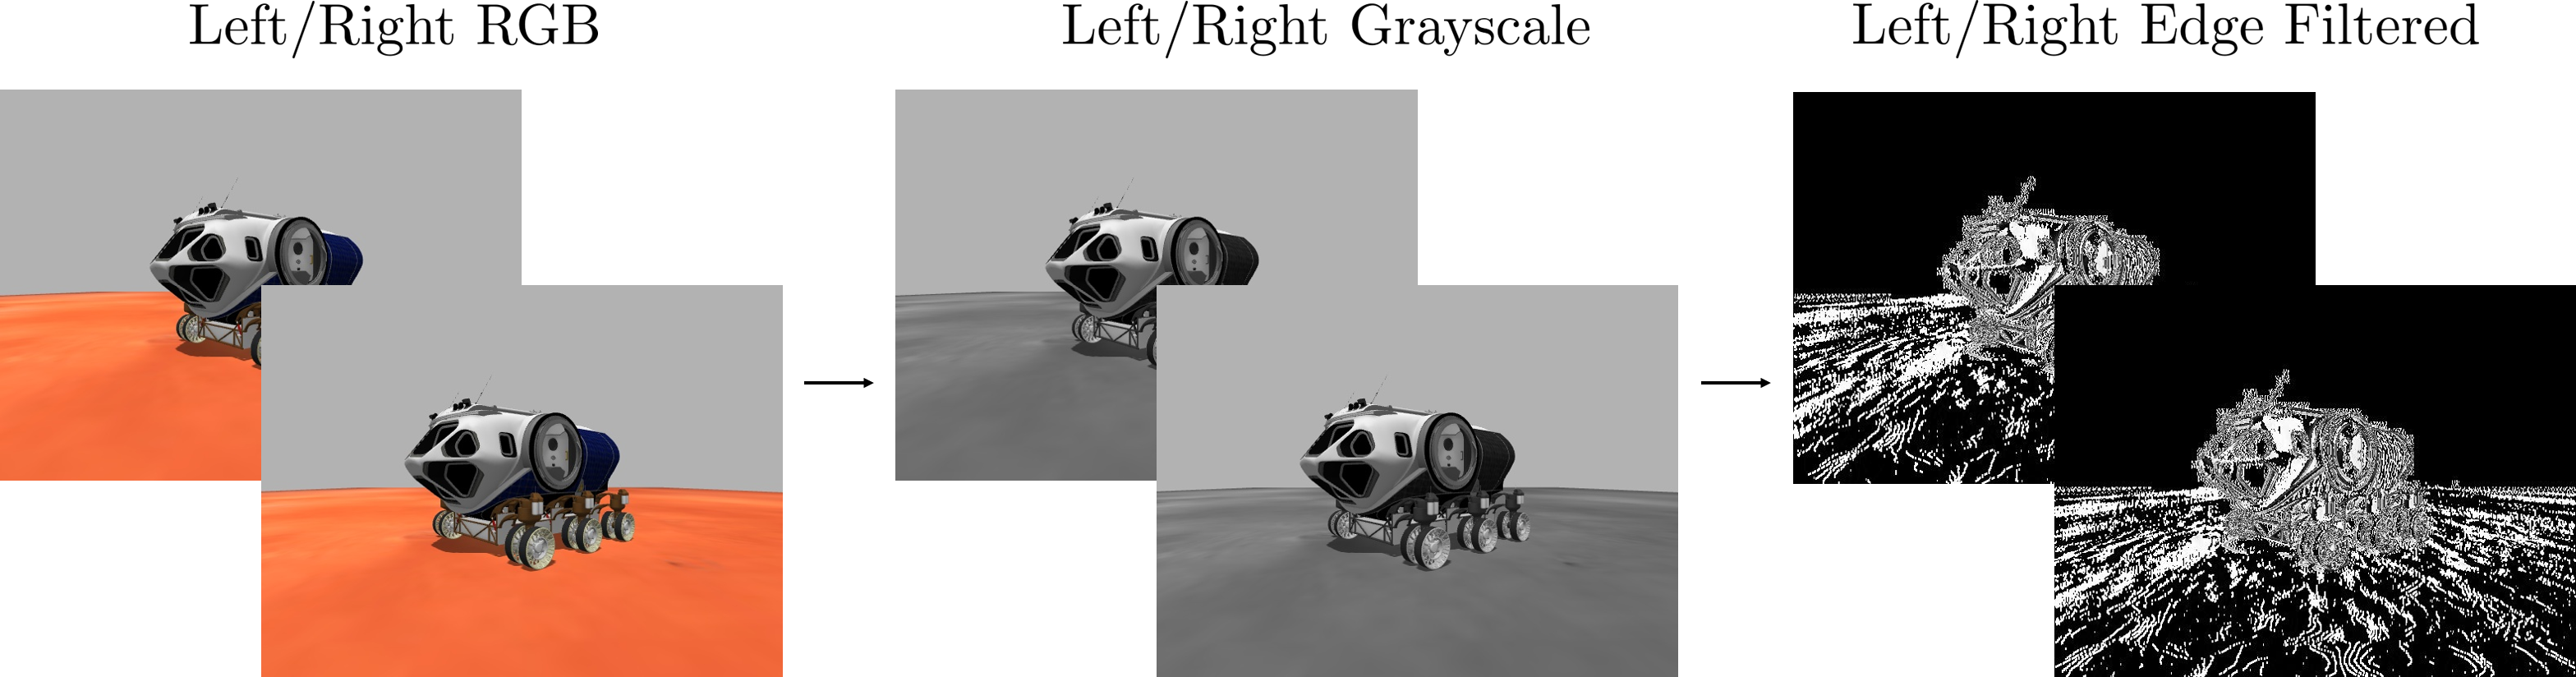
\includegraphics[scale=.28]{chapters/03_background/img/image_preprocessing.png}
	\caption{Image preprocessing to obtain edge filtered images. The images were taken within the simulation environment Gazebo (\href{http://gazebosim.org/}{link}), and show a space exploration vehicle, for which, with the friendly support of NASA, we generated a Gazebo version (\href{https://github.com/mhubii/gazebo_models}{link}).}
	\label{fig::324_image_preprocessing}
\end{figure}
When having a look at the Sobel kernel $\bm{S}_x$ (equation \ref{eq::324_sobel}), it immediately becomes clear that it approximates the derivative of an image along the horizontal axis. Therefore, at locations of steep change, or simply put, edges, the convolution of the grayscale images with the Sobel kernel results in high values, and thus in the typical appearance of an edge filtered image.
\begin{align}
	\bm{S}_x=
	\begin{pmatrix}
		-1 & 0 & +1 \\
		-2 & 0 & +2 \\
		-1 & 0 & +1
	\end{pmatrix}
	\label{eq::324_sobel}
\end{align}
To understand the block matching algorithm, we first need to figure out the transformation that images undergo for a change in perspective, which is caused by the two different positions of the cameras within the stereo camera pair. For an ideal setup, we have two identical cameras, and they are neither rotated relatively to each other, nor is there any other translation, but a shift along the x-axis (figure. \ref{fig::324_stereo_camera}). This may of course not always be true, and there are methods to correct for uncertainties, which we will present in the following paragraph, but omit for simplicity right now. The principle goal, for the inference of depth information from two images, is to find points in the right image that correspond to points in the left image. By triangulation, the displacement or disparity of a point in the right image, relative to its corresponding point in the left image, can then be used to extract the depth. The farther a point $\bm{X}$ lies away from the cameras, the smaller its displacement will be. In figure \ref{fig::324_stereo_camera}, we can see that a point $\bm{X}$, which is seen by the left camera, could in principle lie anywhere on the epipolar line at $\bm{x}'$, as seen from the right camera, if there is no depth information available. 
\begin{figure}[h]
	\centering
	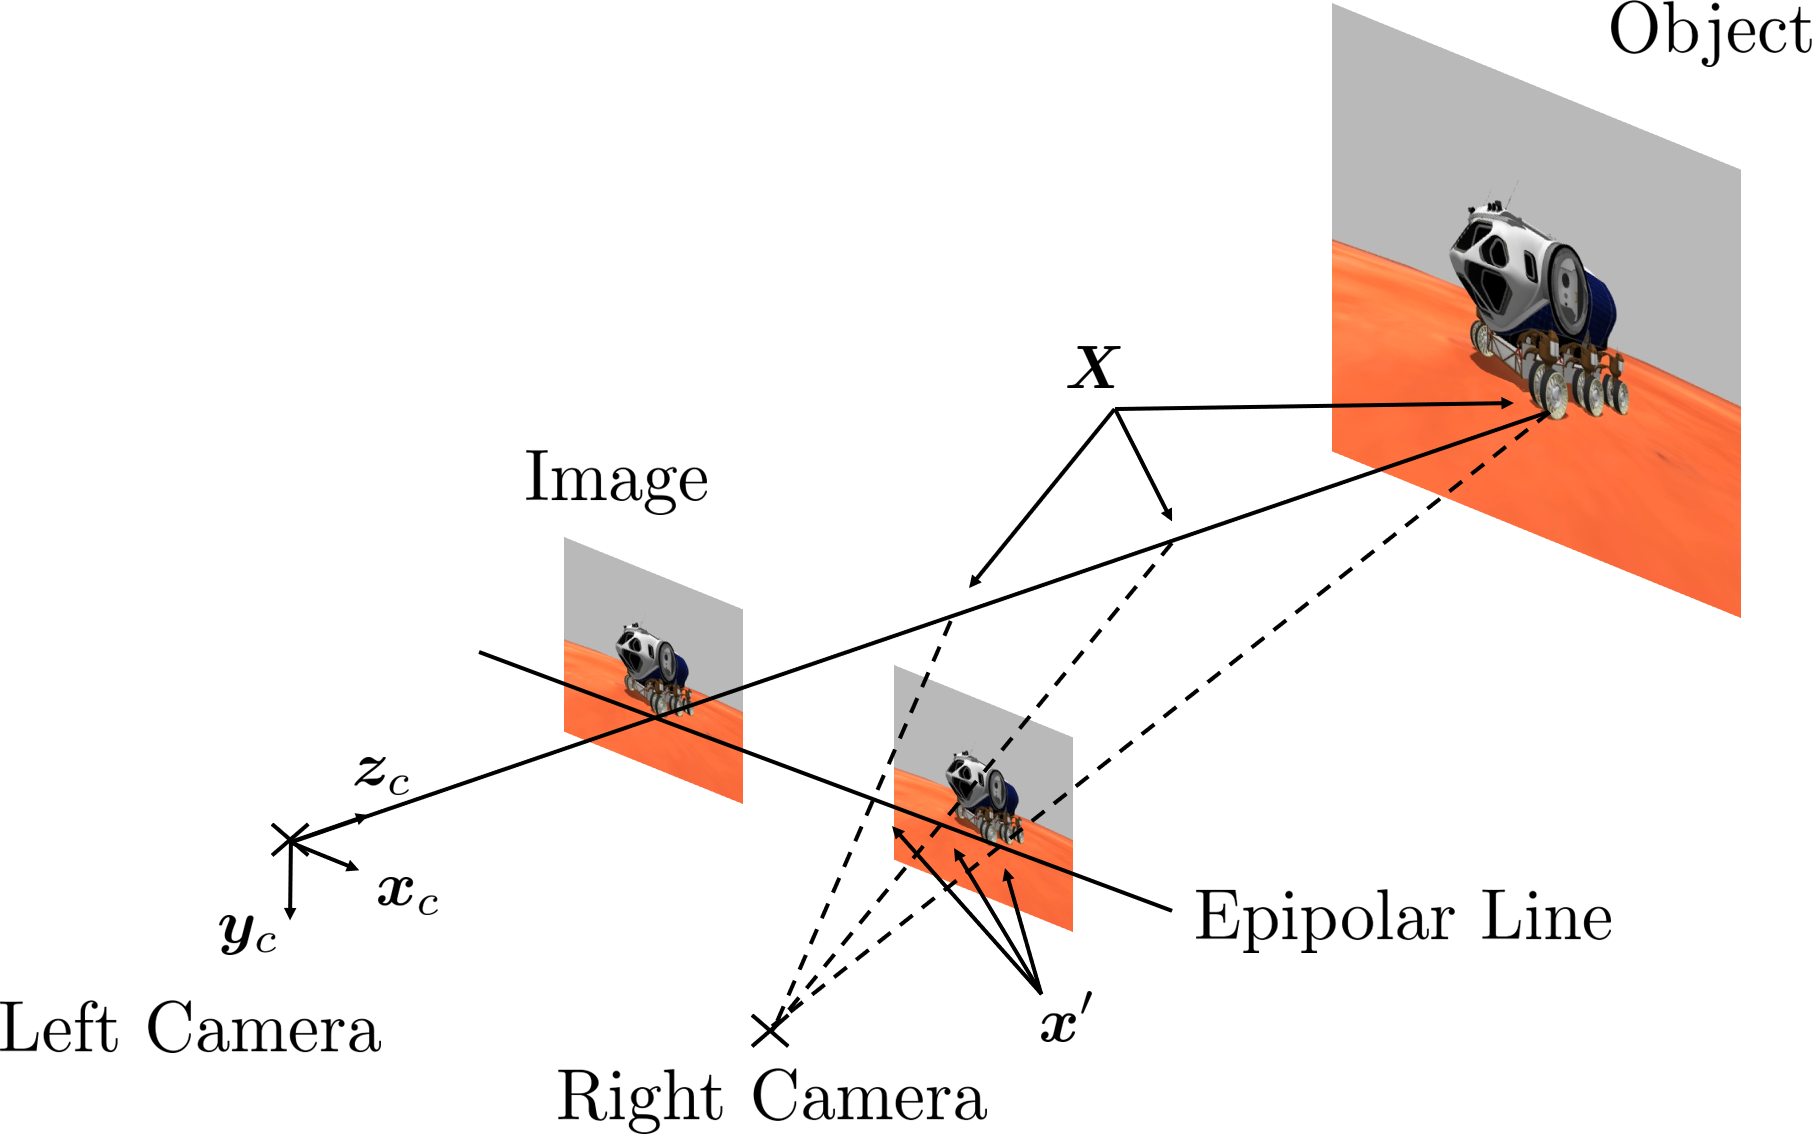
\includegraphics[scale=.28]{chapters/03_background/img/stereo_camera.png}
	\caption{The stereo setup with a left and a right camera.}
	\label{fig::324_stereo_camera}
\end{figure}
It results that, to find correspondences, one only has to search along the epipolar line. Also, since points in the right image that correspond to points in the left image, will always be displaced to the left, one only has to search in this direction. The procedure is shown in figure \ref{fig::324_left_disparity_map}. Instead of looking for single pixel correspondences, it is advised to search for whole block correspondences, since it reduces the noise drastically. Blocks of a defined block size $N$ are taken from the left image, and then the sum of absolute differences SAD is computed for every displacement $d$ in the right image, ranging from zero to number of disparities $D$ (equation \ref{eq::324_sad}, figure \ref{fig::324_left_disparity_map}).
\begin{align}
	\text{SAD}(d) = \sum_{x,y=0}^N |\bm{E}_\text{left}(x,y) - \bm{E}_\text{right}(x-d,y)|
	\label{eq::324_sad}
\end{align}
The disparity $d$ that minimizes the sum of absolute differences SAD is taken to serve as the best correspondence and is therefore used in the disparity map.  Here we can already see that due to the uniqueness of the edge filtered the images $\bm{E}$, it is easier to find correspondences there, rather than in the grayscale or RGB images.
\begin{figure}[h]
	\centering
	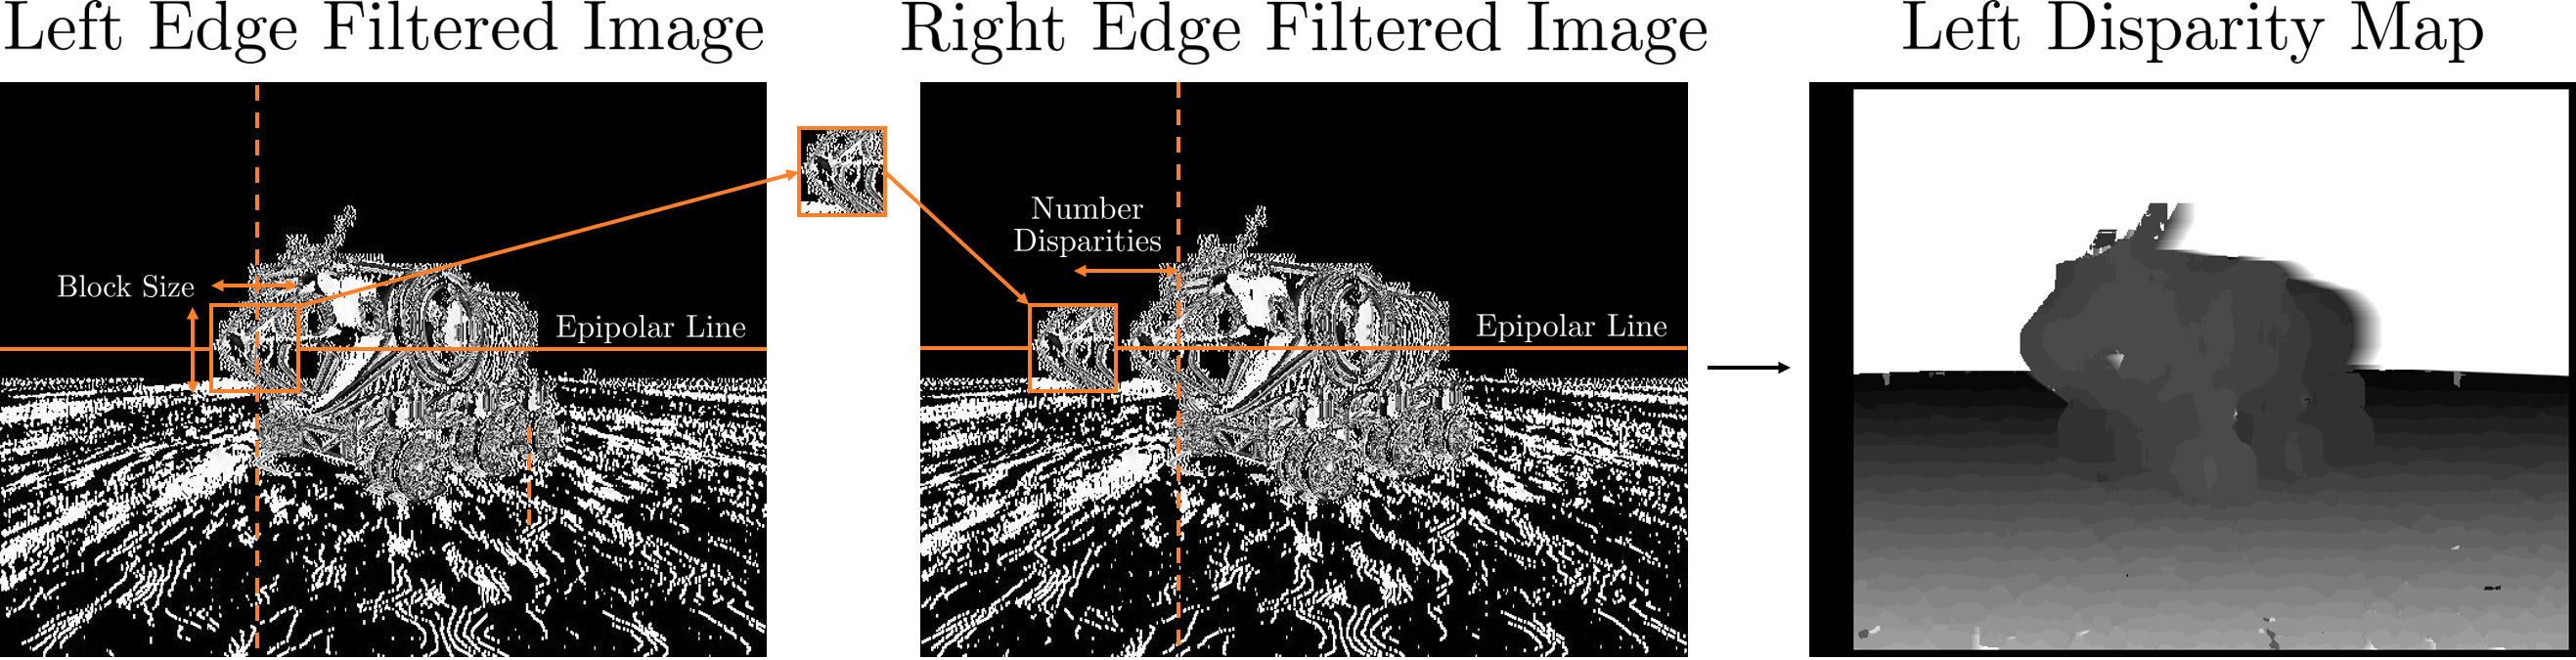
\includegraphics[scale=.28]{chapters/03_background/img/left_disparity_map.png}
	\caption{Generation of the left disparity map by the block matching algorithm.}
	\label{fig::324_left_disparity_map}
\end{figure}
To further refine the disparity map, and especially to assure good results in textureless  regions, we apply a weighted least squares filtering, which is based on the confidence of depth measures. The confidence of depth measures is obtained from the variance within the disparity map $\bm{D}$ (equation \ref{eq::324_variance}, figure \ref{fig::324_confidence_map}).
\begin{align}
	 \text{Var}(\bm{D}) = \mathbb{E}\left[\bm{D}^2\right] - \mathbb{E}\left[\bm{D}\right]^2
	\label{eq::324_variance}
\end{align} 
Therein, the expectation value for $\bm{D}$ is computed by a convolution with the kernel $\bm{K}$ from the following equation
\begin{align}
	\bm{K} &= \alpha
	\begin{pmatrix}
	1 & \dots & 1 \\
	\vdots & \ddots & \vdots \\
	1 & \dots & 1
	\end{pmatrix} \\
	\mathbb{E}\left[\bm{D}\right] &= \bm{K}*\bm{D},
	\label{eq::324_kernel}
\end{align}
where $\alpha = \frac{1}{\text{width}\cdot\text{height}}$ is the normalization factor. The expectation value of the disparity map squared $\mathbb{E}\left[\bm{D}^2\right]$ is computed in the same way, except for that all elements are squared prior to summing them up. Given the variance, we can introduce a concept which is named confidence map. The confidence map $\text{Con}(\bm{D})$ is a measure for the certainty of the computed disparity, and is defined to be linearly dependent on the variance as follows
\begin{align}
	\text{Con}(\bm{D}) = \max\left(1-r\text{Var}(\bm{D}),0\right),
\end{align}
where $r$ is a roll-off factor that defines the change of confidence with growing variance. The resulting disparity confidence is shown in figure \ref{fig::324_confidence_map}, and is used to outweigh outlying disparity values from the final weighted least squares disparity map. 
\begin{figure}[h]
	\centering
	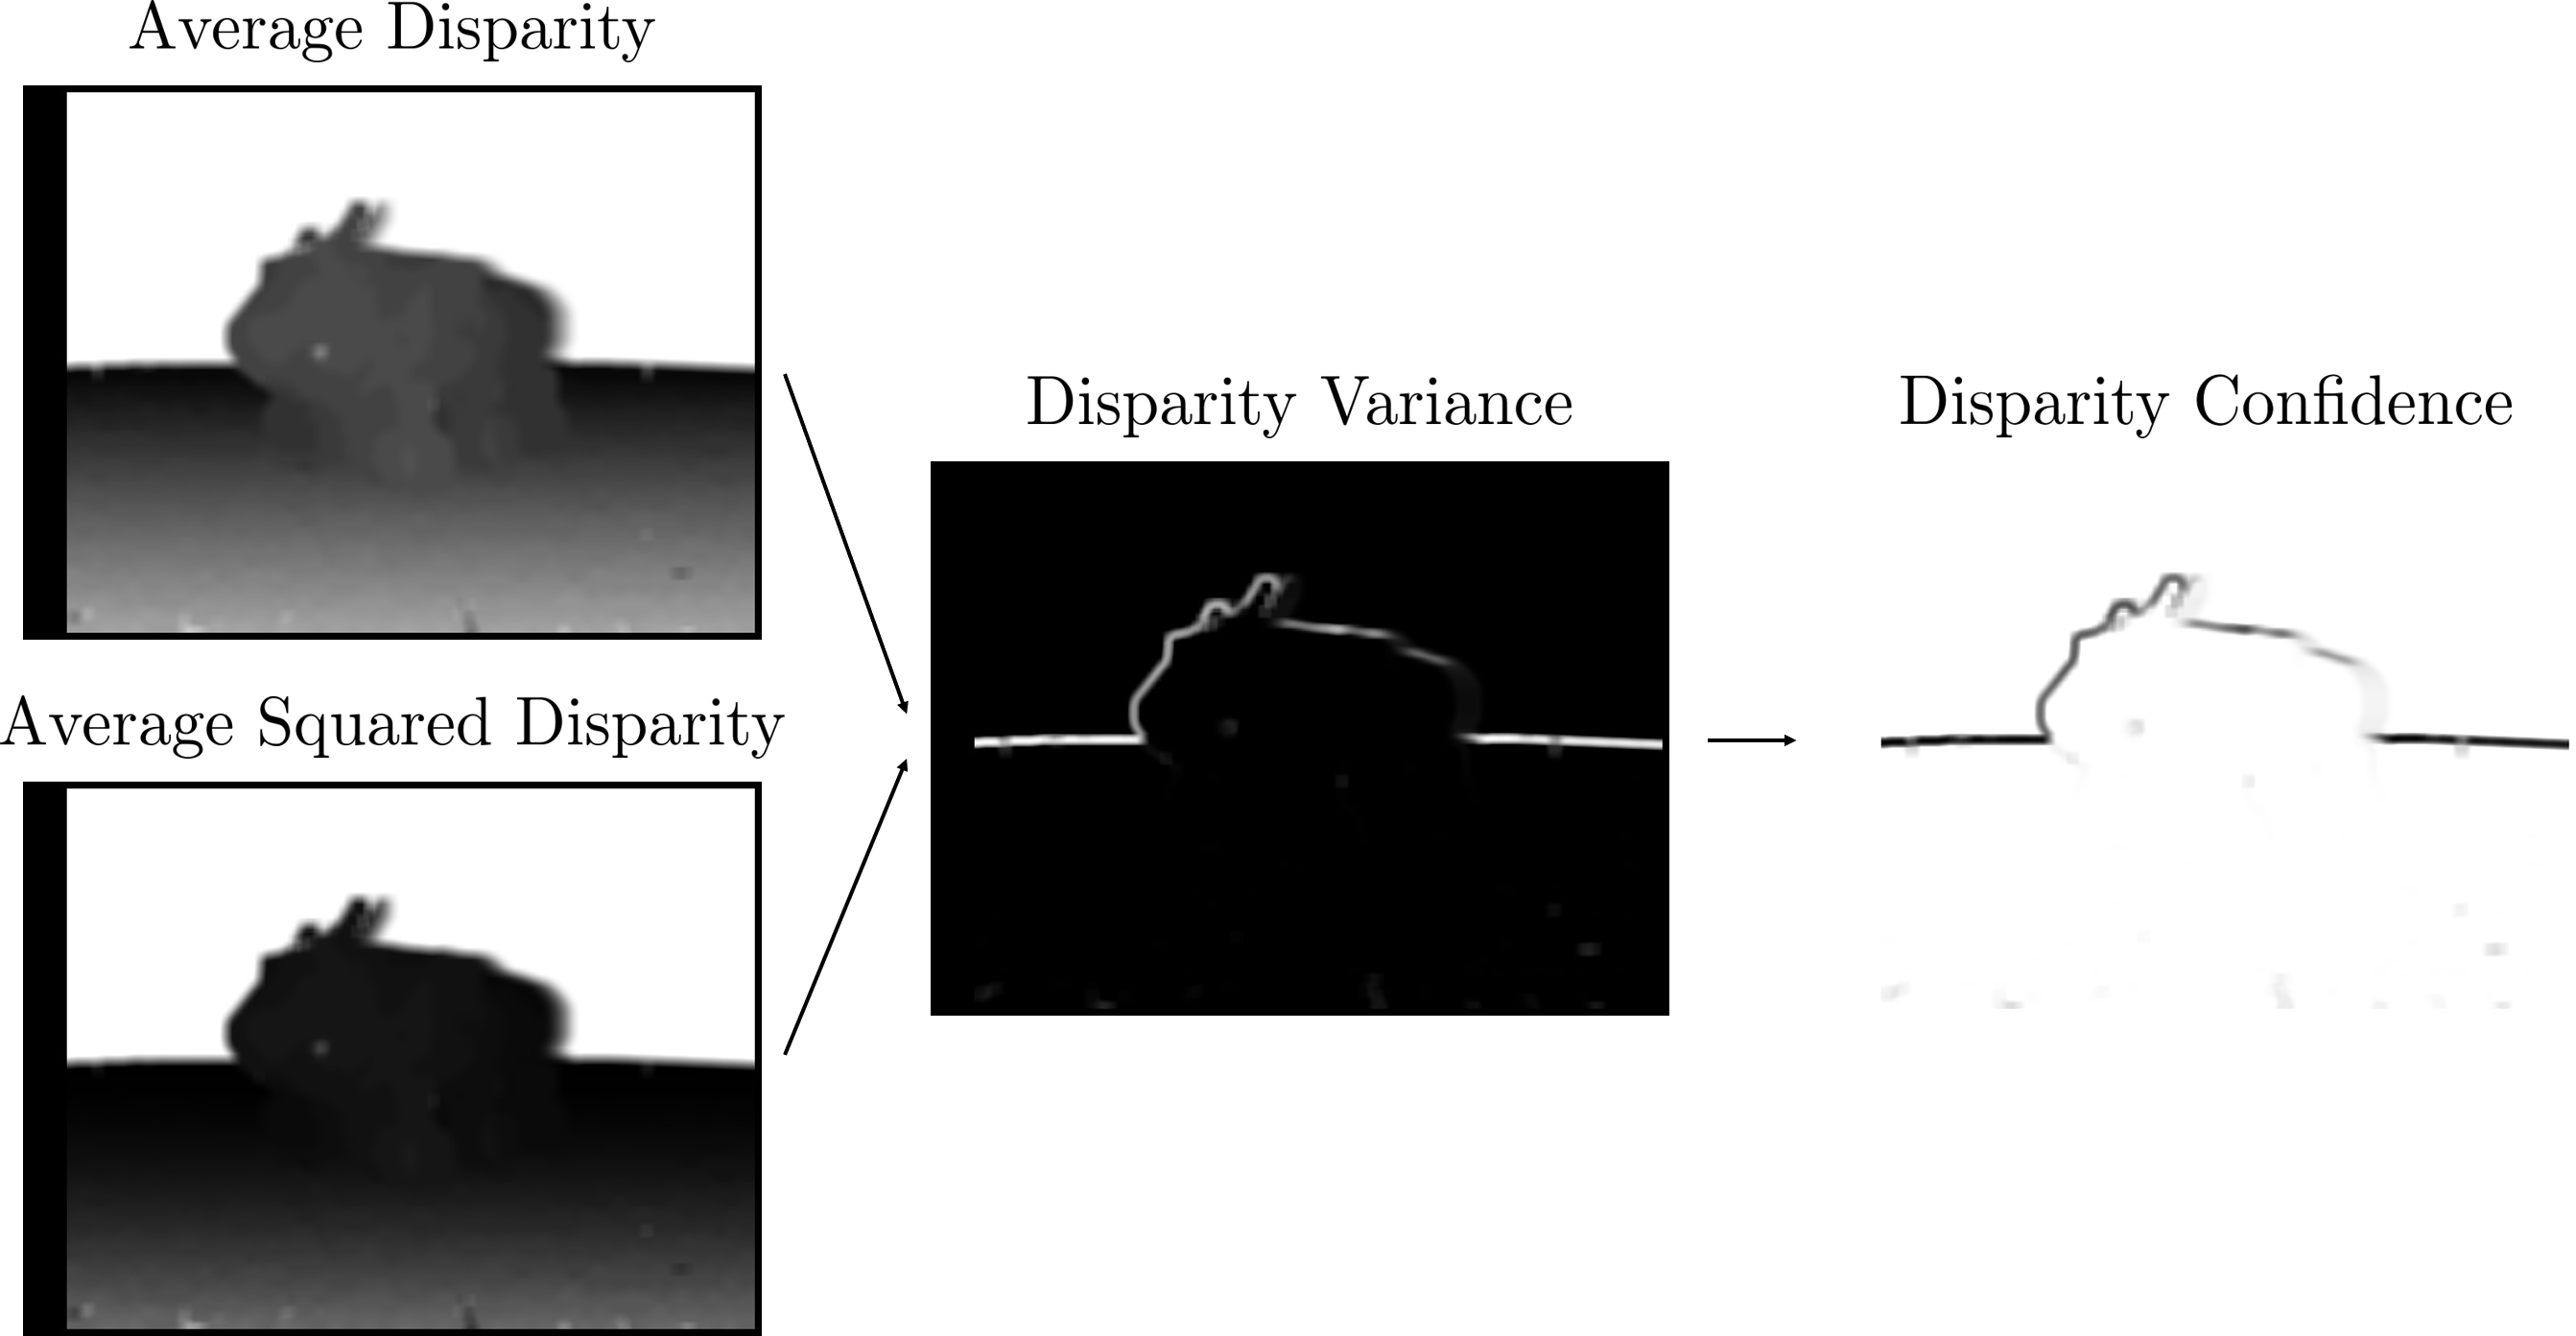
\includegraphics[scale=.28]{chapters/03_background/img/confidence_map.png}
	\caption{Generation of the confidence map from the variance within the disparity map.}
	\label{fig::324_confidence_map}
\end{figure}
Prior to that, we further introduce an additional measure for the prevention of accidentally assigned correspondences in the initial block matching algorithm by using a left right consistency check \cite{egnal2004stereo}. Therefore, the block matching algorithm is used on the right image, and we search for correspondences in the left image. In contrast to the computation of the left disparity map $\bm{D}_\text{left}$, for the right disparity map $\bm{D}_\text{right}$, we only need to check for correspondences along the epipolar line in the positive displacement direction. The left right consistency $\bm{L}$ is then obtained by 
\begin{align}
	\bm{L}(x, y) = 
	\begin{cases}
	\min \left[\text{Con}(\bm{D}_\text{left})(x, y), \text{Con}(\bm{D}_\text{right})(x + d_\text{left}, y)\right] & \text{for } \Delta d < t  \\
	0 & \text{else}
	\end{cases},
\end{align}
where $d_\text{left}$ is the disparity of $\bm{D}_\text{left}$ at position $(x,y)$, and therefore represents the index shift which results from the block matching algorithm. Furthermore, if $\Delta d = \bm{D}_\text{left}(x, y) + \bm{D}_\text{right}(x + d_\text{left}, y)$ is smaller than a threshold $t$, then the left right consistency $\bm{L}$ is taken to be the lower bound approximation of the left and right confidences. Otherwise, the consistency is taken to be false, and hence zero (figure \ref{fig::324_weighted_least_squares_disparity}). As already pointed out, the left right consistency, which is nothing but a confidence measure, usually reveals uncertainties in textureless regions. The weighted least squares filtering that we are about to present uses this fact to its advantage. In a first step, a consistency weighted disparity map $\bm{C}$ is computed via equation \ref{eq::324_cwd} (figure \ref{fig::324_weighted_least_squares_disparity}).
\begin{align}
	\bm{C}=\bm{L}\cdot\bm{D}_\text{left},
	\label{eq::324_cwd}
\end{align}
where $\cdot$ is an element-wise multiplication. Further, the weighted least squares filter is based on the idea of a bilateral filter \cite{tomasi1998bilateral}, and it will try to minimize an energy function $J(\bm{U})$, which takes the original grayscale image as guidance to compute a weight $w_{p,q}$ for neighboring pixels $p$, and $q$ as follows
\begin{align}
	w_{x,y,i,j}(g) = exp(-|g_{x,y}-g_{i,j}|/\sigma).
	\label{eq::324_weight}
\end{align}
Depending on the range parameter $\sigma$, this weight will be high for similar neighboring pixels of the grayscale image $g$, and therefore lead to huge costs in the following energy function $J(\bm{U})$ that we try to minimize
\begin{align}
	J(\bm{U}) = \sum_{x,y}\left[(u_{x,y}-c_{x,y})^2+\lambda\sum_{(i,j)\in\mathcal{N}(x,y)}w_{x,y,i,j}(g)(u_{x,y}-u_{i,j})^2\right],
	\label{eq::324_energy_function}
\end{align}
where $c_{x,y}$ are single pixels of the consistency weighted disparity map. The formulation of this energy function results in a solution $\bm{U}$ that encourages the propagation of disparity values from high- to low-confidence regions (figure \ref{fig::324_weighted_least_squares_disparity}). Additionally, the weight $w$, together with the smoothing parameter $\lambda$, ensure to have similar disparity values in regions with similar texture. The final disparity map $\bm{D}_\text{final}$ is then obtained by normalizing the resulting image $\bm{U}$ with
\begin{align}
	\bm{D}_\text{final} = \frac{\bm{U}}{\text{WLS}(\bm{L})},
	\label{eq::324_wls_final}
\end{align}
where $\text{WLS}(\bm{U})$ is the weighted least squares filtered version of the left right consistency $\bm{L}$.
\begin{figure}[h]
	\centering
	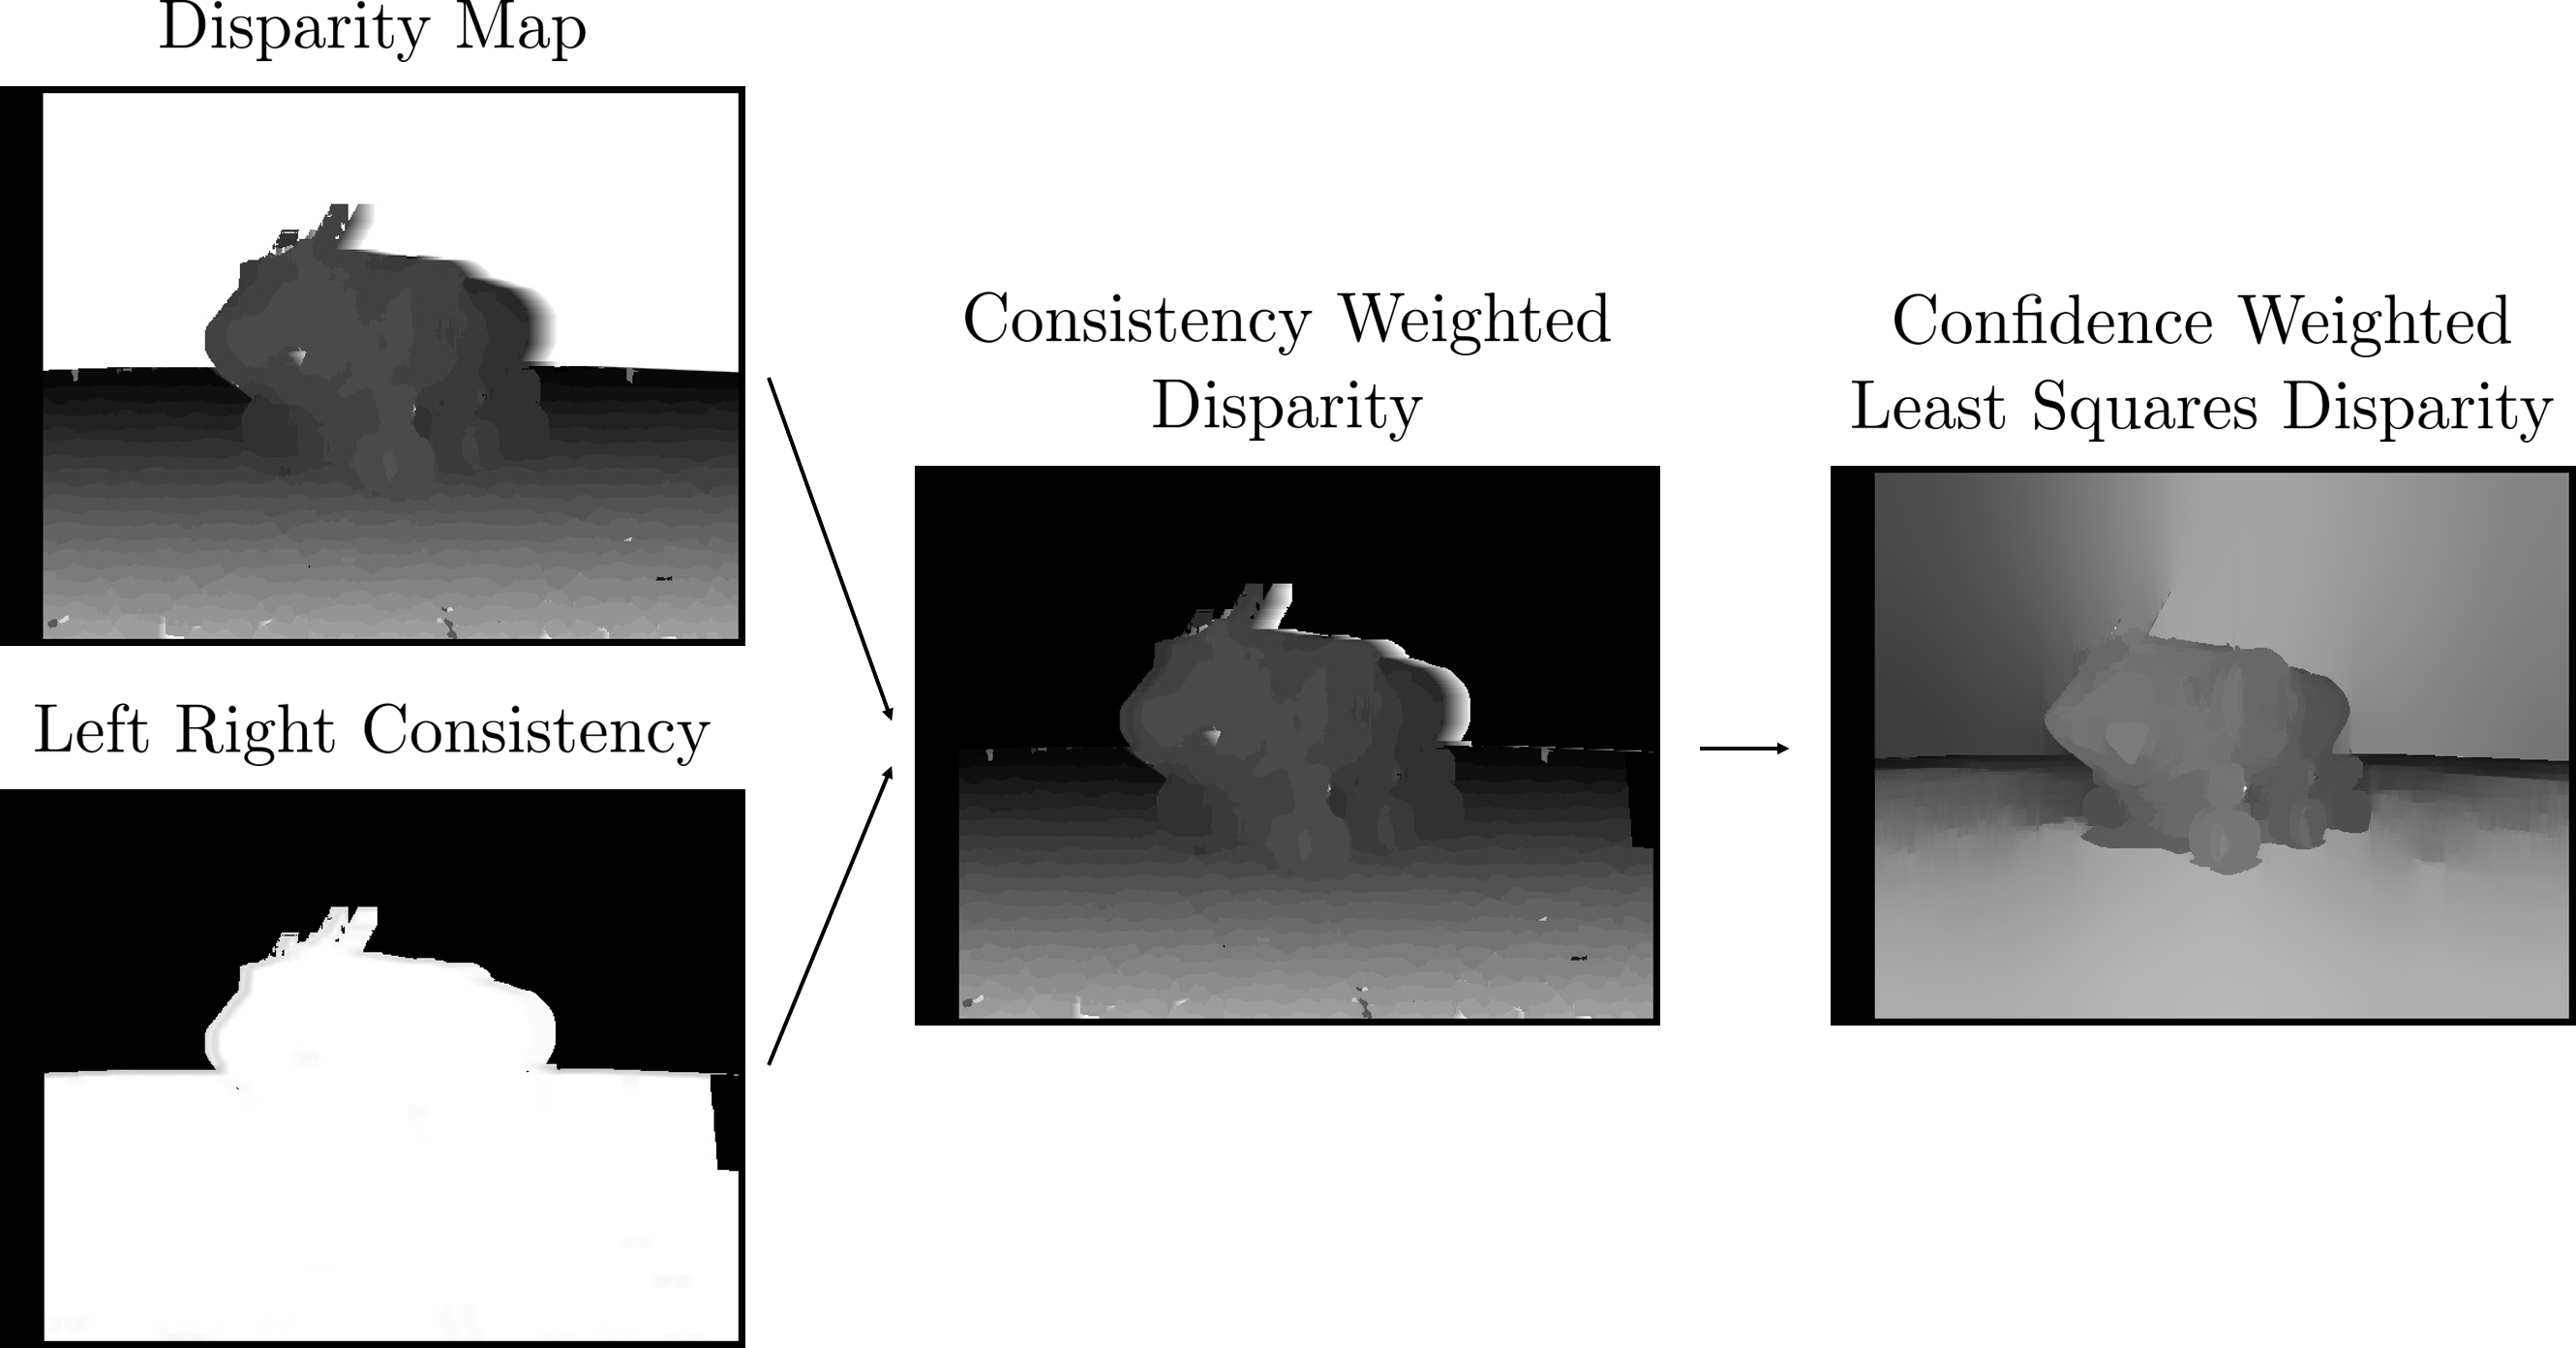
\includegraphics[scale=.28]{chapters/03_background/img/weighted_least_squares_disparity.png}
	\caption{Generation of the confidence weighted least squares disparity from the disparity map, and the left right consistency.}
	\label{fig::324_weighted_least_squares_disparity}
\end{figure}
\\\\
As already mentioned for figure \ref{fig::324_stereo_camera}, the assumption of a simply translated stereo camera pair is almost never correct. In addition, there exist camera intrinsics that deform the observed image, and so the epipolar lines. Therefore, as a requirement for the algorithm to work properly, it is important to calibrate the robot's cameras. The next chapter - Mono and Stereo Camera Calibration, will explain in detail how this is done.
\subsubsection{Mono and Stereo Camera Calibration}
To correct images, as we observe them with a camera, it is required to have a mathematical description of it. A simple one for a camera is the pinhole model, which is shown in figure \ref{fig::324_pin_hole_camera}. For a pinhole camera model, the image plane lies behind the coordinate frame of the camera, and is turned the other way around, but it is easier to describe the image in a virtual plane, which is located at a distance $f$ along the $z_c$-axis, where $f$ is the focal length.
\begin{figure}[h]
	\centering
	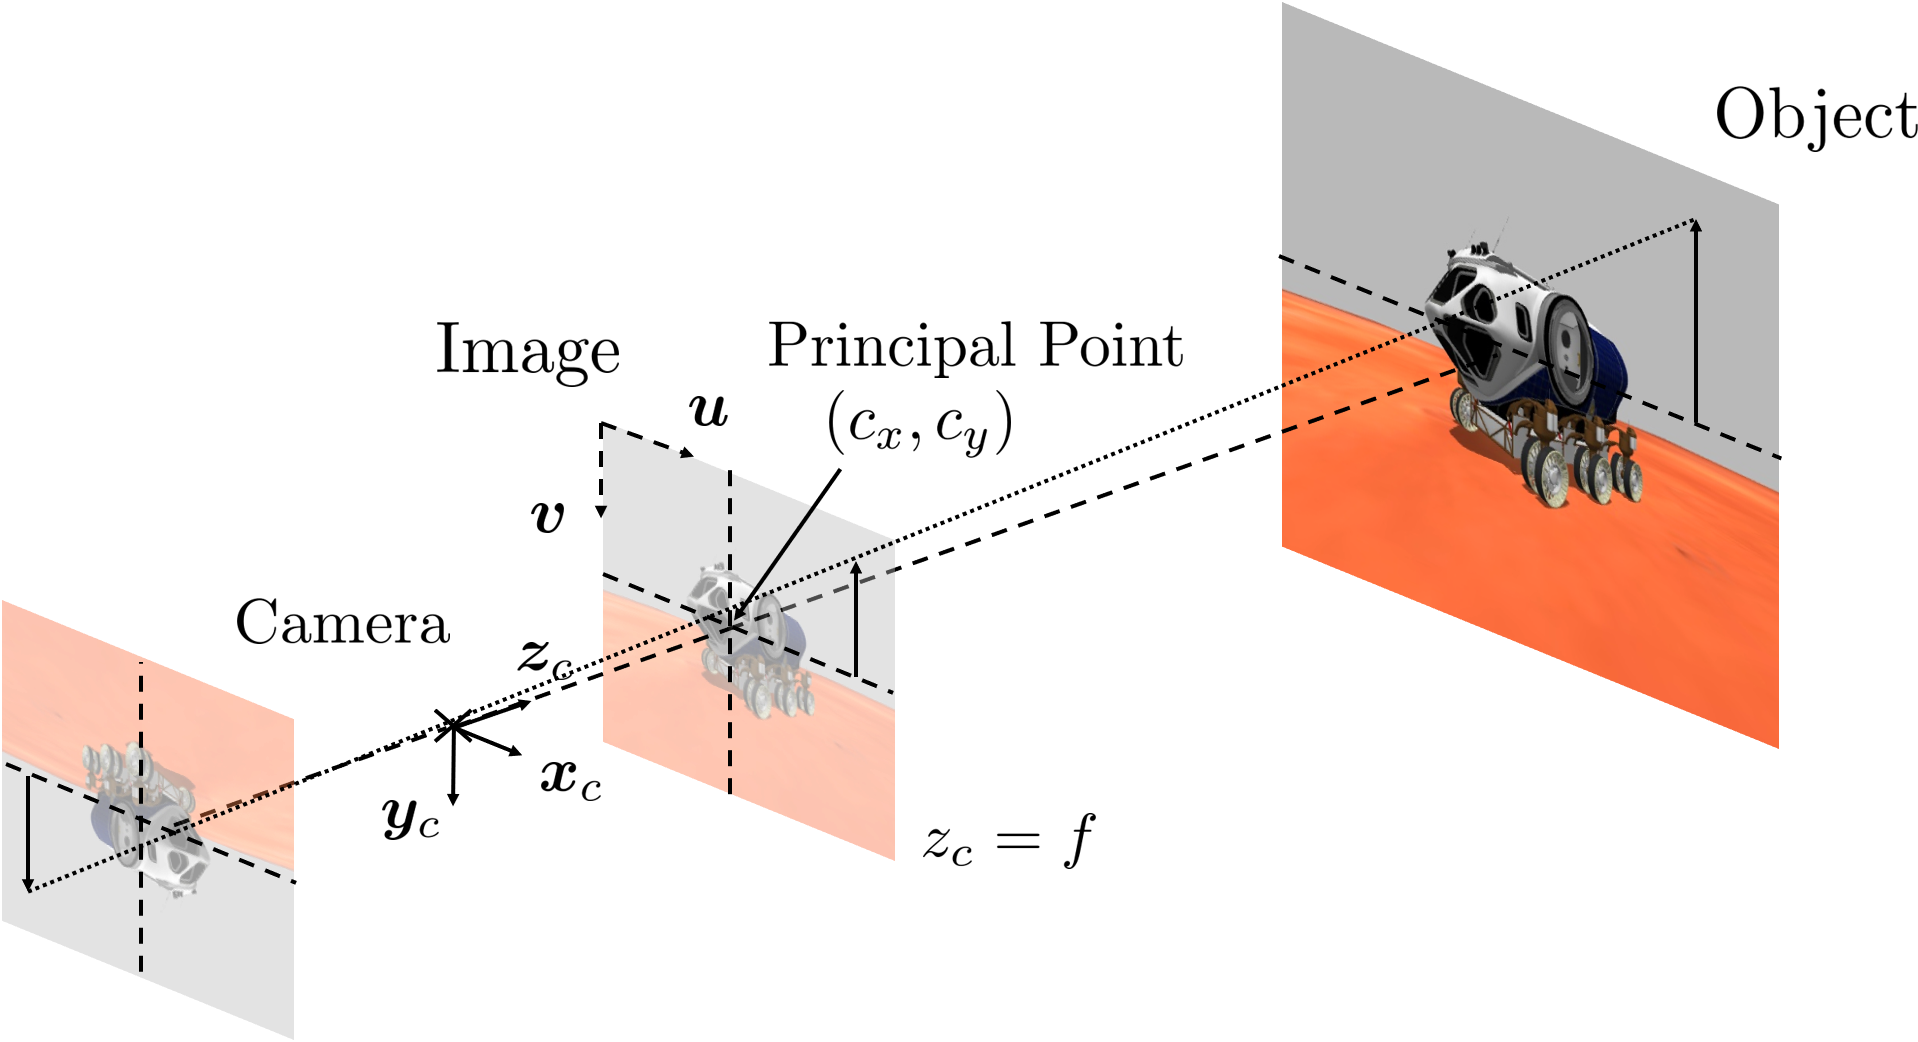
\includegraphics[scale=.28]{chapters/03_background/img/pin_hole_camera.png}
	\caption{Pinhole camera model.}
	\label{fig::324_pin_hole_camera}
\end{figure}
According to the intercept theorem, a point $\bm{X}_c = (X,Y,Z)^T$ is then simply projected to the image plane by the camera matrix $\bm{K}$ with
\begin{align}
	\bm{x}_c = \bm{K}\bm{X}_c = \begin{pmatrix}
	f_x & 0   & c_x \\
	0   & f_y & c_y \\
	0   & 0   & 1
	\end{pmatrix}\bm{X}_c.
	\label{eq::324_focal_intrinsics}
\end{align}
Therein, $\bm{K}$ contains the intrinsic camera parameters, such as the focal lengths and the principal point. For a true pinhole camera $f_x = f_y =f$, but due to errors, usually two different values are chosen. The principal point lies at the position where a light ray connects perpendicularly to the image plane after passing the pinhole, and therefore just defines an offset. For a real setup, it is also required to put a lens at the pinhole's position, which adds some distortion to the image. According to \cite{duane1971close}, we model radial and tangential distortion by
\begin{align}
	x_{c,u} &= x_{c,d}(1+k_1r^2+k_2r^4+k_3r^6) + p_1(r^2+2x_{c,d}^2) + 2p_2x_{c,d}y_{c,d} 
	\label{eq::324_x_dist}\\
	y_{c,u} &= x_{c,d}(1+k_1r^2+k_2r^4+k_3r^6) + 2p_1x_{c,d}y_{c,d} + p_2(r^2+2y_{c,d}^2),
	\label{eq::324_y_dist}
\end{align}
where
\begin{align}
	(x_{c,d}, y_{c,d}) = &\,\,\text{distorted image points within the camera frame $c$,} 
	\nonumber\\
		                 &\,\,\text{as projected onto the image plane}
	\nonumber\\ 
	(x_{c,u}, y_{c,u}) = &\,\,\text{undistorted image points within the camera frame $c$,}
	\nonumber\\
	                     &\,\,\text{as projected by an ideal pinhole camera}
	\nonumber\\
	k_n = &\,\,\text{n$^\text{th}$ radial distortion coefficient}
	\nonumber\\
	p_n = &\,\,\text{n$^\text{th}$ tangential distortion coefficient}
	\nonumber\\
	r = &\,\,\sqrt{x_{c,d}^2+y_{c,d}^2}.
	\nonumber
\end{align}
Together, the focal lengths, the principal point, and the distortion coefficients make up the unknowns within our camera model. Goal of the mono camera calibration is now to find these coefficients from images of a well known calibration pattern. Therefore, images of the calibration pattern are taken from different perspectives (figure \ref{fig::324_calibration_process}). 
\begin{figure}[h]
	\centering
	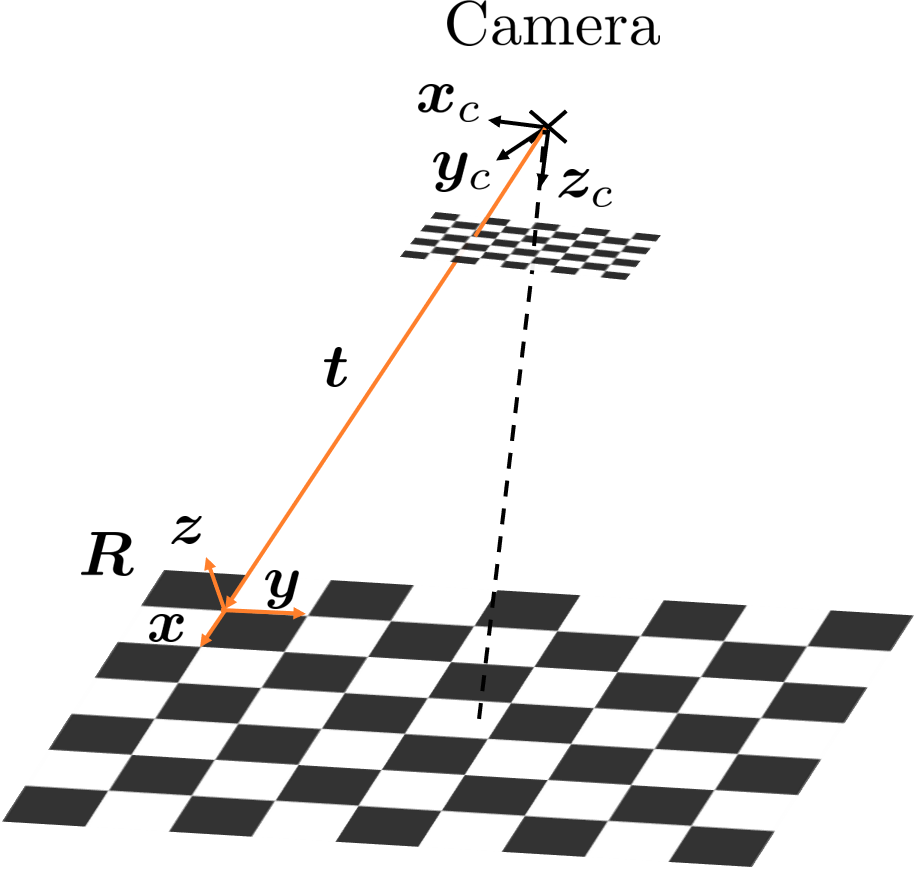
\includegraphics[scale=.28]{chapters/03_background/img/calibration_process.png}
	\caption{Calibration pattern as observed from the camera's coordinate system $C$. Within the object's coordinate system, all chessboard corners lie at a zero $z$-position.}
	\label{fig::324_calibration_process}
\end{figure}
For the mathematical description, the calibration pattern is taken to be at a fixed position and orientation, while it is assumed that the camera was moved. The position of each corner can then be described by the square's size $a$ as follows
\begin{align}
	\bm{x}_{nm} = \begin{pmatrix}
	wa & ha & 0 & 1
	\end{pmatrix}^T,
	\label{eq::324_square_size}
\end{align}
where we now switched to homogeneous coordinates, and $w\in[0,W],h\in[0,H]$ are whole numbers, corresponding to the width and the height of the pattern. It is then required to find the rotation $\bm{R}$ and translation $\bm{t}$, which transforms the object points to the image plane. They are estimated by solving a perspective-n-point problem \cite{fischler1981random}. Therefore, as shown in figure \ref{fig::324_distortion} (b), a corner detecting algorithm finds the corners $\bm{x}_{c,wh}$ within the image plane. Under the assumption of known intrinsic camera parameters, $\bm{x}_{c,wh}$ are then being undistorted according to equations \ref{eq::324_x_dist} and \ref{eq::324_y_dist}. 
\begin{figure}[h]
	\centering
	\subcaptionbox{}%
	[.4\linewidth]{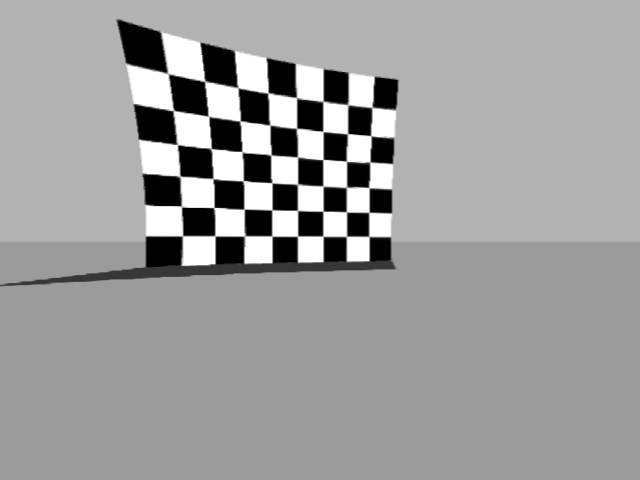
\includegraphics[scale=.2]{chapters/03_background/img/gazebo_calib_left.jpg}}
	\subcaptionbox{}%
	[.4\linewidth]{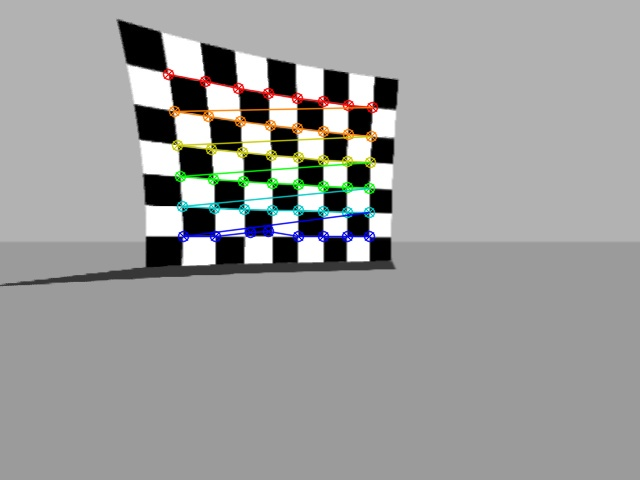
\includegraphics[scale=.2]{chapters/03_background/img/gazebo_corners.jpg}}
	\caption{Distorted calibration pattern (a), and the image points as found by the algorithm (b).}
	\label{fig::324_distortion}
\end{figure} 
Each $\bm{x}_{nm}$ can then be transformed to the camera's frame, and further be projected onto the image plane via
\begin{align}
	\bm{x}_{c,wh} = \bm{K}\begin{pmatrix}
	\bm{R} & \bm{t}
	\end{pmatrix}\bm{x}_{wh},
\end{align}
where $\bm{R}$ describes the rotation, and $\bm{t}$ the translation of the camera frame to the object frame. Then, equations \ref{eq::324_x_dist} and \ref{eq::324_y_dist} are applied to obtain the undistorted image points from $\bm{x}_{c,wh}$. The undistorted image points $\bm{x}_{c,wh,u}$ are then being reprojected by inverting the rotation and translation via
\begin{align}
	\bm{x}_{wh,u} = \begin{pmatrix}
	\bm{R} & \bm{t}
	\end{pmatrix}^{-1}\bm{x}_{c,wh,u},
	\label{eq::324_reprojection}
\end{align}
from which we compute the re-projection error $\Delta x = ||\bm{x}_{wh,u} - \bm{x}_{wh}||_2$. To find the intrinsic parameters, a Levenberg-Marquardt algorithm then optimizes them in an iterative scheme to minimize the re-projection error until convergence \cite{zhang2000flexible}. The stereo camera calibration can then be performed by applying the mono camera calibration to each camera separately, from which the camera intrinsics are obtained. Given the camera intrinsics of both cameras, it is again possible to solve a perspective-n-point problem, which yields the positions and orientations of both cameras with respect to the observed object. This enables us to compute the fundamental matrix $\bm{F}$, which transforms points from the left camera's view $\bm{x}_{c_\text{left}}$, to points $\bm{x}_{c_\text{right}}$, as seen by the right camera via
\begin{align}
	\bm{x}_{c_\text{right}}^T\bm{F}\bm{x}_{c_\text{left}} = \bm{0}
\end{align}
The mapping enables us to rectify the left and the right image \cite{loop1999computing}, using the rectification transforms $\bm{R}_i$, which means that we can compute homography transforms that align epipolar lines within the images (figure \ref{fig::324_rectified}), which where previously defined by the fundamental matrix. 
\begin{figure}[h]
	\centering
	\subcaptionbox{}%
	[.4\linewidth]{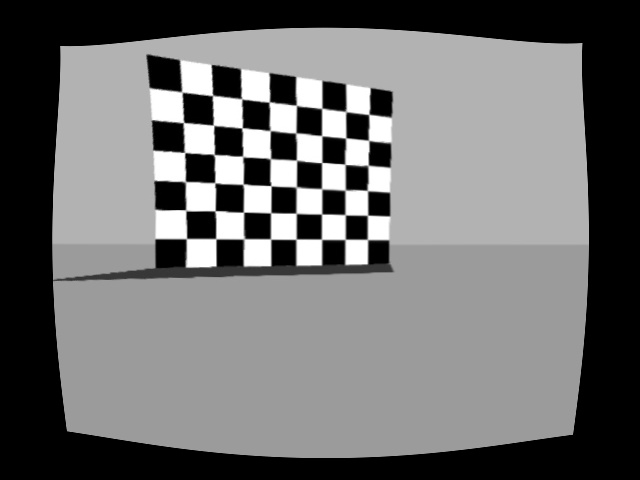
\includegraphics[scale=.2]{chapters/03_background/img/gazebo_rectified_left.jpg}}
	\subcaptionbox{}%
	[.4\linewidth]{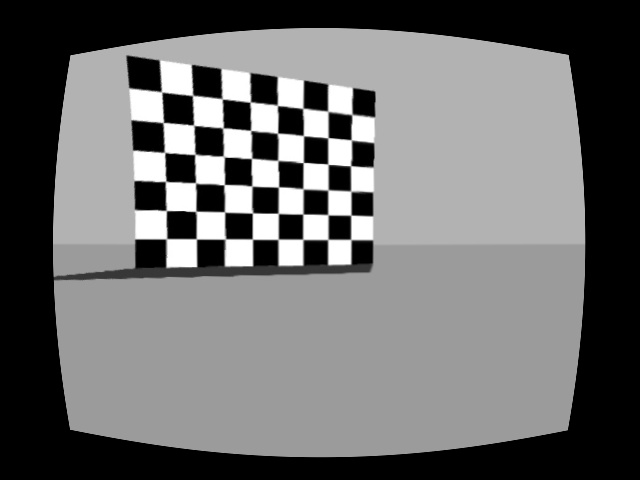
\includegraphics[scale=.2]{chapters/03_background/img/gazebo_rectified_right.jpg}}
	\caption{Undistorted calibration pattern, as observed by the left camera (a), and by the right camera (b). For comparison, see the distorted calibration pattern in figure \ref{fig::324_distortion}, and note how the horizons within the images align.}
	\label{fig::324_rectified}
\end{figure}
These homography transforms map the images, as we observe them with the cameras, to a shared virtual plane, which is defined by the newly obtained projection matrices $\bm{P}_i$. Therefore, we reached our initial goal, since it enables us to apply the stereo block matching algorithm, which got introduced earlier, to the transformed images.   % image processing
   
  \chapter{Methods}
  \section{Software}
  %\input{chapters/04_methods/01_eig}     % eigen
  %\input{chapters/04_methods/02_qp}      % qpoases
  %\input{chapters/04_methods/03_rbdl}    % rbdl
  %\input{chapters/04_methods/04_yarp}    % yarp
  %\input{chapters/04_methods/05_pyt}     % pytorch
  %\input{chapters/04_methods/06_cv}      % opencv
  
  \section{Implementation}  
   
  \chapter{Experiments}
  Within the experiments chapter, we will first benchmark the nonlinear model predictive control implementation of ours for purely simulated tasks in section \ref{sec::51_uc}, and then tune hyperparameters for it to run well on Heicub. This will allow us to define a standardized environment for walking experiments in section \ref{sec::512_pt}, to later compare user controlled performance against autonomously controlled performance in section \ref{sec::52_aw}. Though, before we can tackle the idea of behavioral cloning, which got described in section \ref{sec::322_bc}, we need to meat the prerequisites, that is we will calibrate the camera, and tune the depth map parameter extraction in sections \ref{sec::521_cc}, and \ref{sec::522_dp}, respectively. All of the above mentioned steps, will then allow us to collect data and to train a newly developed neural network architecture on it in section \ref{sec::523_da}. Finally, we will compare the humanly controlled robot's balance with the artificially controlled robot's balance in section \ref{sec::524_pt}, and investigate on the reinforcement learning approach for autonomous navigation in section \ref{sec::525_pp}.
  \section{Camera Calibration}
\label{sec::51_cc}
As described in section \ref{sec::324_ip}, in order for the stereo block matching algorithm to work properly (equation \ref{eq::324_sad}), it is required to calibrate the cameras. We therefore chose to use a chess-board calibration pattern, see figure \ref{fig::51_calib}. The used calibration pattern has width of $W=8$, and a height of $H=6$, where each square has a size of $a=22.5\,\text{mm}$ (equation \ref{eq::324_square_size}). We took a total of $N=60$ images of the calibration pattern for varying orientations and translations with respect to the camera, which results in a total of $W\times H\times N = 2880$ points for the calibration. 
\begin{figure}[h]
	\centering
	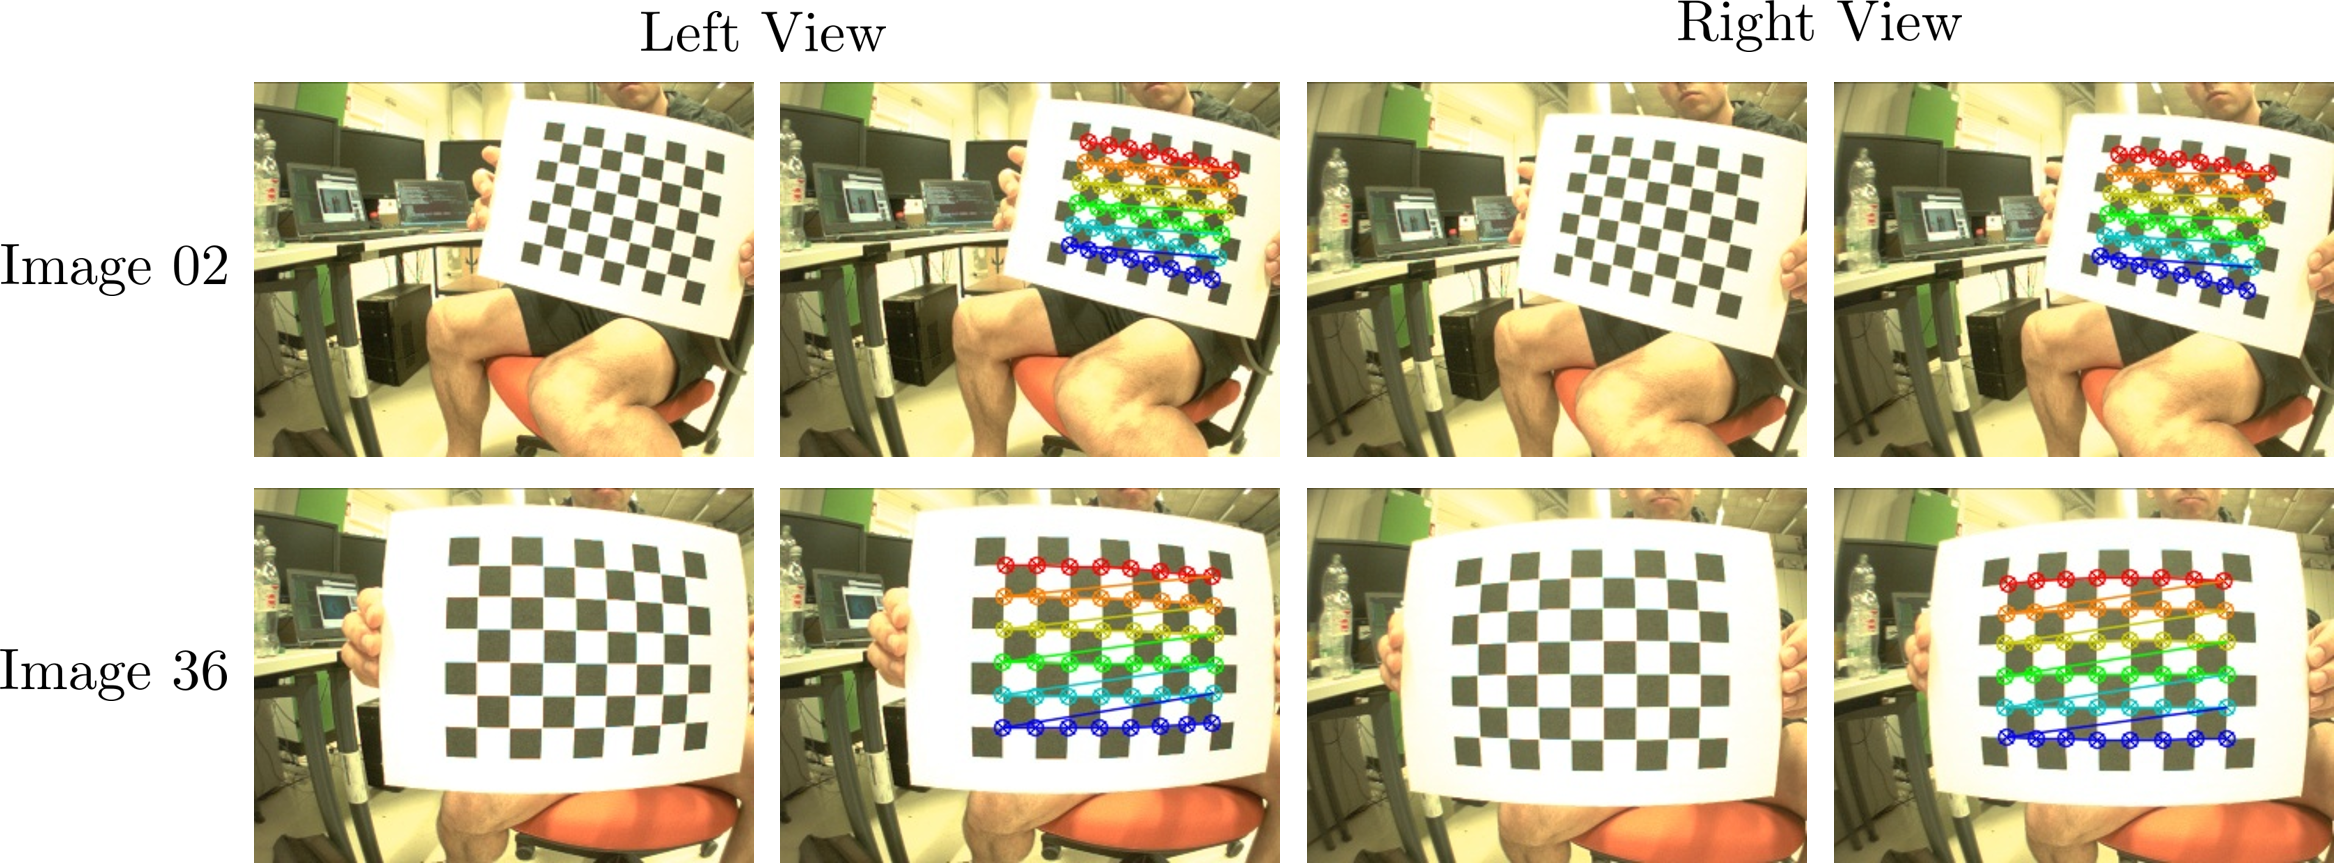
\includegraphics[scale=.28]{chapters/05_experiments/01_camera_calibration/calib.png}
	\caption{Exemplary left and right camera views of the calibration pattern as acquired during the calibration process. The colorful points indicate the detected corners in the image plane. Refer to figure \ref{fig::324_distortion} for the theory.}
	\label{fig::51_calib}
\end{figure}
oAs the resulting mean squared re-projection error $\Delta \bar{x} = 1/(WHN)\sum_0^{WHN} \Delta x$ (equation \ref{eq::324_reprojection}), we obtained $\Delta \bar{x}_l = 0.26\, \text{pixel}$, and $\Delta \bar{x}_r = 0.25\,\text{pixel}$, for the left, and the right camera, respectively. According to equations \ref{eq::324_focal_intrinsics}, \ref{eq::324_x_dist}, and \ref{eq::324_y_dist}, we therefore determined the camera intrinsic parameters as listed in table \ref{tab::51_intrinsics}.
\begin{table}
	\centering
	\begin{tabular}{lll}
		Intrinsic Parameter & Left Camera & Right Camera\\
		\hline
		$f_x$ & $\quad2.36\cdot10^2$ & $\quad2.32\cdot10^2$ \\
		$f_y$ & $\quad2.37\cdot10^2$ & $\quad2.32\cdot10^2$ \\
		$c_x$ & $\quad1.63\cdot10^2$ & $\quad1.86\cdot10^2$ \\
		$c_y$ & $\quad1.11\cdot10^2$ & $\quad1.30\cdot10^2$ \\
		$k_1$ & $-4.54\cdot10^{-1}$ & $-4.58\cdot10^{-1}$ \\
		$k_2$ & $\quad2.90\cdot10^{-1}$  & $\quad3.18\cdot10^{-1}$  \\
		$k_3$ & $-1.21\cdot10^{-1}$ & $-1.48\cdot10^{-1}$ \\
		$p_1$ & $-2.73\cdot10^{-3}$ & $\quad3.02\cdot10^{-4}$  \\
		$p_2$ & $\quad2.16\cdot10^{-4}$  & $\quad7.63\cdot10^{-4}$		
	\end{tabular}
	\caption{Intrinsic parameters of single cameras. These parameters can be found as YAML file on GitHub (\href{https://github.com/mhubii/nmpc_pattern_generator/tree/master/libs/io_module}{link}).\label{tab::51_intrinsics}}
\end{table}
Then given the calibration of each single camera, we computed the rectification transforms $\bm{R}$, and the projection matrices $\bm{P}$ in the rectified coordinate system for each camera \ref{tab::51_extrinsics}.
\begin{table}
	\centering
	\begin{tabular}{lll}
		Camera & Extrinsic Parameter & \\ 
		\hline
		&& \\
		\multirow{5}{*}{Left} & $\bm{R}$              & $\begin{pmatrix}
		\quad9.93\cdot10^{-1} & -2.65\cdot10^{-3}     & \quad1.14\cdot10^{-1} \\ 
		\quad5.41\cdot10^{-1} & \quad1.00\cdot10^{0}  & -2.39\cdot10^{-2} \\
		-1.14\cdot10^{-1}     & \quad2.43\cdot10^{-2} & \quad9.93\cdot10^{-1}
		\end{pmatrix}$ \\&&\\
		                      & $\bm{P}$              & $\begin{pmatrix}
        2.34\cdot10^{2} & 0.00     & 1.88\cdot10^{2} & 0.00 \\ 
        0.00 & 2.34\cdot10^{2}  & 4.87\cdot10^{1} & 0.00 \\
        0.00    & 0.00 & 1.00 & 0.00
        \end{pmatrix}$ \\
        &&\\
        \multirow{5}{*}{Right} & $\bm{R}$              & $\begin{pmatrix}
        \quad9.95\cdot10^{-1} & -2.30\cdot10^{-2}     & \quad9.93\cdot10^{-2} \\ 
        \quad2.07\cdot10^{-2} & \quad1.00\cdot10^{0}  & \quad2.38\cdot10^{-2} \\
        -9.98\cdot10^{-2}     & -2.16\cdot10^{-2} & \quad9.95\cdot10^{-1}
        \end{pmatrix}$ \\&&\\
        & $\bm{P}$              & $\begin{pmatrix}
        2.34\cdot10^{2} & 0.00     & 1.88\cdot10^{2} & -1.60\cdot10^1 \\ 
        0.00 & 2.34\cdot10^{2}  & 4.88\cdot10^{1} & 0.00 \\
        0.00    & 0.00 & 1.00 & 0.00
        \end{pmatrix}$ \\
	\end{tabular}
	\caption{Rectification transform $\bm{R}$, and projection matrices $\bm{P}$, for the left, and the right camera, respectively. These parameters can be found as YAML file on GitHub (\href{https://github.com/mhubii/nmpc_pattern_generator/blob/master/libs/io_module/cam_stereo.yaml}{link}). \label{tab::51_extrinsics}}
\end{table}
Exemplary rectified images, which rely on the matrices of table \ref{tab::51_extrinsics}, are shown in figure \ref{fig::51_rect}. Since there is a slight rotation of the calibration pattern, it is not obvious that the images got rectified well. Therefore, the same images are shown in figure \ref{fig::51_rect_line}, but slightly rotated such that the calibration pattern aligns horizontally. The blue line therein indicates that in contrast to the original image, straight lines now appear straight across both images, which is crucial for the block matching algorithm in the next section - Depth Map Parameter Tuning.
\begin{figure}[h]
	\centering
	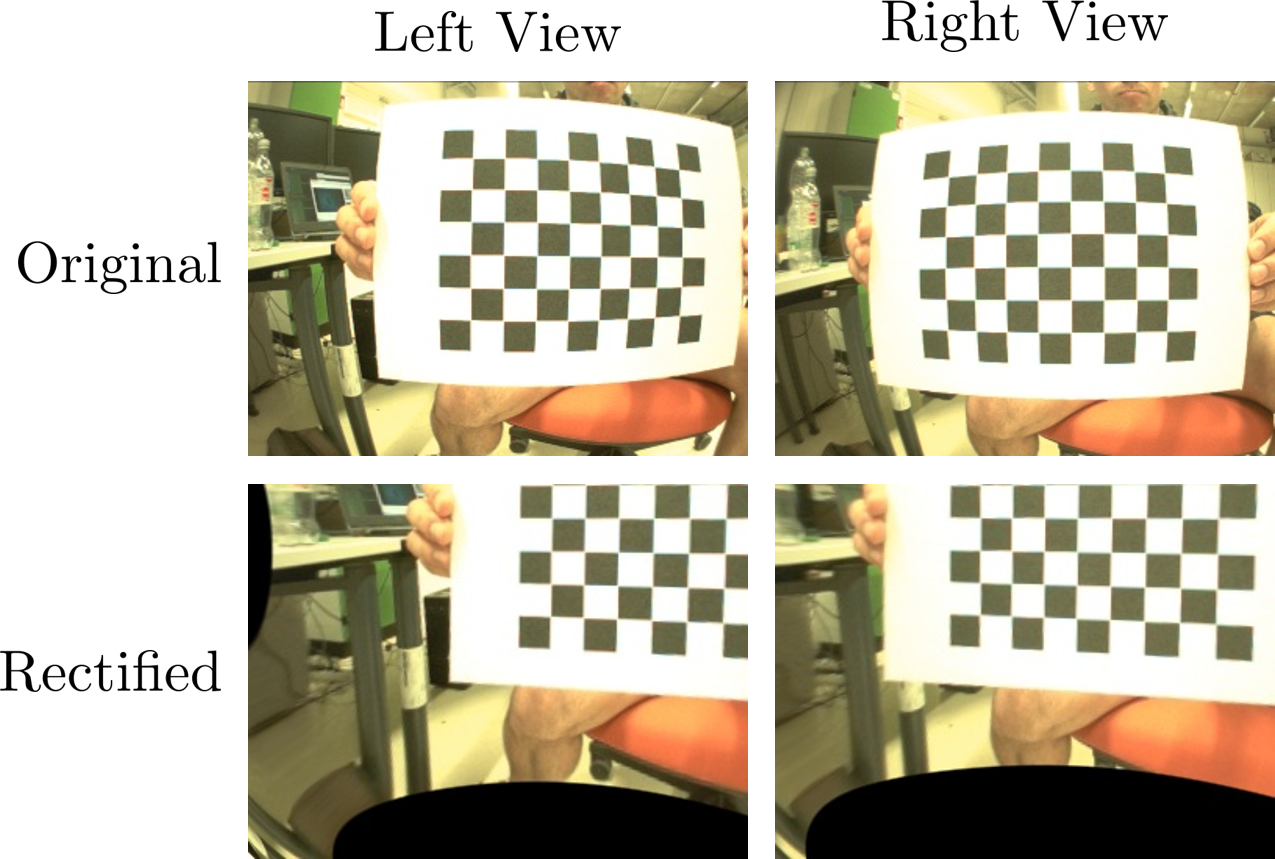
\includegraphics[scale=.28]{chapters/05_experiments/01_camera_calibration/rect.png}
	\caption{Rectified and original view of the stereo camera. Due to a slight rotation of the calibration pattern, it does not immediately become clear that the image got rectified correctly, see figure \ref{fig::51_rect_line}. Refer to figure \ref{fig::324_rectified} for the theory.}
	\label{fig::51_rect}
\end{figure}
\begin{figure}[h]
	\centering
	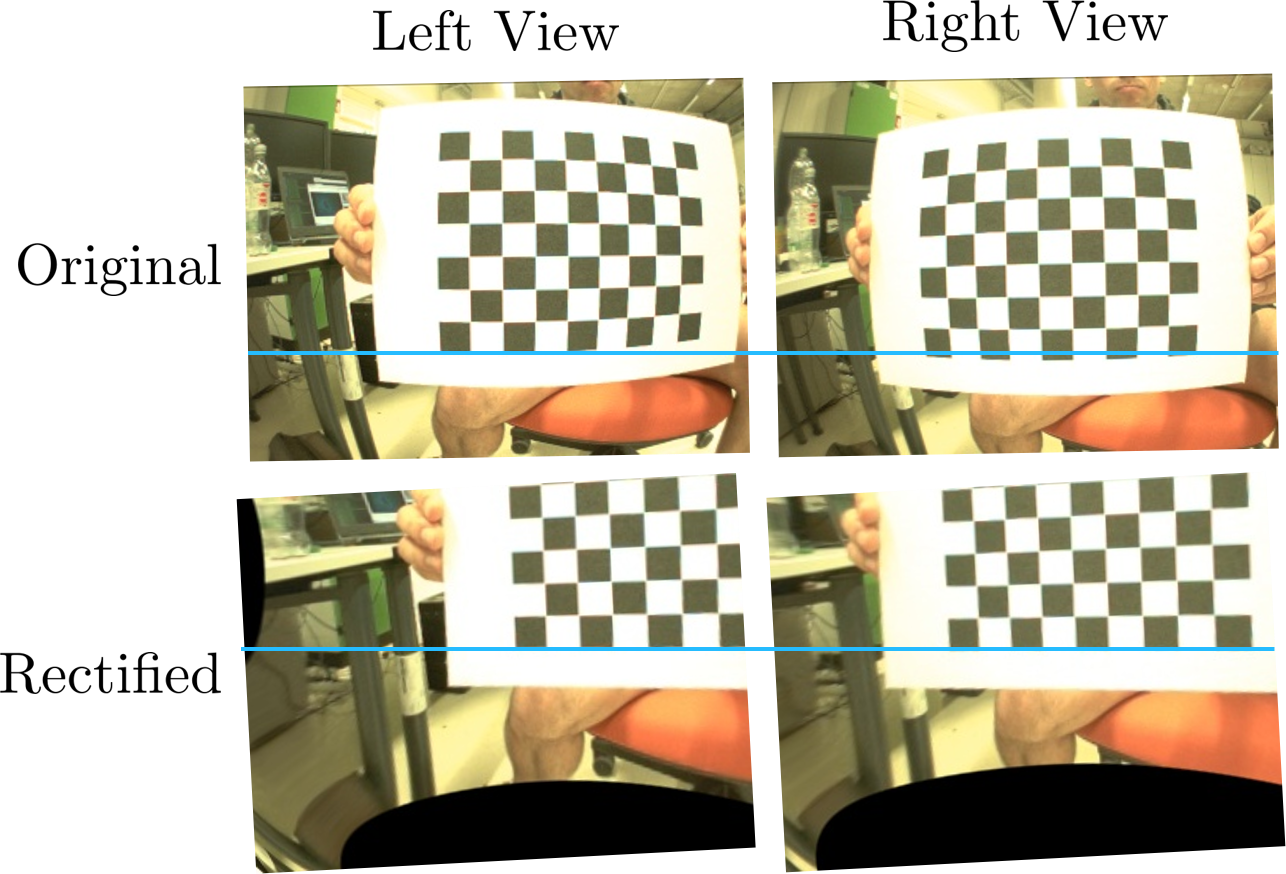
\includegraphics[scale=.28]{chapters/05_experiments/01_camera_calibration/rect_line.png}
	\caption{Same images as shown in figure \ref{fig::51_rect}, but rotated such that the blue line indicates that straight lines are now indeed straight. Please note that the blue lines do not correspond to the epipolar lines, but to rotated versions of them.}
	\label{fig::51_rect_line}
\end{figure}

  \section{Depth Map Parameter Tuning}
\label{sec::52_dm}
Within this section, we shortly explore the effects of all tunable parameters on the depth map generation. Therefore, we utilize a simple experimental setup, which is shown in figure \ref{fig::52_wls_setup}.
\begin{figure}[h]
	\centering
	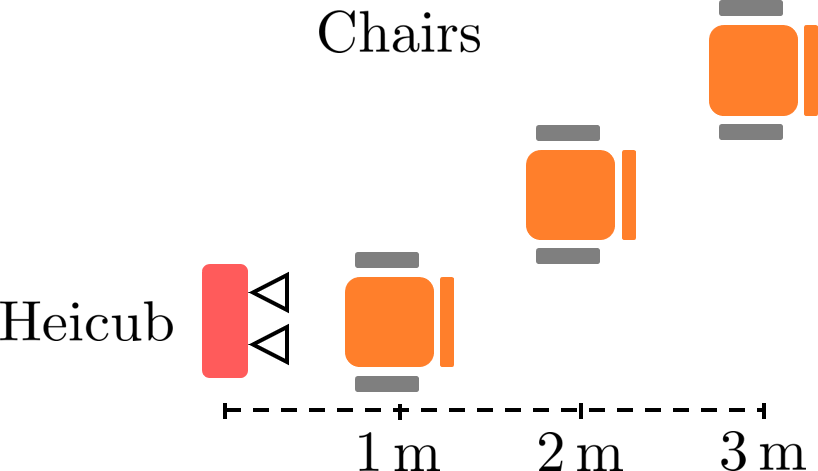
\includegraphics[scale=.4]{chapters/05_experiments/02_depth_map_parameter_tuning/wls_setup.png}
	\caption{Setup for the parameter tuning of the depth map extraction. Heicub's cameras are indicated by the two triangles, of which you can find the view in figure \ref{fig::52_wls_rgb}}
	\label{fig::52_wls_setup}
\end{figure}
Within the setup, Heicub points its stereo camera towards three chairs that are located at a distance of $1\,\text{m}$ towards each other, and towards the cameras, so to cover close, medium, and far distances. The consecutive chairs are slightly shifted, in order to enable the simultaneous observation of all of them. The rectified view of the environment is shown in figure \ref{fig::52_wls_rgb}.
\begin{figure}[h]
	\centering
	\subcaptionbox{}%
	[.4\linewidth]{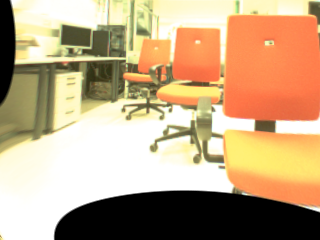
\includegraphics[scale=.3]{chapters/05_experiments/02_depth_map_parameter_tuning/l_rgb.png}}
	\subcaptionbox{}%
	[.4\linewidth]{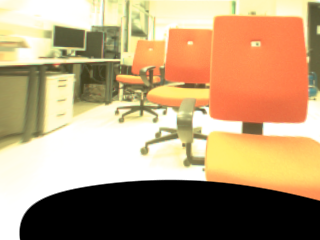
\includegraphics[scale=.3]{chapters/05_experiments/02_depth_map_parameter_tuning/r_rgb.png}}
	\caption{Heicub's perspective of the scene for the setup in figure \ref{fig::52_wls_setup}. (a) shows the left camera's view, while (b) shows the right camera's view.}
	\label{fig::52_wls_rgb}
\end{figure}

\begin{figure}[h]
	\centering
	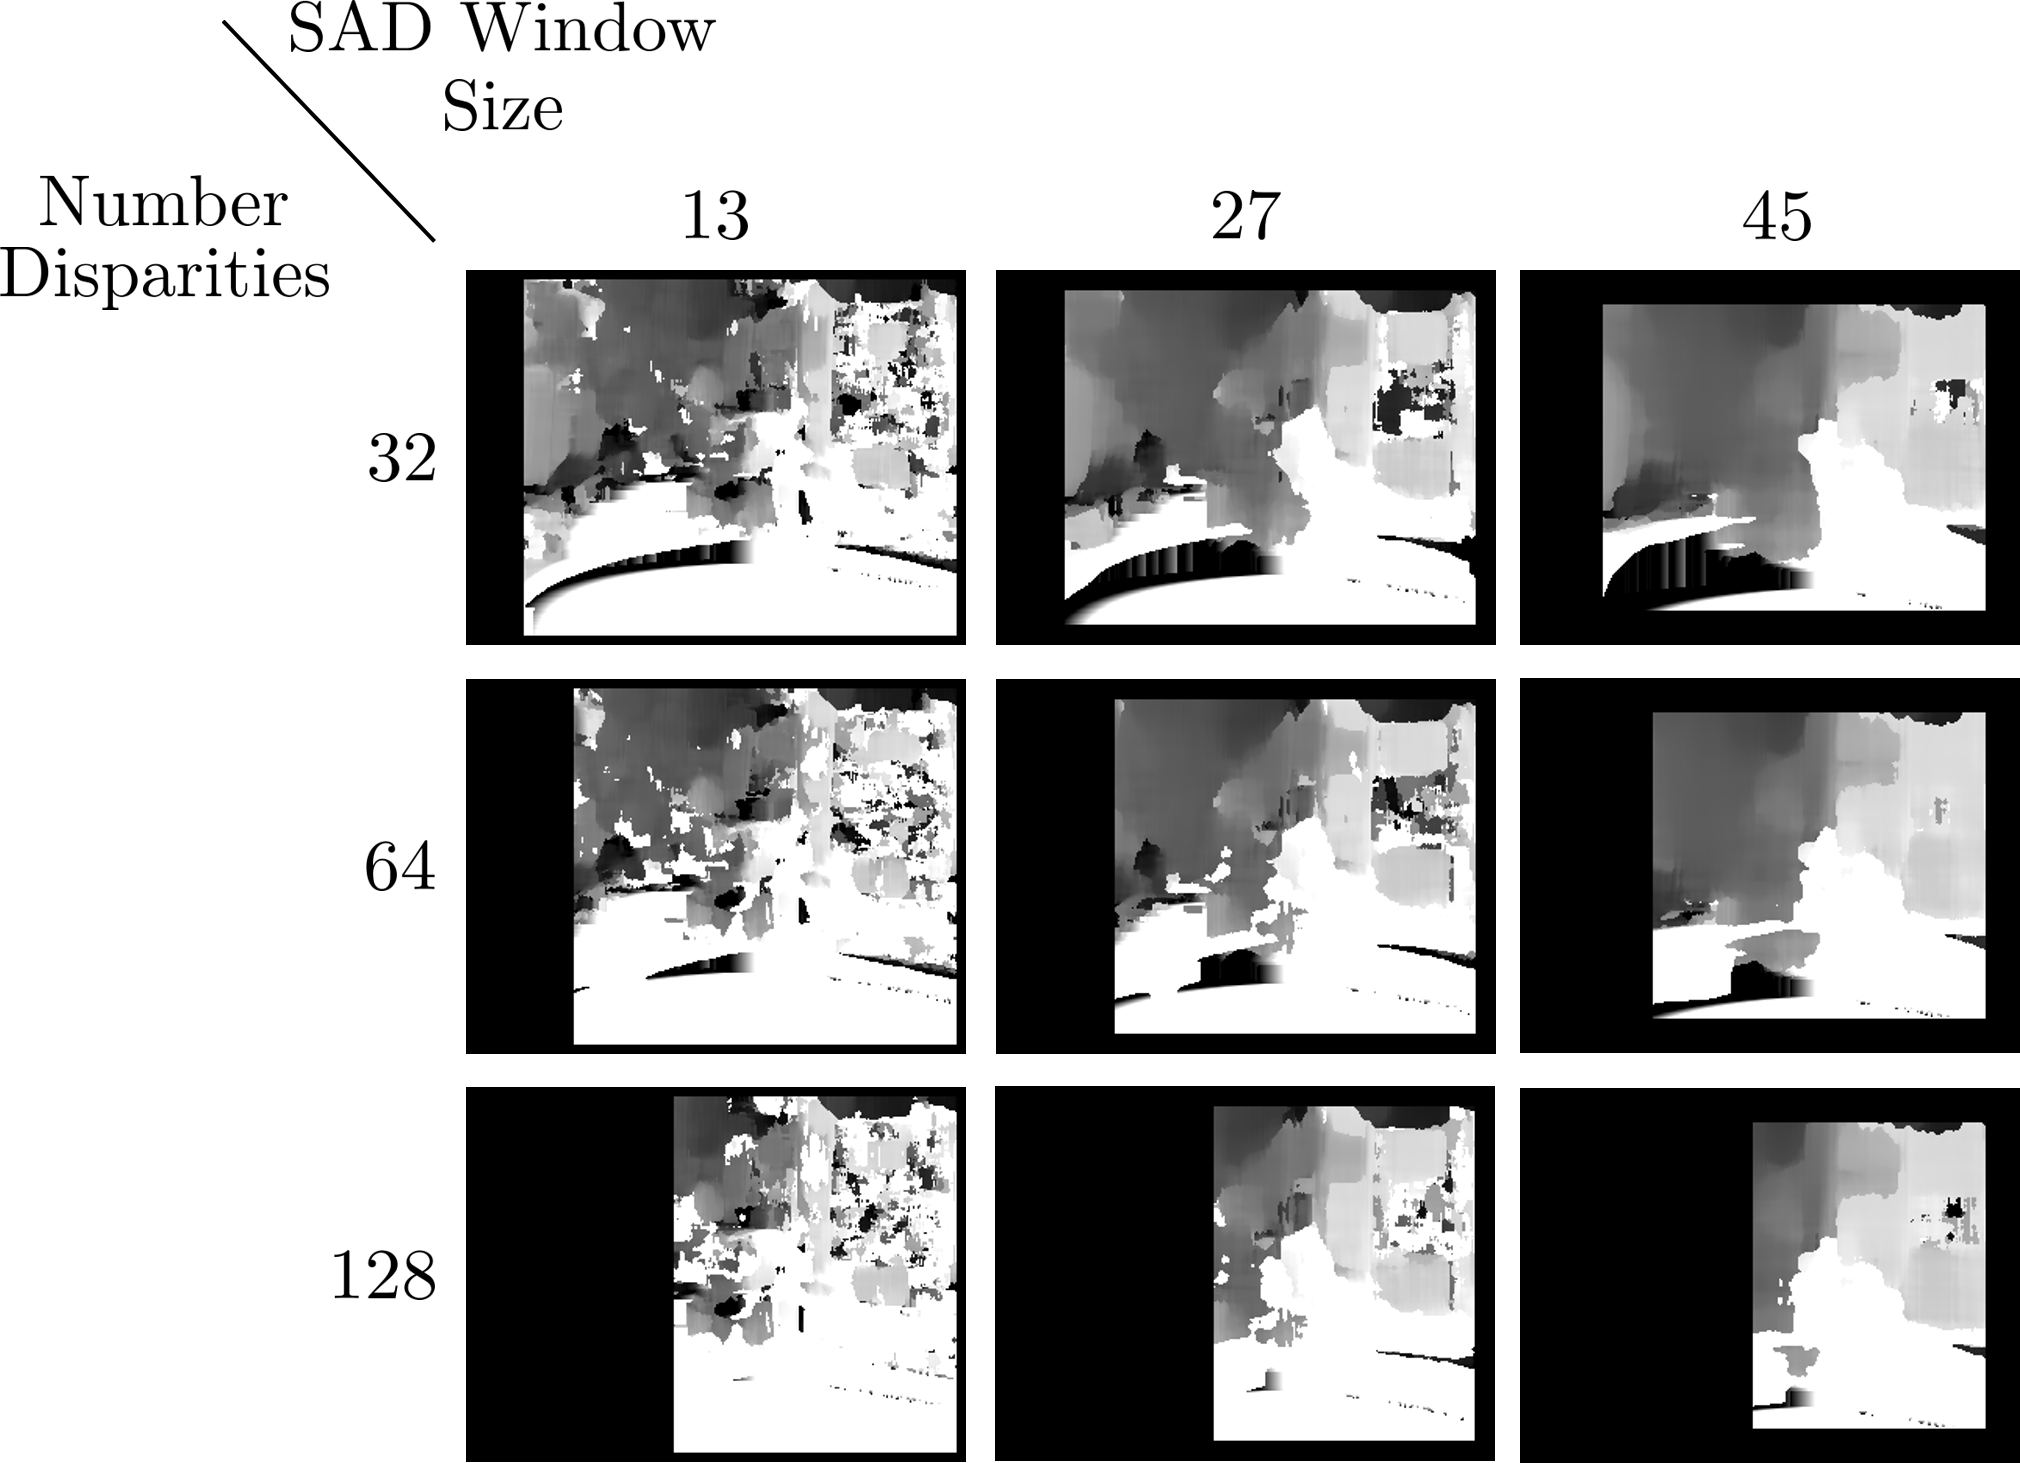
\includegraphics[scale=.25]{chapters/05_experiments/02_depth_map_parameter_tuning/disp_sad.png}
	\caption{Left disparity map for changing SAD window sizes and number of disparities. Please refer to figure \ref{fig::324_left_disparity_map} and equation \ref{eq::324_sad} for the theory.}
	\label{fig::52_disp_sad}
\end{figure}
\begin{figure}[h]
	\centering
	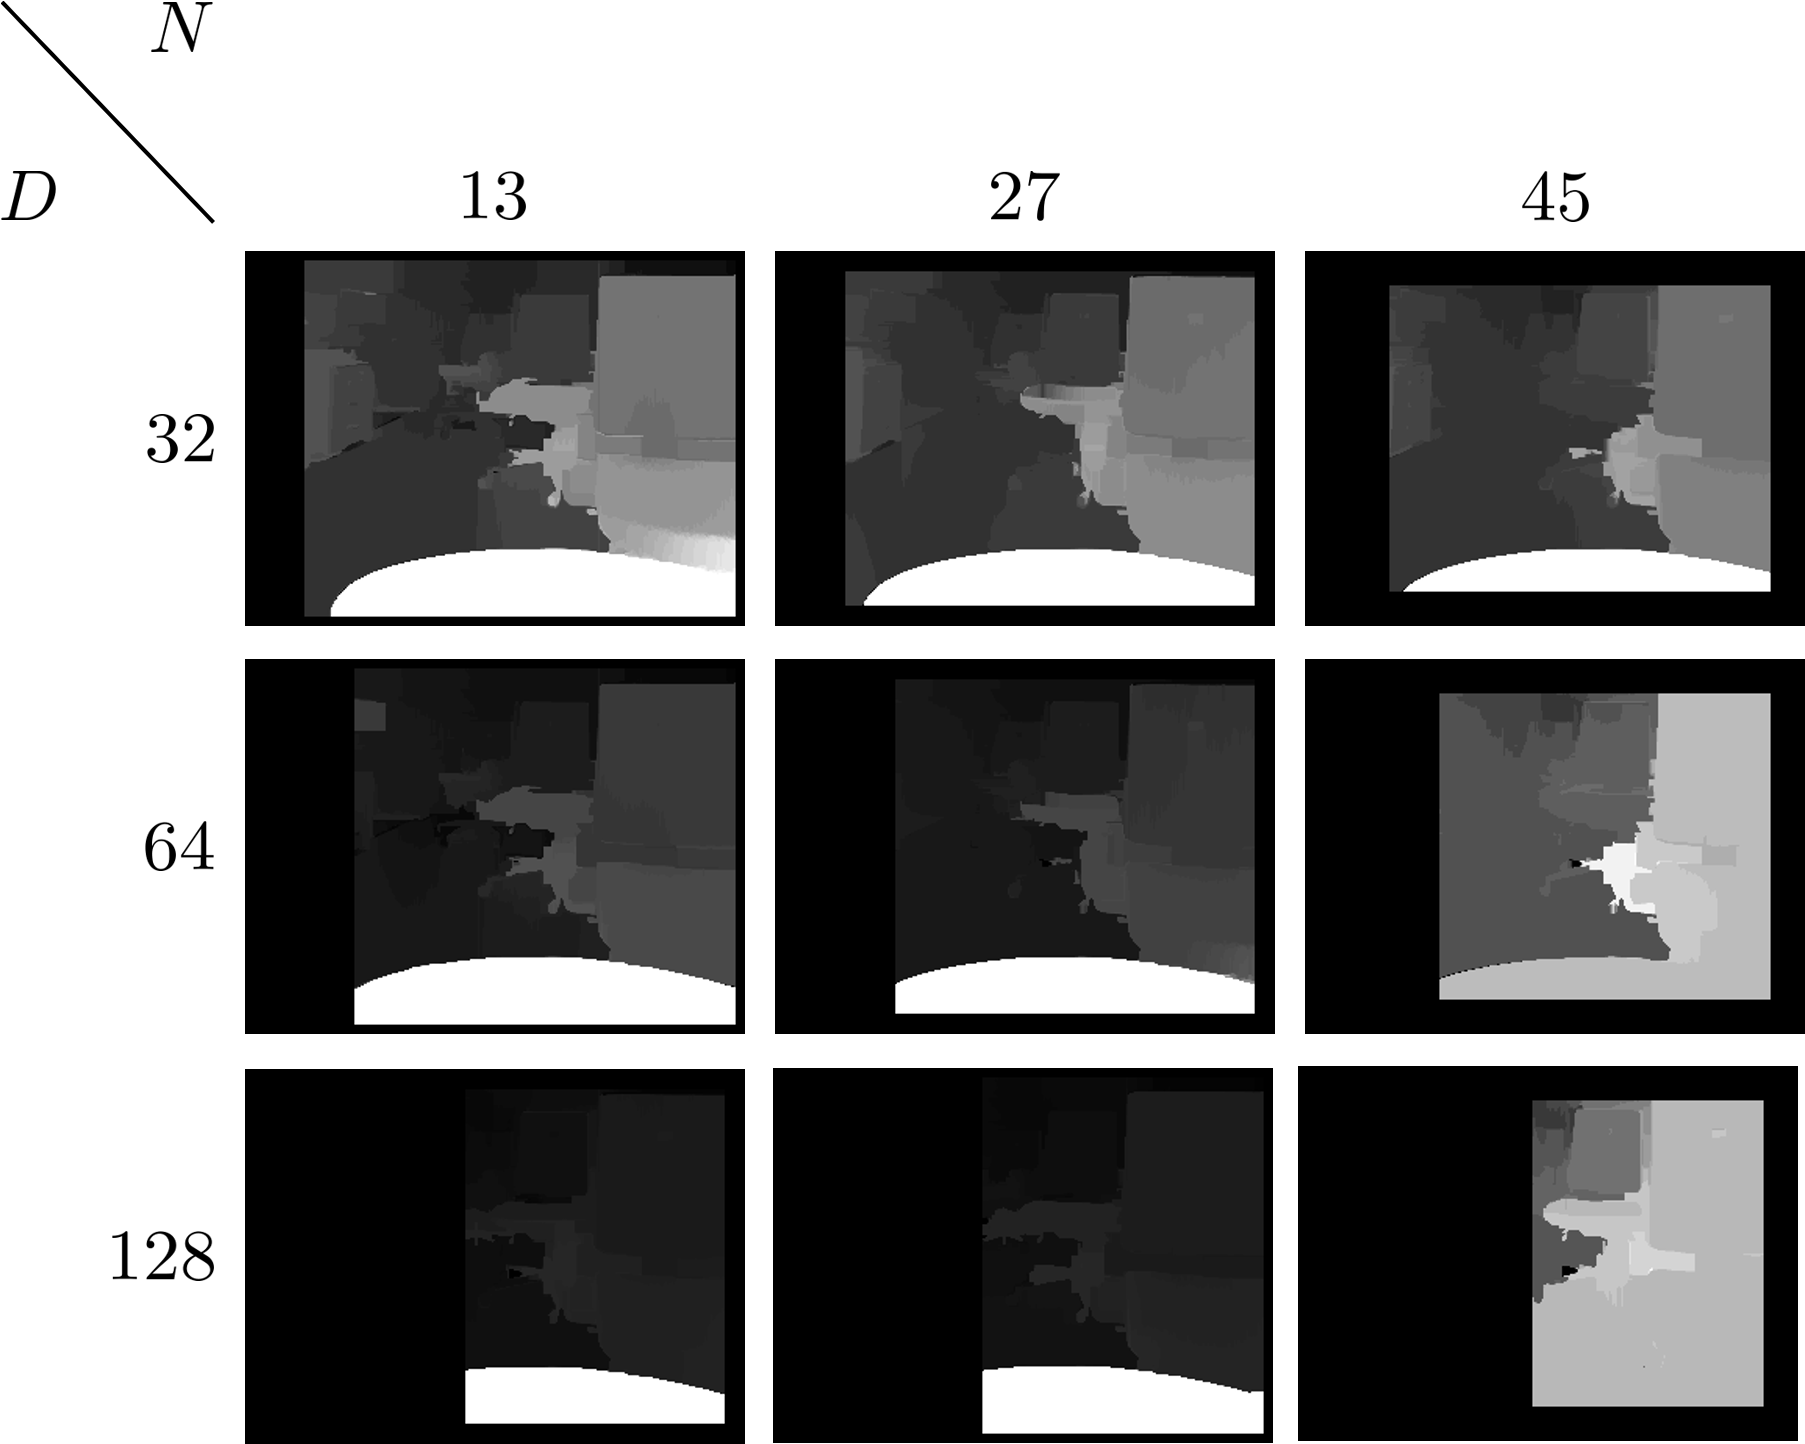
\includegraphics[scale=.25]{chapters/05_experiments/02_depth_map_parameter_tuning/disp_sad_wls.png}
	\caption{Confidence weighted least squares disparity for changing SAD windows sizes and number of disparities. Please refer to figure \ref{fig::324_weighted_least_squares_disparity} and equation \ref{eq::324_wls_final} for the theory.}
	\label{fig::52_disp_sad_wls}
\end{figure}
\begin{figure}[h]
	\centering
	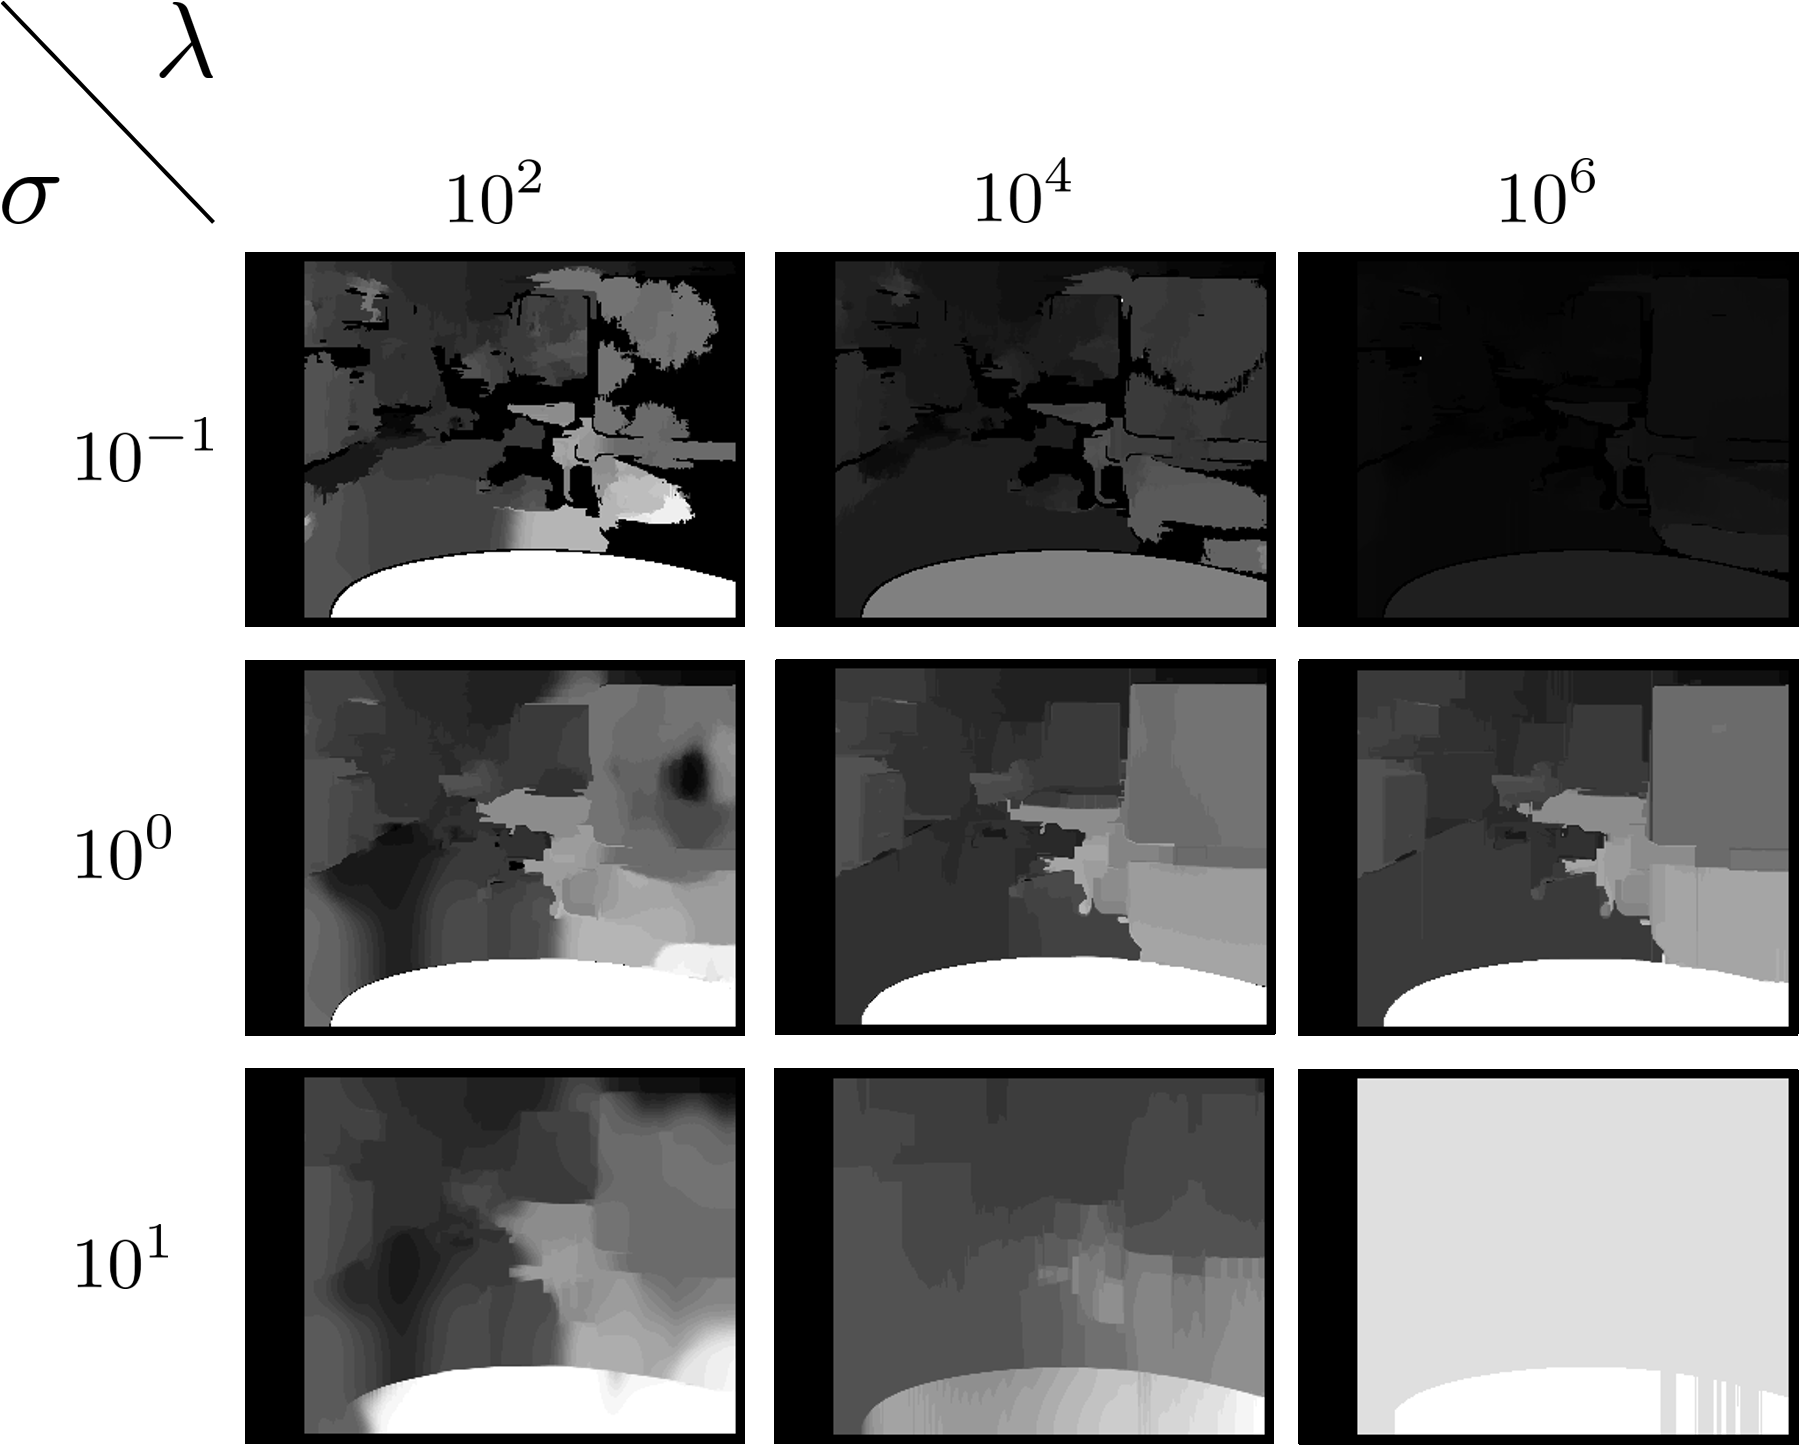
\includegraphics[scale=.25]{chapters/05_experiments/02_depth_map_parameter_tuning/sigma_lambda.png}
	\caption{$\sigma$\ref{eq::324_weight} $\lambda$\ref{eq::324_energy_function}}
	\label{fig::52_sigma_lambda}
\end{figure}
\begin{figure}[h]
	\centering
	\subcaptionbox{}%
	[.4\linewidth]{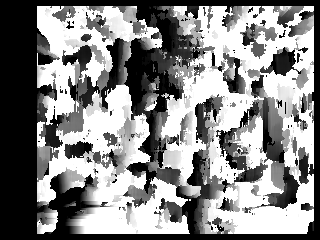
\includegraphics[scale=.3]{chapters/05_experiments/02_depth_map_parameter_tuning/disp_no_calib.png}}
	\subcaptionbox{}%
	[.4\linewidth]{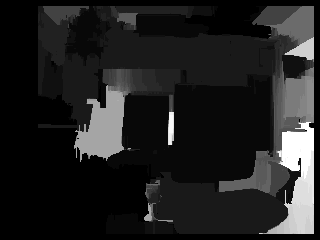
\includegraphics[scale=.3]{chapters/05_experiments/02_depth_map_parameter_tuning/wls_no_calib.png}}
	\caption{Disparity map, and confidence weighted least squares disparity map without rectification.}
	\label{fig::52_no_calib}
\end{figure}
  \section{User Controlled Walking}
\label{sec::53_uc}
\subsection{Performance in Test Environment}
\begin{figure}[h]
	\centering
	\subcaptionbox{Straight Walk - Dynamic Balance}%
	[.4\linewidth]{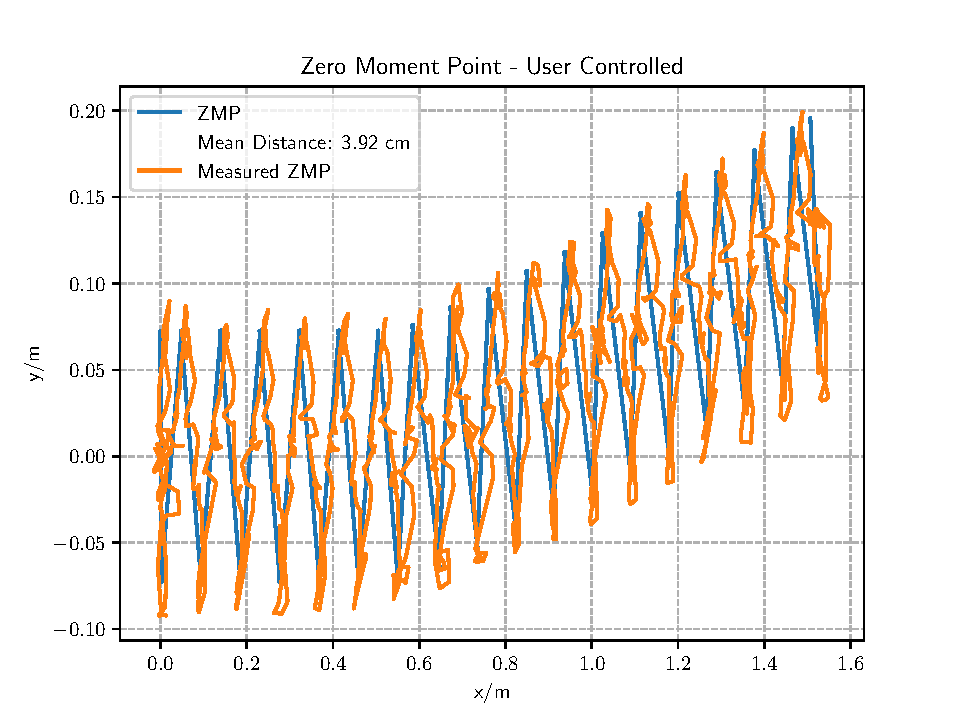
\includegraphics[scale=.35]{chapters/05_experiments/03_user_controlled_walking/straight_walk_01_zmp.pdf}}
	\subcaptionbox{Straight Walk - Behavior}%
	[.4\linewidth]{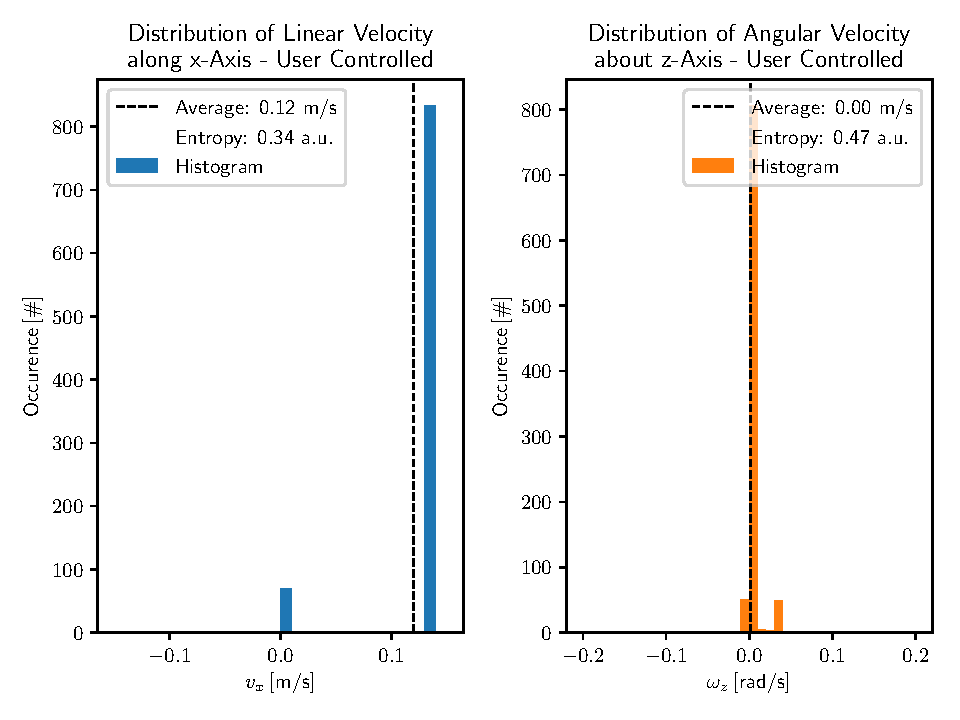
\includegraphics[scale=.35]{chapters/05_experiments/03_user_controlled_walking/straight_walk_01_entropy.pdf}}
	\subcaptionbox{Curved Walk - Dynamic Balance}%
	[.4\linewidth]{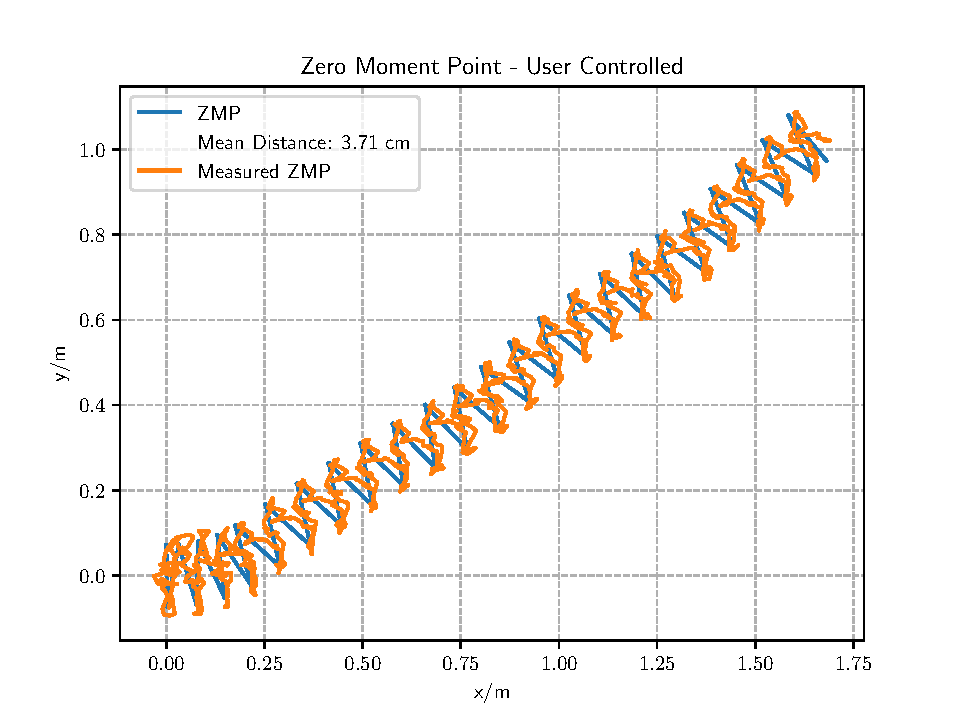
\includegraphics[scale=.35]{chapters/05_experiments/03_user_controlled_walking/curved_walk_01_zmp.pdf}}
	\subcaptionbox{Curved Walk - Behavior}%
	[.4\linewidth]{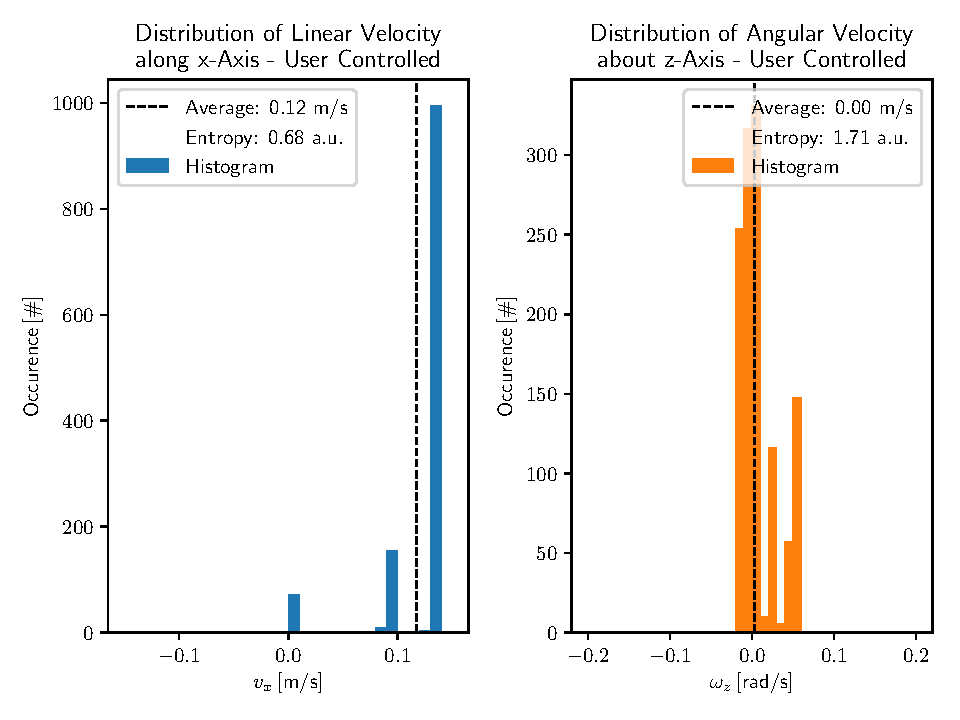
\includegraphics[scale=.35]{chapters/05_experiments/03_user_controlled_walking/curved_walk_01_entropy.pdf}}
	\subcaptionbox{Obstacle Avoidance - Dynamic Balance}%
	[.4\linewidth]{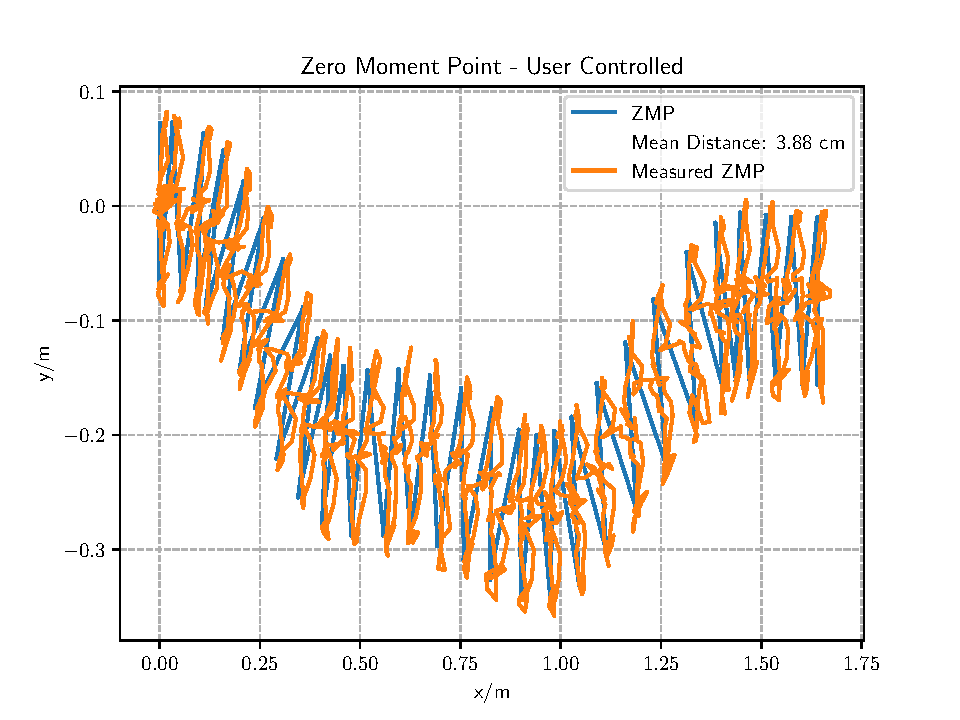
\includegraphics[scale=.35]{chapters/05_experiments/03_user_controlled_walking/obstacle_walk_02_zmp.pdf}}
	\subcaptionbox{Obstacle Avoidance - Behavior}%
	[.4\linewidth]{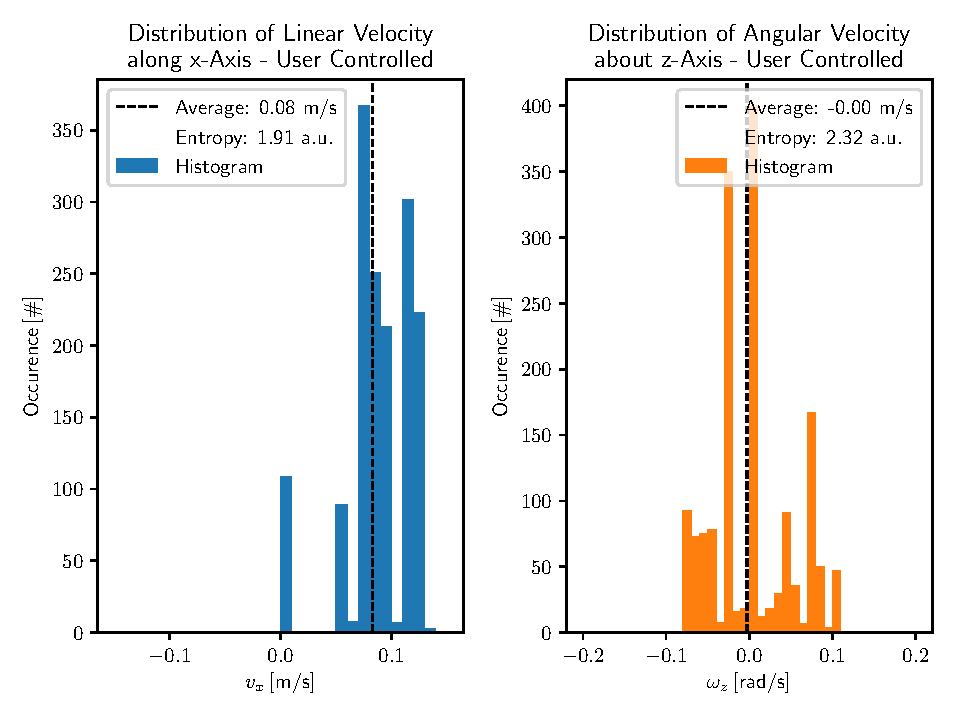
\includegraphics[scale=.35]{chapters/05_experiments/03_user_controlled_walking/obstacle_walk_02_entropy.pdf}}
	\subcaptionbox{Environment Scanning - Dynamic Balance}%
	[.4\linewidth]{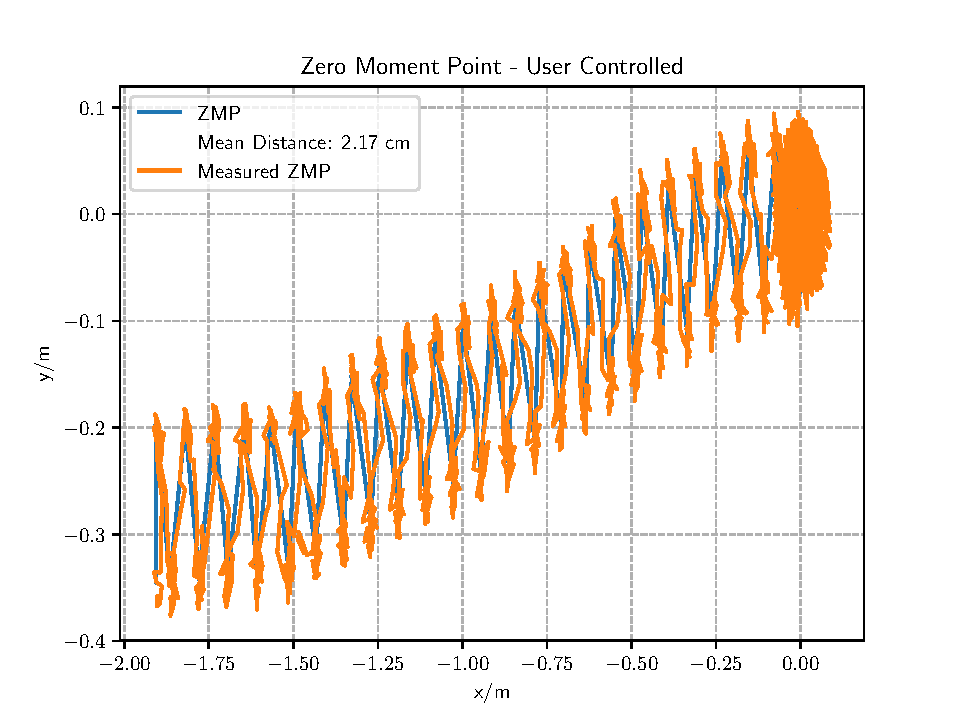
\includegraphics[scale=.35]{chapters/05_experiments/03_user_controlled_walking/out_of_sight_walk_01_zmp.pdf}}
	\subcaptionbox{Environment Scanning - Behavior}%
	[.4\linewidth]{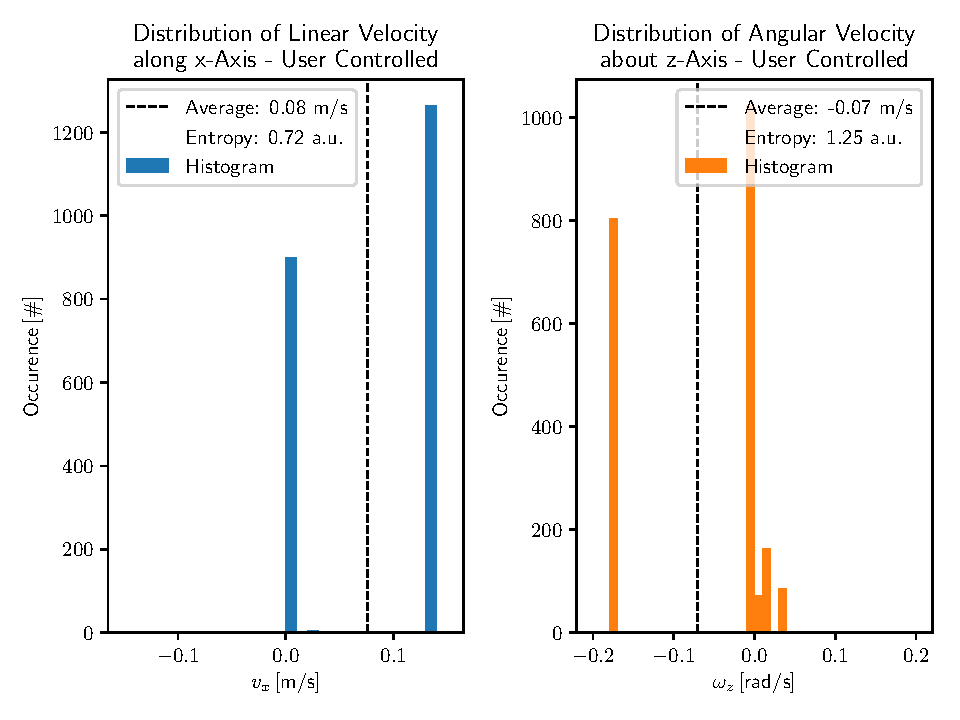
\includegraphics[scale=.35]{chapters/05_experiments/03_user_controlled_walking/out_of_sight_walk_01_entropy.pdf}}
	\caption{}
	\label{fig::52_uc_basic}
\end{figure} 
  \section{Autonomous Walking}
\label{sec::54_aw}
\subsection{Data Acquisition}
\label{sec::541_da}
\begin{figure}[h]
	\centering
	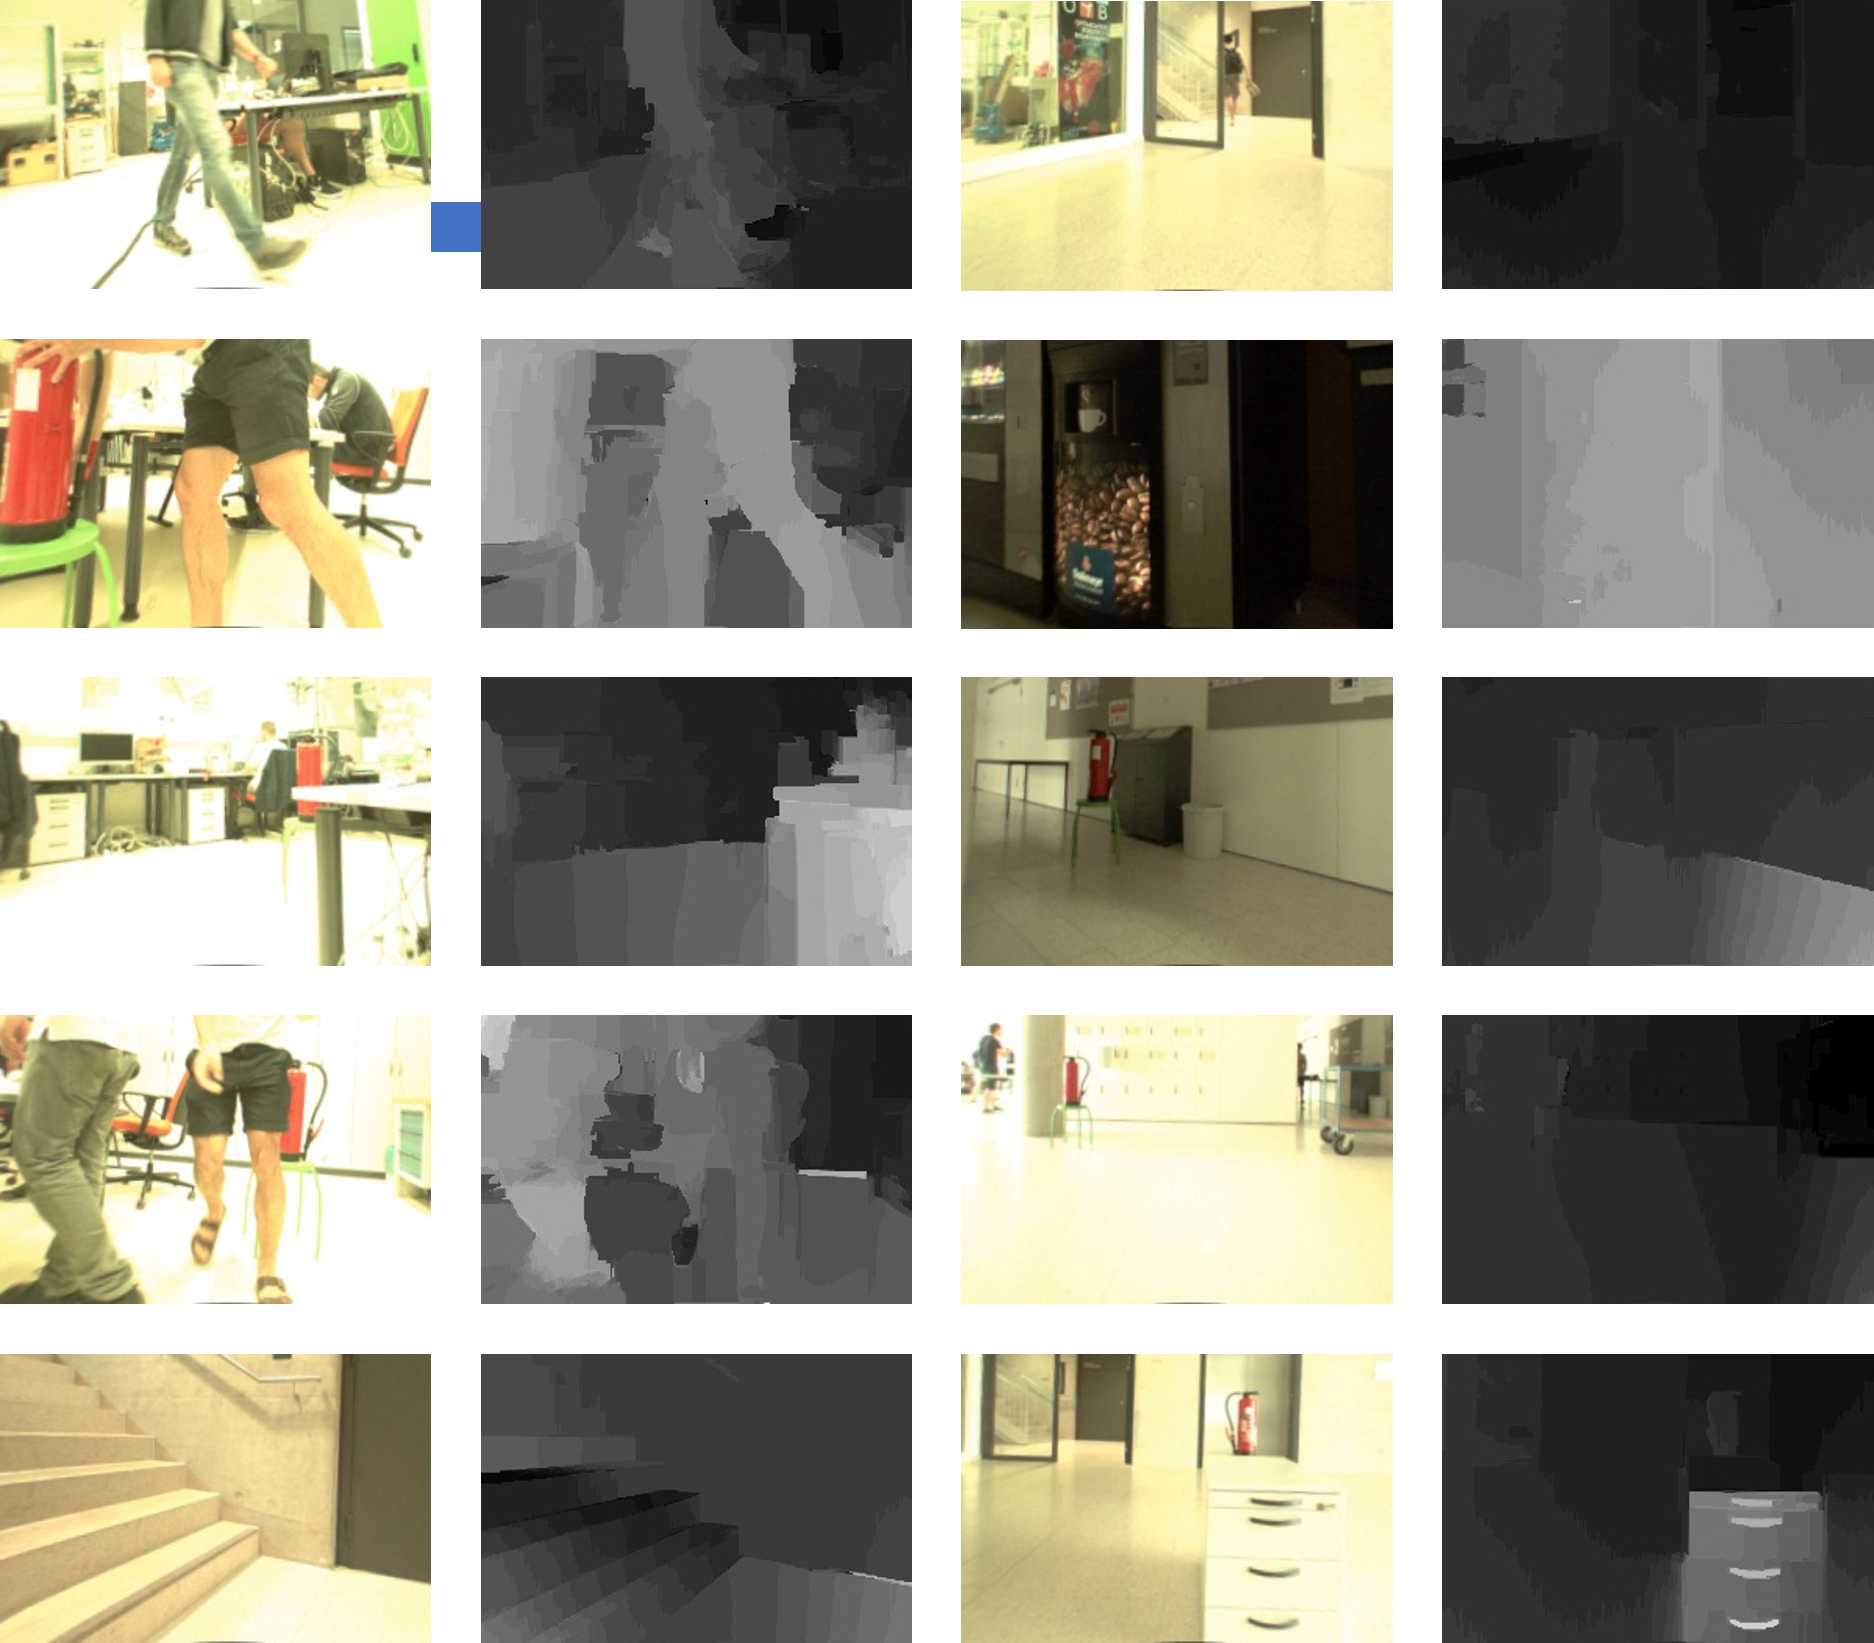
\includegraphics[scale=.4]{chapters/05_experiments/04_autonomous_walking/dataset_diversity.png}
	\caption{}
	\label{fig::542_dataset}
\end{figure}
\subsection{Network Architecture and Training}
\begin{figure}[h]
	\centering
	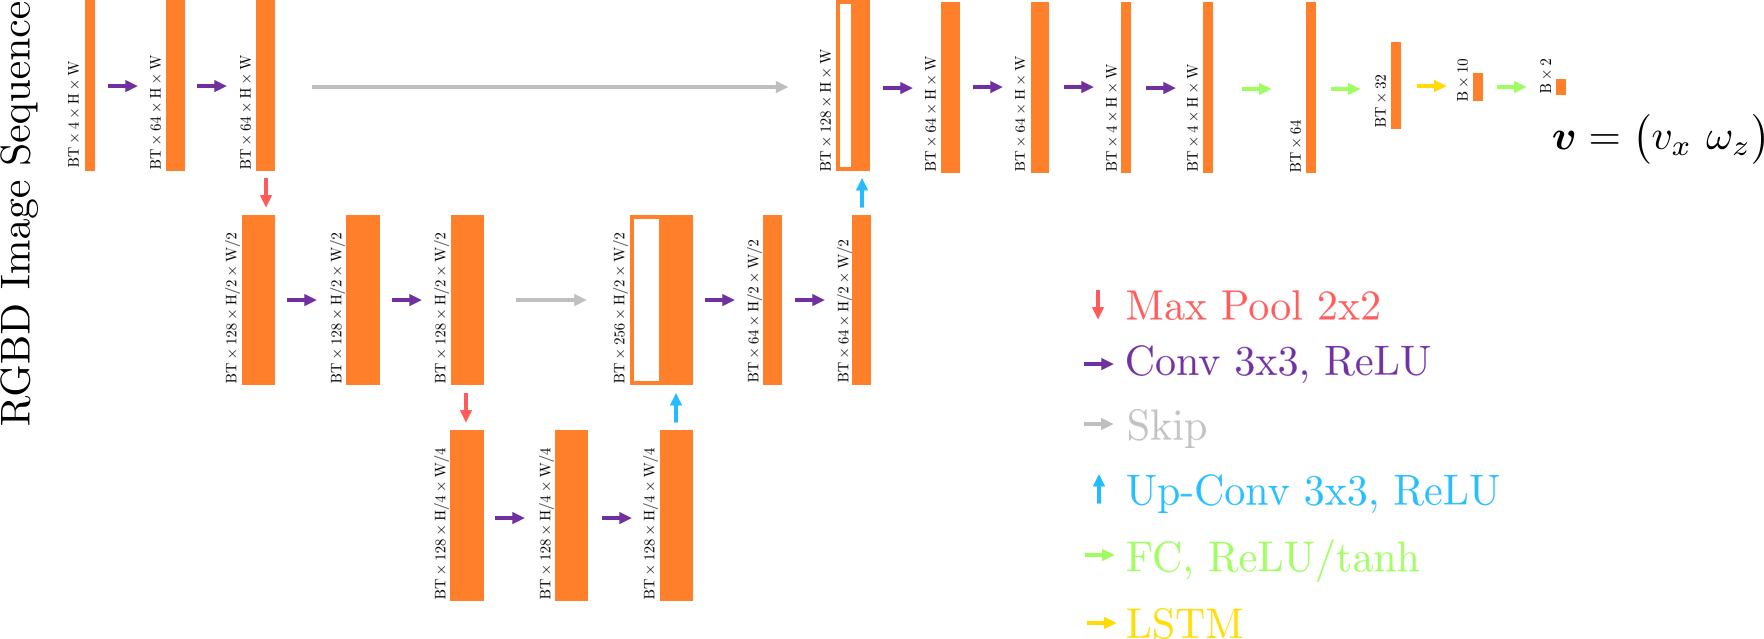
\includegraphics[scale=.5]{chapters/05_experiments/04_autonomous_walking/unet.png}
	\caption{}
	\label{fig::542_unet}
\end{figure}
\begin{figure}[h]
	\centering
	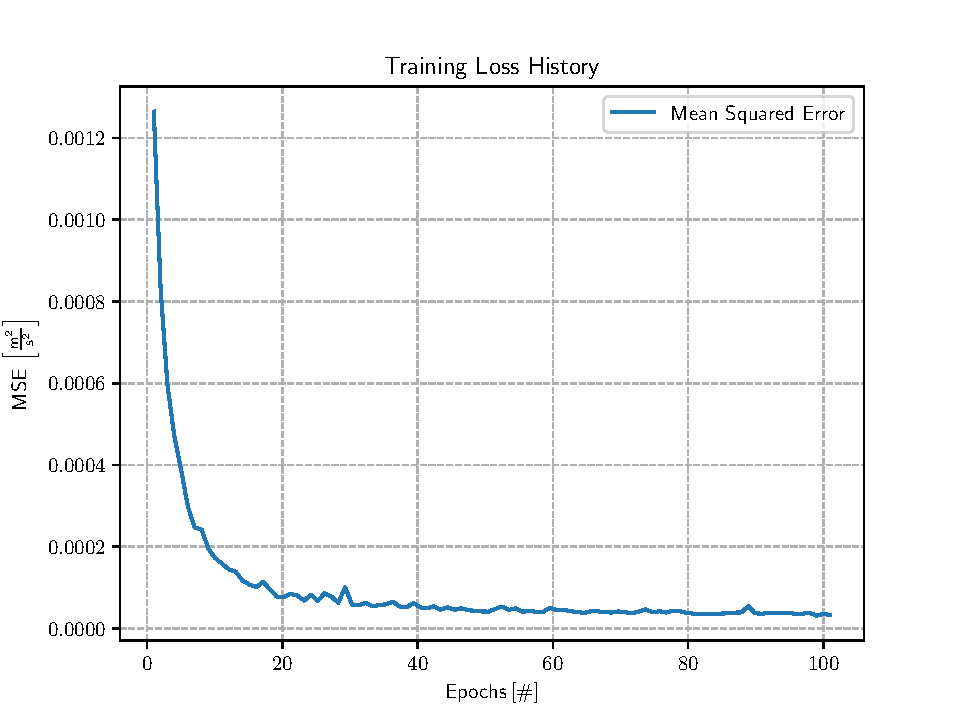
\includegraphics[scale=.6]{chapters/05_experiments/04_autonomous_walking/05_07_19_loss_history.pdf}
	\caption{}
	\label{fig::542_loss}
\end{figure}
\begin{figure}[h]
	\centering
	\subcaptionbox{}%
	[.4\linewidth]{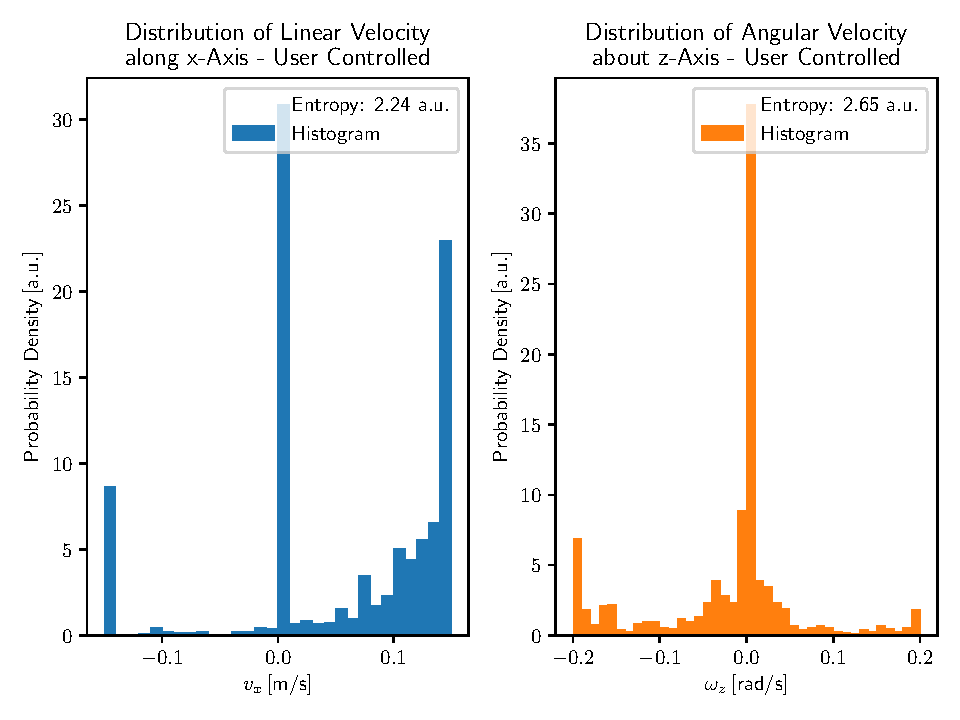
\includegraphics[scale=.35]{chapters/05_experiments/04_autonomous_walking/user_entropy.pdf}}
	\subcaptionbox{}%
	[.4\linewidth]{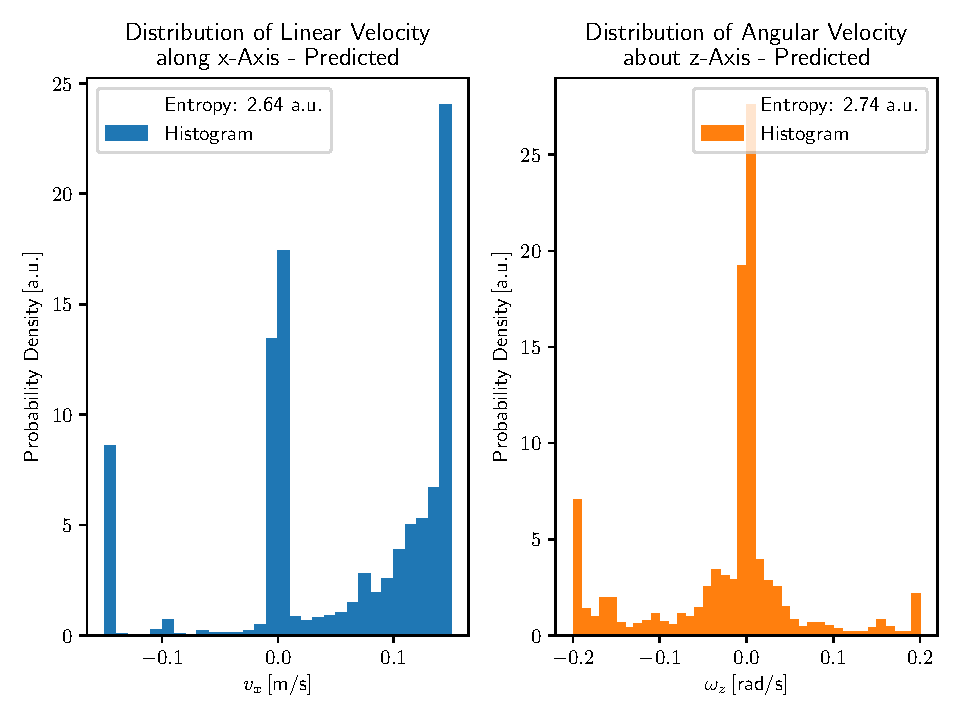
\includegraphics[scale=.35]{chapters/05_experiments/04_autonomous_walking/predicted_entropy_kldivx_0_33_kldivz_0_06_imgs_13441_duration_4_ms.pdf}}
	\caption{KL divergence x 0.33, KL divergence z 0.06, validation split on 13441 imgs, average duration 4 ms}
	\label{fig::542_training_dist}
\end{figure}
% compute kl divergence for whole set -> argue that this holds true for all 
\subsection{Performance in Test Environment}
\begin{figure}[h]
	\centering
	\subcaptionbox{Straight Walk}%
	[.4\linewidth]{\animategraphics[height=1.2in,loop,autoplay]{20}{chapters/05_experiments/04_autonomous_walking/straight_walk_01/frame-}{001}{033}}
	\subcaptionbox{Curved Walk}%
	[.4\linewidth]{\animategraphics[height=1.2in,loop,autoplay]{20}{chapters/05_experiments/04_autonomous_walking/curved_walk_02/frame-}{001}{039}}
	\subcaptionbox{Obstacle Avoidance}%
	[.4\linewidth]{\animategraphics[height=1.2in,loop,autoplay]{20}{chapters/05_experiments/04_autonomous_walking/obstacle_walk_02/frame-}{001}{017}}
	\subcaptionbox{Environment Scanning}%
	[.4\linewidth]{\animategraphics[height=1.2in,loop,autoplay]{20}{chapters/05_experiments/04_autonomous_walking/out_of_sight_walk_01/frame-}{001}{075}}
	\caption{}
	\label{fig::53_aw_gif_basic}
\end{figure} 
\begin{figure}[h]
	\centering
	\subcaptionbox{Straight Walk - Dynamic Balance}%
	[.4\linewidth]{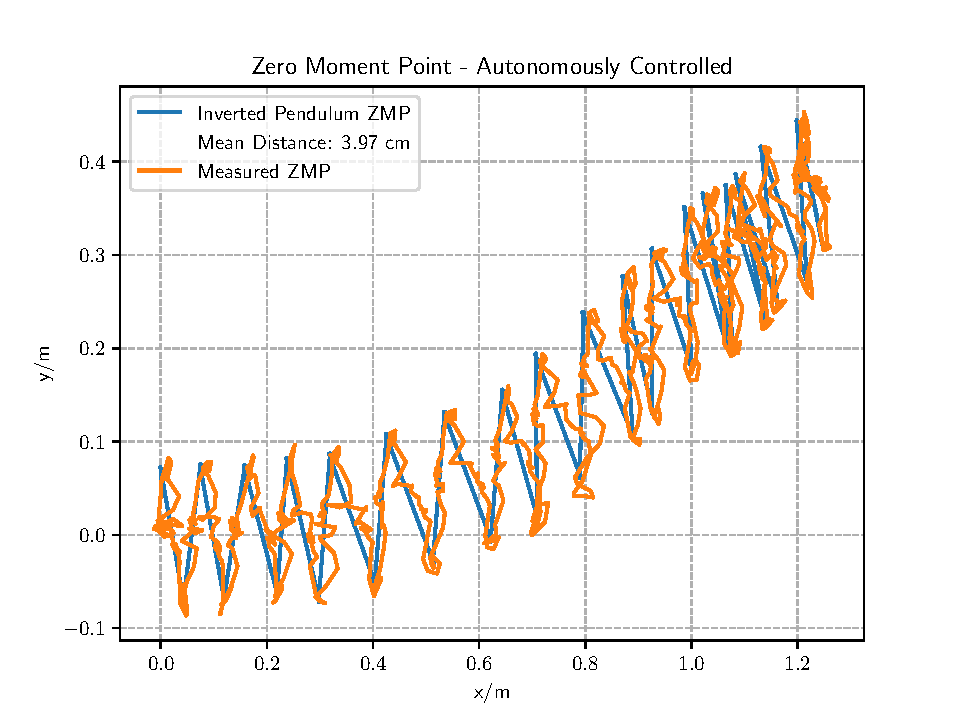
\includegraphics[scale=.35]{chapters/05_experiments/04_autonomous_walking/straight_walk_01_zmp.pdf}}
	\subcaptionbox{Straight Walk - Behavior}%
	[.4\linewidth]{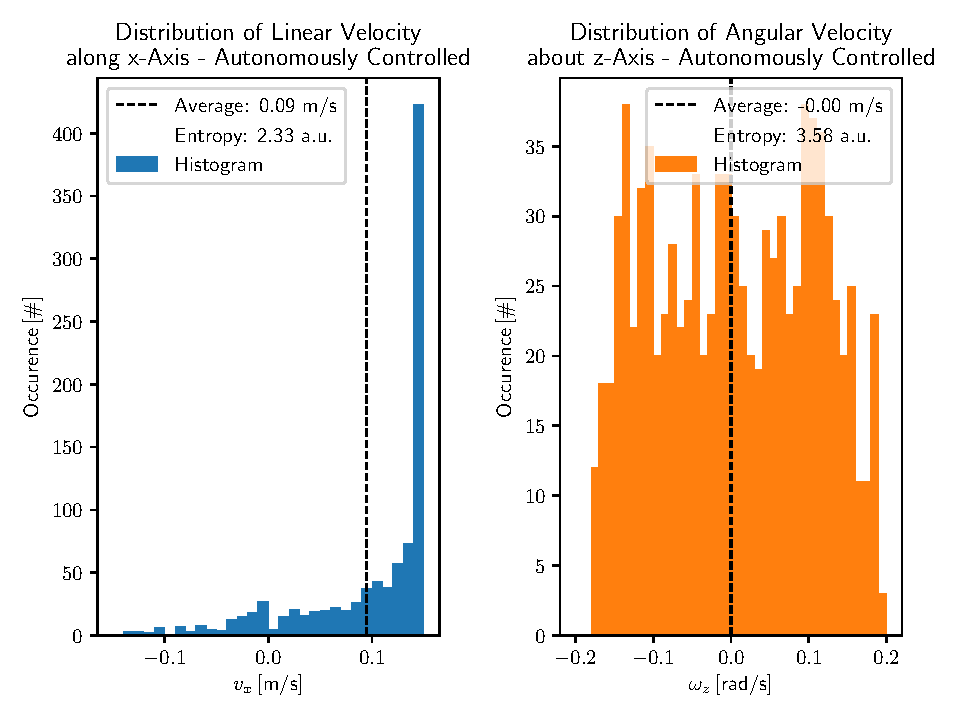
\includegraphics[scale=.35]{chapters/05_experiments/04_autonomous_walking/straight_walk_01_entropy.pdf}}
	\subcaptionbox{Curved Walk - Dynamic Balance}%
	[.4\linewidth]{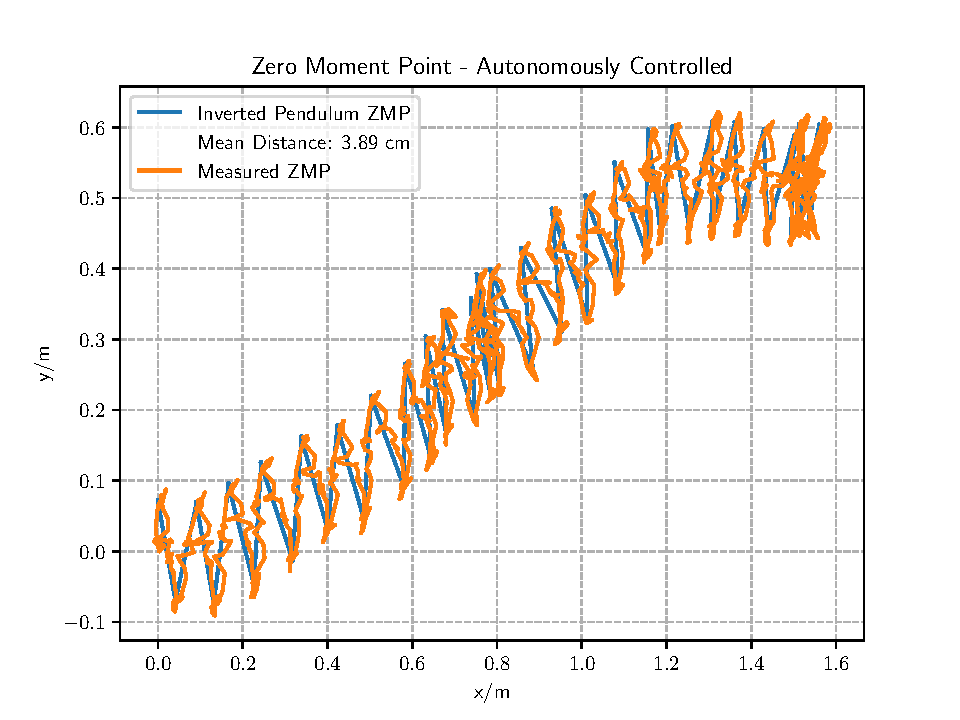
\includegraphics[scale=.35]{chapters/05_experiments/04_autonomous_walking/curved_walk_01_zmp.pdf}}
	\subcaptionbox{Curved Walk - Behavior}%
	[.4\linewidth]{\includegraphics[scale=.35]{chapters/05_experiments/04_autonomous_walking/curved_walk_01_entropy.pdf}}
	\subcaptionbox{Obstacle Avoidance - Dynamic Balance}%
	[.4\linewidth]{\includegraphics[scale=.35]{chapters/05_experiments/04_autonomous_walking/obstacle_walk_02_zmp.pdf}}
	\subcaptionbox{Obstacle Avoidance - Behavior}%
	[.4\linewidth]{\includegraphics[scale=.35]{chapters/05_experiments/04_autonomous_walking/obstacle_walk_02_entropy.pdf}}
	\subcaptionbox{Environment Scanning - Dynamic Balance}%
	[.4\linewidth]{\includegraphics[scale=.35]{chapters/05_experiments/04_autonomous_walking/out_of_sight_walk_01_zmp.pdf}}
	\subcaptionbox{Environment Scanning - Behavior}%
	[.4\linewidth]{\includegraphics[scale=.35]{chapters/05_experiments/04_autonomous_walking/out_of_sight_walk_01_entropy.pdf}}
	\caption{}
	\label{fig::53_aw_basic}
\end{figure} 
\begin{figure}[h]
	\centering
	\subcaptionbox{Dynamic Environment}%
	[.4\linewidth]{\animategraphics[height=1.2in,loop,autoplay]{20}{chapters/05_experiments/04_autonomous_walking/dynamic_walk_01/frame-}{001}{031}}
	\subcaptionbox{Semantic Understanding}%
	[.4\linewidth]{\animategraphics[height=1.2in,loop,autoplay]{20}{chapters/05_experiments/04_autonomous_walking/semantic_walk_01/frame-}{001}{046}}
	\caption{}
\label{fig::53_aw_gif_additional}
\end{figure} 
\begin{figure}[h]
	\centering
	\subcaptionbox{Dynamic Environment - Dynamic Balance}%
	[.4\linewidth]{\includegraphics[scale=.35]{chapters/05_experiments/04_autonomous_walking/dynamic_walk_01_zmp.pdf}}
	\subcaptionbox{Dynamic Environment - Behavior}%
	[.4\linewidth]{\includegraphics[scale=.35]{chapters/05_experiments/04_autonomous_walking/dynamic_walk_01_entropy.pdf}}
	\subcaptionbox{Semantic Understanding - Dynamic Balance}%
	[.4\linewidth]{\includegraphics[scale=.35]{chapters/05_experiments/04_autonomous_walking/semantic_walk_01_zmp.pdf}}
	\subcaptionbox{Semantic Understanding - Behavior}%
	[.4\linewidth]{\includegraphics[scale=.35]{chapters/05_experiments/04_autonomous_walking/semantic_walk_01_entropy.pdf}}
	\caption{}
	\label{fig::53_aw_additional}
\end{figure}
\begin{figure}[h]
	\centering
	\includegraphics[scale=.6]{chapters/05_experiments/04_autonomous_walking/entropy_against_balance.pdf}
	\caption{meanaw 3.67, meanuc 3.41, stdaw 0.56, stduc 0.69}
	\label{fig::542_entropy_balance}
\end{figure}
\subsection{Proximal Policy Optimization}

  %\section{Reinforcement Learning}
\label{sec::55_rl}

  \chapter{Conclusion}
  \section{Contributions}
\label{sec::61_co}
% implemented fully functional nmpc
% app
% behavioral cloning
% proximal policy optimization -> rbdl
  \section{Future Work}
\label{sec::61_fw}
% behavioral cloning -> general purpose navigation
% ppo -> learn solutions


  \part{Appendix}
  \begin{appendix}
  	\chapter{Software Installation}
\label{sec::A_si}
Since all of the software is freely available on GitHub, you can always find a build section within the provided readme file there. The links to the respective GitHub folders are provided within each following section. For the case of an error that may occur during the build procedure, do no hesitate to open up an issue there. I will then help you to get the software running on your device.
\section{Build the Pattern Generator}
\label{sec::A1_pg}
\section{Build the Android Joystick App}
\label{sec::A2_aa}
\section{Build Proximal Policy Optimization}
\section{Build Simulation Models}
\label{sec::A4_sm}
\section{Build Third Party Software}
\label{sec::A5_tp}
  	\chapter{Startup and Shutdown Procedures}
\label{sec::B_su}
In this chapter, we will briefly document how to run the software that was developed within this thesis. In section \ref{sec::B1_rr}, we will introduce how the Heicub robot is supposed to be started, while in the subsequent section \ref{sec::B2_ss}, we will explain how to run the robot within the simulation environment Gazebo. Furthermore, once the robot has been started, either in real or in simulation, it is possible to use the provided pattern generator for control in realtime with the terminal interface or the Android joysitck app. Both possibilities will be explained in section \ref{sec::B3_sp}. Finally, a short demonstration for the behavioral augmentation is given in section \ref{sec::B4_ba}.
\section{Real Robot Startup}
\label{sec::B1_rr}
\begin{enumerate}
	\item Turn on the icubsrv (figure \ref{fig::B1_icubsrv}), username is \inlinecode{bash}{icub}, password is \inlinecode{bash}{icub}.
	\begin{figure}[h]
		\centering
		\includegraphics[scale=.04]{chapters/07_appendix/img/icubsrv.jpg}
		\caption{The icubsrv is the Dell laptop. Below it the switch.}
		\label{fig::B1_icubsrv}
	\end{figure}
	\item Turn on the power suppliers (figure \ref{fig::B1_ps}), and keep the red button pressed (figure \ref{fig::B1_red} (a)). The suppliers should initially provide 13V and 0V, if not, do no proceed.
	\begin{figure}[h]
		\centering
		\subcaptionbox{Turn on these buttons.}%
		[.4\linewidth]{\includegraphics[scale=.04]{chapters/07_appendix/img/power_supply.jpg}}
		\subcaptionbox{Expected initial voltage.}%
		[.4\linewidth]{\includegraphics[scale=.04]{chapters/07_appendix/img/power_supply_13.jpg}}
		\caption{Power suppliers.}
		\label{fig::B1_ps}
	\end{figure}
	\item Turn on the pc104 (figure \ref{fig::B1_cpu_motor} (a)). At this step you may want to wait up to 5 minutes, to give the board computer enough time to start.
	\begin{figure}[h]
		\centering
		\subcaptionbox{Turn on the CPU of pc104.}%
		[.4\linewidth]{\includegraphics[scale=.04]{chapters/07_appendix/img/switch_cpu.jpg}}
		\subcaptionbox{Turn on the motors of Heicub.}%
		[.4\linewidth]{\includegraphics[scale=.04]{chapters/07_appendix/img/switch_cpu_motor.jpg}}
		\caption{Heicub's switches.}
		\label{fig::B1_cpu_motor}
	\end{figure}
	\item On the icubsrv, connect via ssh to pc104. Therefore, click on the highlighted symbol within figure \ref{fig::B1_pc104} (a). If it fails to connect, turn off the CPU, and go back to the previous step.
	\begin{figure}[h]
		\centering
		\subcaptionbox{Run ssh to connect to pc104.}%
		[.4\linewidth]{\includegraphics[scale=.326]{chapters/07_appendix/img/task_bar.png}}
		\subcaptionbox{Terminal to pc104.}%
		[.4\linewidth]{\includegraphics[scale=.22]{chapters/07_appendix/img/terminal_pc104.png}}
		\caption{Connect to pc104. TODO highlight symbol}
		\label{fig::B1_pc104}
	\end{figure}
	\item Run the cluster manager from a new terminal on the icubsrv, therefore do \newline \inlinecode{}{cd /usr/local/src/robot/icub-main/build-pc104/bin}
	\newline \inlinecode{}{python icub-cluster.py}
	\item Within the cluster manager, run the yarp name server, and then yarp on all other devices (figure \ref{fig::B1_cluster} (a), then (b)).
	\begin{figure}[h]
		\centering
		\subcaptionbox{Run the yarp nameserver.}%
		[.4\linewidth]{\includegraphics[scale=.3]{chapters/07_appendix/img/ran_yarp.png}}
		\subcaptionbox{Run yarp on other devices.}%
		[.4\linewidth]{\includegraphics[scale=.3]{chapters/07_appendix/img/ran_yarp_others.png}}
		\caption{Run yarp. TODO highlight run}
		\label{fig::B1_cluster}
	\end{figure}
	\item We can now turn on the motors and the cameras, as well as to connect our own laptop, which is explained in the following sections.
\end{enumerate}
\subsection{Start the Motors}
\label{sec::B11_sm}
If the real robot is up and running (section \ref{sec::B1_rr}), you can now start Heicub's motors. Therefore proceed as described below.
\begin{enumerate}
	\item Turn on the motors (figure \ref{fig::B1_cpu_motor} (b)). The power suppliers should now show 13V and 40V. Wait until the blue lights at Heicub stopped blinking (figure \ref{fig::B1_blue}).
	\begin{figure}[h]
		\centering
		\includegraphics[scale=.04]{chapters/07_appendix/img/icub_motor_lights.jpg}
		\caption{Blue motor lights.}
		\label{fig::B1_blue}
	\end{figure}	
	\item Release the safety button (figure \ref{fig::B1_red} (b)).
	\begin{figure}[h]
		\centering
		\subcaptionbox{Pressed safety button.}%
		[.4\linewidth]{\includegraphics[scale=.04]{chapters/07_appendix/img/safety_pushed.jpg}}
		\subcaptionbox{Released safety button.}%
		[.4\linewidth]{\includegraphics[scale=.04]{chapters/07_appendix/img/safety.jpg}}
		\caption{Safety button.}
		\label{fig::B1_red}
	\end{figure}
	\item Within your terminal to pc104 (figure \ref{fig::B1_pc104} (b)) run the command \newline \inlinecode{}{yarprobotinterface} \newline This will run all the motor drivers and connect them to the yarp network.
	\item If no errors occured, we can now run the yarpmotorgui to play around with the motors. This step is not necessary. To run the yarpmotorgui, open a new terminal on the icubsrv, and run the command \newline \inlinecode{}{yarpmotorgui} (figure \ref{fig::B11_gui} (a)) \newline Then, press \inlinecode{}{OK}. The motors can now be manipulated from within the GUI (figure \ref{fig::B11_gui} (b)), e.g. by clicking on the house, which will bring all motors to the home position.
	\begin{figure}[h]
		\centering
		\subcaptionbox{Run the yarpmotorgui.}%
		[.4\linewidth]{\includegraphics[scale=.22]{chapters/07_appendix/img/yarpmotorgui_ok.png}}
		\subcaptionbox{The yarpmotorgui.}%
		[.4\linewidth]{\includegraphics[scale=.22]{chapters/07_appendix/img/yarpmotorgui_api.png}}
		\caption{Accessing the motors.}
		\label{fig::B11_gui}
	\end{figure}
	\item The motors may need to be calibrated when the robot runs for a long time. Therefore, lift up the robot, and bring it to the home position via the yarpmotorgui. Then, start a new terminal on pc104 and run the command \newline \inlinecode{}{yarp rpc /wholeBodyDynamics/rpc} \newline In the interface that will open up, type \newline \inlinecode{}{calib all 300}. 
\end{enumerate}
\subsection{Start the Cameras}
If the real robot is up and running (section \ref{sec::B1_rr}), you can now start Heicub's cameras. Therefore proceed as described below.
\begin{enumerate}
	\item Within a new terminal to pc104 (figure \ref{fig::B1_pc104} (a)), do \newline \inlinecode{}{cd ./local/share/yarp/robots/iCubHeidelberg01/camera}\newline Then, start the camera via \newline \inlinecode{}{yarpdev --from dragonfly2_config_left.ini}\newline This will run the left camera and connect it to the yarp network. Repeat the above steps for the right camera, but replace left by right within the \inlinecode{}{.ini} file.
	\item If no errors occured, we can now run a yarpview to see what Heicub sees. This step is not necessary. To run a yarpview, open a new terminal on the icubsrv, and run the command \newline \inlinecode{}{yarpview} (figure \ref{fig::B12_yarpview} (a)) \newline Then, connect a camera to the yarpview. Therefore, open a new terminal on the icubsrv and run the command \newline \inlinecode{}{yarp connect /icub/cam/left /yarpview/img:i} (figure \ref{fig::B12_yarpview} (b)) \newline You should now see an image.
	\begin{figure}[h]
		\centering
		\subcaptionbox{Run a yarpview.}%
		[.4\linewidth]{\includegraphics[scale=.22]{chapters/07_appendix/img/yarpview.png}}
		\subcaptionbox{Connect a camera to the yarpview.}%
		[.4\linewidth]{\includegraphics[scale=.22]{chapters/07_appendix/img/connect_yarpview.png}}
		\caption{Accessing the cameras.}
		\label{fig::B12_yarpview}
	\end{figure}
\end{enumerate}
\subsection{Connect your own Laptop}
Make sure you installed YARP, as described in section \ref{sec::A5_tp}. You can then connect your own laptop via ethernet to the same network as Heicub. Therefore, proceed as described below.
\begin{enumerate}
	\item  Connect a LAN cable to the switch to which the icubsrv is connected as well (figure \ref{fig::B1_icubsrv}). You will then get assigned an IP address within the same domain as the icubserver, such as \inlinecode{}{10.0.0.x}. Check this by running \inlinecode{}{ifconfig}. The IP address of the icubsrv is \inlinecode{}{10.0.0.1}, while that of the pc104 is \inlinecode{}{10.0.0.2}.
	\item  Check the connection by pinging the icubsrv via \inlinecode{}{ping 10.0.0.1}. If this works, skip this point, otherwise you can create a manual connection.  Therefore, search for \inlinecode{}{Network Connections} among your applications and open it. Then, click \inlinecode{}{Add}. If it is not set already, check the hardware address by running \inlinecode{}{ifconfig}, it should show something similar to \inlinecode{}{HWaddr 9C:EB:E8:B2:AB:27}, choose this as your device. Then go to IPv4 settings and set the IP address to \inlinecode{}{10.0.0.3}, the netmask to \inlinecode{}{24}, and the gateway to \inlinecode{}{10.0.0.255}. Then press save.
	\item If you connected successfully, open a terminal on your device and run \newline \inlinecode{}{yarp detect --write} \newline If it does not find the running yarpserver, manually configure the connection via the following commands from a terminal \newline \inlinecode{}{yarp conf 10.0.0.1 1000} \newline \inlinecode{}{yarp namespace /iCubHeidelberg} \newline \inlinecode{}{yarp detect}
\end{enumerate}
\section{Simulation Startup}
\label{sec::B2_ss}
Make sure you installed Gazebo, YARP, and the Gazebo YARP plugins as described in section \ref{sec::A5_tp}. Also, you need to have the simulation model installed, which is described in section \ref{sec::A4_sm}. When these requirements are satisfied, then proceed as described below.
\begin{enumerate}
	\item Open a terminal and start YARP via \newline \inlinecode{}{yarpserver --write} \newline
	\item Open another terminal and start Gazebo via \newline \inlinecode{}{gazebo -s libgazebo_yarp_clock.so}\newline The clock library will thereby synchronize the YARP clock, and the Gazebo clock.
	\item  In Gazebo, go to the \inlinecode{}{Insert} bar, and insert \inlinecode{}{heicub_without_weights}.
\end{enumerate}
\section{Start the Pattern Generator}
\label{sec::B3_sp}
Make sure you installed the pattern generator library as described in section \ref{sec::A1_pg}. The robot needs to be running, either in real (section \ref{sec::B1_rr}, and section \ref{sec::B11_sm}) or in simulation (section \ref{sec::B2_ss}). By construction, the startup procedure for the simulation and the real robot is the same. You can choose to control the robot via the terminal, or the provided Android app. Both possibilities are described below in section \ref{sec::B31_terminal}, and section \ref{sec::B32_app}, respectively.
\subsection{Control via the Terminal}
\label{sec::B31_terminal}
The terminal user interface comes with the pattern generator, so there is no additional software that needs to be installed. Proceed as described below.
	\begin{enumerate}
		\item Open a new terminal and go to the shell scripts within the pattern generator folder via \newline \inlinecode{}{cd nmpc\_pattern\_generator/sh} \newline On the icubsrv, this folder is located at \inlinecode{}{/home/icub/TODO}. Then, run the keyboard user interface via \newline \inlinecode{}{sh run\_keyboard\_user\_interface.sh}
	\item The shell script will then ask you to run the robot in real or in simulation, write \inlinecode{}{y} or \inlinecode{}{n} and press enter (figure \ref{fig::B31_keyboard} (a)).
	\item The shell script will then ask you for the mode to run in. Write \inlinecode{}{uc} and press enter (figure \ref{fig::B31_keyboard} (a)).
	\item The user interface will should now show up and explain how to control the robot (figure \ref{fig::B31_keyboard} (b)).
	\begin{figure}[h]
		\centering
		\subcaptionbox{Select the mode to run the pattern generator in.}%
		[.4\linewidth]{\includegraphics[scale=.22]{chapters/07_appendix/img/mode.png}}
		\subcaptionbox{Keyboard user interface.}%
		[.4\linewidth]{\includegraphics[scale=.22]{chapters/07_appendix/img/keyboard_interface.png}}
		\caption{Run the keyboard user interface.}
		\label{fig::B31_keyboard}
	\end{figure}
\end{enumerate}
\subsection{Control via the Android Joystick App}
\label{sec::B32_app}
Make sure you installed the Android joystick app as described in section \ref{sec::A2_aa}.
\section{Start the Behavioral Augmentation Demo}
\label{sec::B4_ba}
\section{Real Robot Shutdown}
    \chapter{Lists}
    \listoffigures
    \listoftables
    \bibliographystyle{unsrt}
    \bibliography{chapters/07_appendix/references}
    \setlength{\parindent}{0em}

Erkl\"{a}rung:\par
\vspace{3\baselineskip}
Ich versichere, dass ich diese Arbeit selbstst\"{a}ndig verfasst habe und keine
anderen als die angegebenen Quellen und Hilfsmittel benutzt habe.\par
\vspace{5\baselineskip}
Heidelberg, den (Datum)\hspace{3cm}\dotfill

  \end{appendix}
\end{document}
